%------------------------------------------------------------------------------
% Template file for the submission of papers to IUCr journals in LaTeX2e
% using the iucr document class
% Copyright 1999-2013 International Union of Crystallography
% Version 1.6 (28 March 2013)
%------------------------------------------------------------------------------

\documentclass[preprint]{iucr}              % DO NOT DELETE THIS LINE

     %-------------------------------------------------------------------------
     % Information about journal to which submitted
     %-------------------------------------------------------------------------
     \journalcode{S}              % Indicate the journal to which submitted
                                  %   A - Acta Crystallographica Section A
                                  %   B - Acta Crystallographica Section B
                                  %   C - Acta Crystallographica Section C
                                  %   D - Acta Crystallographica Section D
                                  %   E - Acta Crystallographica Section E
                                  %   F - Acta Crystallographica Section F
                                  %   J - Journal of Applied Crystallography
                                  %   M - IUCrJ
                                  %   S - Journal of Synchrotron Radiation

\begin{document}                  % DO NOT DELETE THIS LINE

     %-------------------------------------------------------------------------
     % The introductory (header) part of the paper
     %-------------------------------------------------------------------------

     % The title of the paper. Use \shorttitle to indicate an abbreviated title
     % for use in running heads (you will need to uncomment it).

\title{Effects of Lattice Strained in Silicon Double Crystal Monochromators}
%\shorttitle{Short Title}

     % Authors' names and addresses. Use \cauthor for the main (contact) author.
     % Use \author for all other authors. Use \aff for authors' affiliations.
     % Use lower-case letters in square brackets to link authors to their
     % affiliations; if there is only one affiliation address, remove the [a].

\cauthor[a]{Johan}{Eckdahl}{johaneckdahl@ucsb.edu}{address if different from \aff}
\author[a]{Peter}{Sondhauss}

\aff[a]{MAX IV Laboratory \country{Sweden}}


     % Use \shortauthor to indicate an abbreviated author list for use in
     % running heads (you will need to uncomment it).

%\shortauthor{Soape, Author and Doe}

     % Use \vita if required to give biographical details (for authors of
     % invited review papers only). Uncomment it.

%\vita{Author's biography}

     % Keywords (required for Journal of Synchrotron Radiation only)
     % Use the \keyword macro for each word or phrase, e.g. 
     % \keyword{X-ray diffraction}\keyword{muscle}

%\keyword{keyword}

     % PDB and NDB reference codes for structures referenced in the article and
     % deposited with the Protein Data Bank and Nucleic Acids Database (Acta
     % Crystallographica Section D). Repeat for each separate structure e.g
     % \PDBref[dethiobiotin synthetase]{1byi} \NDBref[d(G$_4$CGC$_4$)]{ad0002}

%\PDBref[optional name]{refcode}
%\NDBref[optional name]{refcode}

\maketitle                        % DO NOT DELETE THIS LINE

\begin{synopsis}
Supply a synopsis of the paper for inclusion in the Table of Contents.
\end{synopsis}

\begin{abstract}
Silicon double crystal monochromators are standard in modern synchrotron hard X-ray beamlines. Their role is reducing a polychromatic photon beam to a small range of wavelengths, typically within a bandwidth of 0.01-0.1\%. These monochromators work through the principle of Bragg diffraction where the crystal lattice spacing, photon energy and incident angle determines the reflectivity of the crystal. One must consider that the first crystal in the system receives an enormous heat load as it absorbs the vast majority of the beam power, which is in the kilowatt regime. The heat creates thermoelastic stress that warps the crystal surface and alters its lattice spacing. This paper investigates the effects of this on the reflected beam through the help of simulations. Calculations using COMSOL for finite element analysis of heat transport, thermal expansion, elastic strain, and deformation and SHADOW3 for ray tracing of radiation transfer were coordinated by a framework called MASH. First, a numerical study of diffraction in Si 111 and Si 333 with a uniform strain gradient was performed. Then hard X-ray sources of varying energies were used to study reflectivity in Si 111 and Si 333 for the cases of strained and unstrained crystals with or without deformation. Monochromator performance, i.e. the attenuation and bandwidth of the beam after monochromation, was recorded. Significance of the results is discussed and further study proposed.


\end{abstract}


     %-------------------------------------------------------------------------
     % The main body of the paper
     %-------------------------------------------------------------------------
     % Now enter the text of the document in multiple \section's, \subsection's
     % and \subsubsection's as required.

\section{Introduction}

The performance of the synchrotron radiation facilities is ever increasing. Constant demand for improvement pushes scientists and engineers to look at every aspect of accelerator and beamline design in order to optimize their performance. Resulting new designs, methods, and technologies provide for enormous boosts to the brilliance of X-ray beams, which itself poses its own challenges.

One of the most impacted components of this trend are the beamline crystal monochromators. These devices typically absorb 99.9\% of incident beam power \cite{willmott} and are generally placed directly after the front end. This results in an enormous heat load and significant distortion of the crystal. Among the potential effects of this are losses in flux and a change in bandwidth.

Computer simulations of monochromator throughput are commonplace but often fail to make entirely accurate predictions. This may be due to the lack of documentation on the effects of lattice strain and its standardized inclusion in simulation methods. In order for beamline scientists to better understand their monochromators, and thereby more effectively compensate for performance losses, aspects such as lattice strain should be included in computer simulations. Also, this understanding may aid in the design process of new beamlines and therefore continuing the trend of higher performing synchrotron facilities.

Previous work on this topic has had interesting results but is believed to have not given a well-rounded picture. In particular, a significant work performed by Zhang et al \cite{Zhang} used a free parameter to fit prediction to experimental results. This paper aims to expand and improve previous work on the subject and thoroughly demonstrate the significance of the effect of lattice strain in crystal monochromators. Of particular merit, this study provides detailed simulations over a large range of hard X-ray energies and beam conditions which inspires an intuition of the effects of heat load on a monochromator.

This investigation is inspired by the newly built MAX IV synchrotron facility in Lund, Sweden with its novel small beam size and resulting high intensity on the crystals. The planned beamline ForMAX \cite{formax} serves as the first subject of these new methods and is of central importance to this writing.
\section{Ray Tracing and Finite Element Analysis}

The bulk of the study is performed using combined ray tracing and finite element analysis. A highly automated framework called MASH \cite{mash} runs simulations combining the two. These allow for comprehensive statistics and the capability of running many detailed simulations with minimal setup and interaction.

Ray tracing is preformed using SHADOW3 \cite{shadow3}, a popular, well-tested and powerful Fortran code under development since the 1970s. SHADOW3 handles generation of the X-ray source and simulation of optical components. Monochromator reflection is treated using the dynamical theory of diffraction. Lattice strain is included by processing a 2-dimensional map of strain at the beam incidence on the crystal surface provided by finite element analysis software.

Finite element analysis is performed using COMSOL Multiphysics \cite{comsol}. This program receives a power profile of the X-ray beam from SHADOW3 and uses it to calculate deformation and values of strain in the lattice of a modeled silicon crystal. These values are incorporated in subsequent ray tracing.

This intermingling of SHADOW3 and COMSOL is made possible by MASH. Usage of MASH begins with a web application where one defines properties of the source, beamline optics and sampling methods as well as so-called "parameter sweeps" where several values of some beamline property can be simulated automatically. MASH then delegates SHADOW3 and COMSOL using these parameters and supervises their interaction.
\section{Models}

\subsection{Crystal with a Uniform Strain Gradient}\label{strain_gradient} 
As described by Chukhovskii \cite{Chukhovskii} and Taupin \cite{Taupin}, under certain conditions a strain gradient perpendicular to a crystal surface can have a dramatic effect on reflectivity. An analysis was made in order to deem the importance of this strain gradient. If insignificant, strain can be modeled as constant values in a 2-dimensional field and complexity of the simulations would be drastically reduced as major modifications to the existing SHADOW3 ray tracing code could be avoided. Computer code for calculating crystal reflectivity within the framework of the dynamical theory of X-ray diffraction was written, validated and provided by Reference \cite{coins}.


\subsection{FEA Models}

2 geometric models for FEA study in COMSOL were built. The first model was simply a block of silicon with a defined constant thermal resistance on two opposite sides. The second is a detailed model of the monochromator found identically at NanoMAX and BioMAX. Parameters used in simulations are found in Appendix \ref{feaparameters}.

\subsubsection{Bare Silicon Model}
The first model is rudimentary but its simplicity and low computational costs are useful for preliminary testing. It consists of a $20\times 40\times 50~$mm$^3$ block of pure silicon crystal with beam incidence on the top surface and set thermal resistance on two of its sides. The remaining surface is thermally insulated. The crystal is kinematically mounted meaning it is fixed in place without limiting the ability to expand in all three directions. The model also features a section of exceptionally fine mesh where the beam is incident. It is fine enough to outline the entire beam profile and has a gradual increase in size until reaching the normal mesh size of the rest of the silicon body. This fine mesh is important in order to be sensitive to the shape of the power footprint and provide suitably accurate predictions of strain distribution. The meshed silicon block and close-up image of the mesh adjustment are seen in Figure \ref{fig:bare_silicon}.

COMSOL does not provide a temperature dependent template for silicon in its materials library. Therefore one must derive and insert functions of temperature for the secant coefficient of thermal expansion, $\alpha$, and the thermal conductivity, $\kappa$. This was done using techniques developed in Reference \cite{mash}.

\subsubsection{NanoMAX and BioMAX Models}
The second model is more involved. It is a simplified replica of a monochromator found in the beamline optics of NanoMAX and BioMAX at MAX IV and is seen in Figure \ref{fig:nanomaxcomsol}. The monochromators were built by the same manufacturer and for the purposes of this simulation can be considered identical. Between each block and the crystal an indium foil of 50~$\mu$m was added. An empirically measured heat transfer coefficient for the NanoMAX monochromator of 7000~W/K/m$^{2}$ was used for the foil.

The importance of adding turbulent fluid flow to the model is to get a realistic idea of the thermal resistance at the pipe periphery and hence the temperature and stress fields. Those fields determine the strain in the crystal and as a result the reflected beam profile and spectrum.

The model used in COMSOL for simulating the fluid flow is the $k-\epsilon$ RANS model. By adjusting the fluid flow rate a suitable speed is found that prevents the 77~K nitrogen from heating by more than one kelvin. This allows the temperature dependent properties of nitrogen to be disregarded, especially of those at or near the boiling point.\label{feamodels}

Strain induced by mechanical mounting and thermal expansion of the monochromator was studied in COMSOL. Even under extreme conditions these strains were not seen near beam incidence in the crystal. However, the mechanical mounting in the real monochromator is complex and difficult to predict via computer modelling. This may be considered in the future but for this study is ignored.

\section{Simulations}

\subsection{Artificial Gaussian Source}
In order to understand the fundamental relation of the monochromator performance with certain parameters, a generic light source was used. Due to its higher sensitivity to strain, scans over the Bragg angle settings for energies 6-35~keV using the 333 reflection of silicon were of most interest. The simplest model was a good starting point as it allows the effects of varying parameters, like source size and source power, to be seen more plainly. The bare silicon FEA simulation was used along with an artificial Gaussian beam source emerging from a position 20 meters from a horizontally deflecting double crystal monochromator. The beam source is represented by equal weights of beam energies ranging from 2 to 40~keV. The spatial distributions in the transverse spatial and angular as well as longitudinal spatial directions were represented by Gaussian distributions with values given in Table \ref{gaussian}. Unless otherwise stated the total power of the beam was set to 150~W. So-called ``continuation planes", i.e. imaginary planes used for probing beam parameters, were set up after each crystal. Components and photon path lengths separating them can be seen in Figure \ref{fig:dcmtracing}.

\subsection{Undulator and Wiggler Sources}\label{undulatorsource}
The next scans were performed using a simulated undulator and wiggler source incident on the bare silicon crystal model. The undulator is modeled after those used for both BioMAX and NanoMAX and its parameters are seen in Table \ref{ivubiomax}. These scans were also performed over the range 6-35~keV. The crystal was set for each energy and the insertion device gap programatically adjusted to provide the highest on axis flux for the monochromator setting. The optical setup was the same as for the Gaussian source simulations.

The wiggler and optics simulate those found in the MAX IV beamline Balder. The wiggler source emits into a front end aperture, reflects from a horizontal collimating mirror and finally passes a vertically mounted monochromator. Wiggler parameters are given in Table \ref{ivwbalder}.








\subsection{Second Crystal Compensation}

An argument can be made that attenuation due to strain may be compensated for by adjusting the angle of the second crystal relative to the first. For the most intense part of the beam strain in the first crystal will be highest and therefore also the difference between the lattice spacing of the two crystals. One could adjust the second crystal to allow for greater reflection of this intense portion at the sacrifice of less intense parts. Although, this optimization has to be repeated every time the monochromator is tuned to a different photon energy. This is certainly feasible at beamlines working at more or less fixed photon energies. For a fast scanning monochromator this is most likely impractical. Results of this tweaking in simulation is provided.

\section{Results and Discussion}

The first result was concerning the effects of a uniform strain gradient in Si 111 and Si 333 as described in Section \ref{strain_results}. Secondly, the crystal surface deformation was analyzed in Section \ref{deformation}. After this, parameter scans using an artificial Gaussian source in MASH including the effects of a two dimensional strain field across the surface of the first crystal (without strain variation into the crystal bulk) are described in Section \ref{gaussian}. Further study of undulator and wiggler sources are described in Section \ref{undulatorwiggler}. Beamline specific study results are provided in Sections \ref{formax}, \ref{biomax}, and \ref{nanomax}.

\subsection{Uniform Strain Gradient in Si 111 and Si 333}\label{strain_results}

To determine the approximate levels of strain gradient present in a crystal under typical operating conditions the simple bare silicon model was used in COMSOL. Side cooling temperatures were set at intervals with each one producing a solution for the extremum of temperature and uniform strain gradient found in the crystal. The numerical methods described in Section \ref{strain_gradient} were used with photon energies of values 10 and 20~keV to generate the plots describing reflections in a Si 111 crystal in Figures \ref{fig:111usg10kev} and \ref{fig:111usg20kev}. From the plots one can notice that effects of the strain gradient do not clearly develop until around a maximum temperature of 160~K, which is exceptionally warm. Even at 170 K the effect on the rocking curve is negligible as the oscillations in the distorted curve still outline the undistorted curve closely. With this data it is concluded that the effects of a uniform strain gradient on the Si 111 reflection need not be considered within the operating temperatures and photon energies being scanned.

However, higher order reflections, say in Si 333, tell a somewhat different story. The same numerical methods were used to generate plots in Figures \ref{fig:333usg10kev} and \ref{fig:333usg20kev}. Note that even around a reasonable operating temperature of 130~K the effects are clearly visible. However, when averaging out these oscillations the curve is not considerably deviant. Reaching higher temperatures the effect is harder to ignore. At 145~K the curve begins to drift and becomes considerably deviant as it reaches 155~K. Unfortunately, the effect of a USG strain gradient in SHADOW3 simulations is extremely difficult to incorporate and maintain for the non-developer. Therefore the effects will be ignored. However, due to its significance, future efforts to incorporate the phenomenon into simulations is likely. For an interesting look at monochromator throughput studies accounting for uniform strain gradients see Reference \cite{mocellaUSG}.

\subsection{Crystal Surface Deformation}\label{deformation}

Deformation of the crystal affects reflection by changes in the incident and reflection angle due to the altered slope of the surface. The altered slope in turn changes reflectivity as interference conditions change. Conveniently, the MASH framework and SHADOW3 consider the effects of surface deformation and include it in their calculations. Therefore, manual analysis is only necessary in order for the reader to understand qualitatively the effect of deformation on the output.

Briefly, surface distortion calculated in the bare silicon model is presented. One can see in Figure \ref{fig:ydeformation} charts of the \textit{z} displacement as a function of \textit{y} (beam travel direction). The position of \textit{x} is set to 0 so that the data is provided by a line crossing the center of beam incidence. Temperature is also plotted and is the curve looking nearly identical in the different plots apart from amplitude.

An interesting observation is that at the temperature with zero thermal expansion the deformation curve inverts itself, and emerges from its trough, forming a peaked structure. The most important parameter however is the slope of this deformation, as it affects the incidence and reflected angle of the rays. The derivative of the \textit{z} deformation with respect to \textit{y} is calculated and presented in Figure \ref{fig:yslope}. In the reasonable case of 133~K maximum temperature, Figure \ref{fig:yslope}, the slope error is about 8~$\mu$rad. This 8~$\mu$rad is of the order of the Si 333 rocking curve widths in Figures \ref{fig:333usg10kev} and \ref{fig:333usg20kev} and therefore significant changes in throughput can be expected. It is quite crucial then to model the deformation accurately and include it in ray tracing simulations.

\subsection{Artificial Gaussian Source}\label{gaussian}
\subsubsection{Si 111 with Two Dimensional Strain Field}\label{111simulation}
It has been concluded that a uniform strain gradient in Si 111 has no considerable effect. However, yet to be investigated is strain constant in depth though varying across the crystal surface. Scans over the energies 6 to 35~keV were performed in MASH with and without strain included and then again including surface deformation.

Figure \ref{fig:111flux} charts Si 111 monochromator reflected flux ignoring and including surface deformation. In both cases the strained crystal curve follows closely that of the unstrained and at no energy does the relative difference between them reach above 3\%.

Figure \ref{fig:111monobw} shows the monochromator bandwidths (standard deviation) as a function of set photon energy ignoring deformation or considering it. They are nearly the same between the two cases, this time with a deviation below 1\%.

The conclusion is that the effects of strain in this model are negligible. However, it is still worth investigating Si 111 monochromators in more realistic simulations such as with insertion device and beamline optics.



\subsubsection{Si 333 with Two Dimensional Strain Field}

The simulations in Section \ref{111simulation} were performed again, differing only the Miller indices, now 333. Unlike for Si 111 the results with and without strain were drastically dissimilar. In Figure \ref{fig:333flux} discrepancy between the cases begins at 60\% decreasing to below 20\% near 25~keV. The bandwidth, shown in Figure \ref{fig:333monobw}, is nearly identical in both cases.


\subsubsection{Power}
Flux curves for an energy in Si 333 over source powers 50, 100, 150 and 200 Watts are plotted in Figure \ref{fig:333strainpower}. The top 4 lines are results for a Si 333 crystal without considering strain or deformation while the bottom four consider both. The flux is normalized to match that of the 50~W case.

The results clearly show that increases in source power reduce the percentage of the reflected photon flux. This is due to more dramatic strains and deformations at higher power. These effects appear to simply scale the flux curves.

\subsubsection{Crystal Distance from Source}
Figure \ref{fig:333straindistance} plots flux curves for varying distances of the first crystal from the source. In the case of the jump from 20 to 40 meters there is a large change in flux. This is due to the decrease of power per unit area and resulting reduction in strain and deformation. The 80 meter flux curve shows a small drop in flux at higher energies. This is due to the small Bragg angle of these energies and the beam footprint extending outside the crystal boundaries.

\subsubsection{Source Size}
In Figure \ref{fig:333strainsourcesize} one sees that source size has no significant effect on flux within the range of the scan.

\subsubsection{Beam Divergence}
By increasing beam divergence the beam more quickly widens over a given path length. Maintaining the distances of all optical elements from the source this will result in a lower power density on the crystal surfaces. To take an isolated look at the effects of divergence the power density was held constant by adjusting the crystal a calculated distance for each divergence value. It appears from Figure \ref{fig:333straindivergence} that divergence does not have an effect on throughput over the conditions of the simulation.

\subsection{Undulator and Wiggler Source}\label{undulatorwiggler}

\subsubsection{Undulator}
Comparison of total photon flux between perfect Si 111 crystals and a strained and distorted first crystal is seen in Figure \ref{fig:ivu111flux}. Reduction in flux is negligible especially at higher energies.

The case of Si 333 however tells a different story. Attenuation due to strain and deformation is significant. One may wonder if second crystal compensation can recover some of the lost flux. The second c
crystal angle was scanned within the range \plusminus 0.0025 degrees. The effect of angle adjustment at 22~keV can be seen in Figure \ref{fig:22kevangle}. Figure \ref{fig:maxangleflux} shows a chart of flux for the cases with no FEA included, FEA with 0 degrees of correction and max flux at any angle correction. One can see that with adjustments to the second crystal some flux can be recovered but not completely.

\subsubsection{Wiggler and the Balder Beamline Optics}

\subsection{ForMAX and Fluid Cooled Monochromator}\label{formax}
\subsection{BioMAX Simulation}\label{biomax}
\subsection{NanoMAX Simulation}\label{nanomax}
\section{Outlook}

     % Appendices appear after the main body of the text. They are prefixed by
     % a single \appendix declaration, and are then structured just like the
     % body text.

\appendix

\section{FEA Parameters}\label{feaparameters}

This appendix tabulates parameter values for materials in FEA simulations. Values for silicon, copper, indium, and liquid nitrogen are found in Tables \ref{siliconFEA}, \ref{copperFEA}, \ref{indiumFEA}, \ref{nitogrenFEA} respectively.
\vspace{1.5cm}



     %-------------------------------------------------------------------------
     % The back matter of the paper - acknowledgements and references
     %-------------------------------------------------------------------------

     % Acknowledgements come after the appendices

\ack{Acknowledgements}

     % References are at the end of the document, between \begin{references}
     % and \end{references} tags. Each reference is in a \reference entry.

% \begin{references}
% \reference{Author, A. \& Author, B. (1984). \emph{Journal} \textbf{Vol}, 
% first page--last page.}
% \end{references}
\cite{knuth84}

%% Note added by Overleaf: If using bibtex, remove the "references" environment above, and uncomment the following lines.
\bibliographystyle{iucr}
\referencelist{iucr}

     %-------------------------------------------------------------------------
     % TABLES AND FIGURES SHOULD BE INSERTED AFTER THE MAIN BODY OF THE TEXT
     %-------------------------------------------------------------------------

     % Simple tables should use the tabular environment according to this
     % model

\begin{table}
\caption{Caption to table}
\begin{tabular}{llcr}      % Alignment for each cell: l=left, c=center, r=right
 HEADING    & FOR        & EACH       & COLUMN     \\
\hline
 entry      & entry      & entry      & entry      \\
 entry      & entry      & entry      & entry      \\
 entry      & entry      & entry      & entry      \\
\end{tabular}
\end{table}

     % Postscript figures can be included with multiple figure blocks

\begin{figure}
\caption{Caption describing figure.}
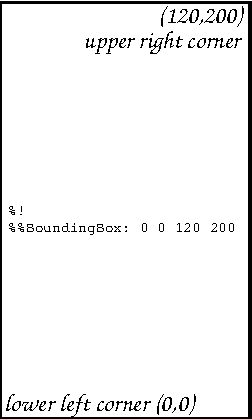
\includegraphics{fig1}
\end{figure}

\begin{figure}
\caption{HI}
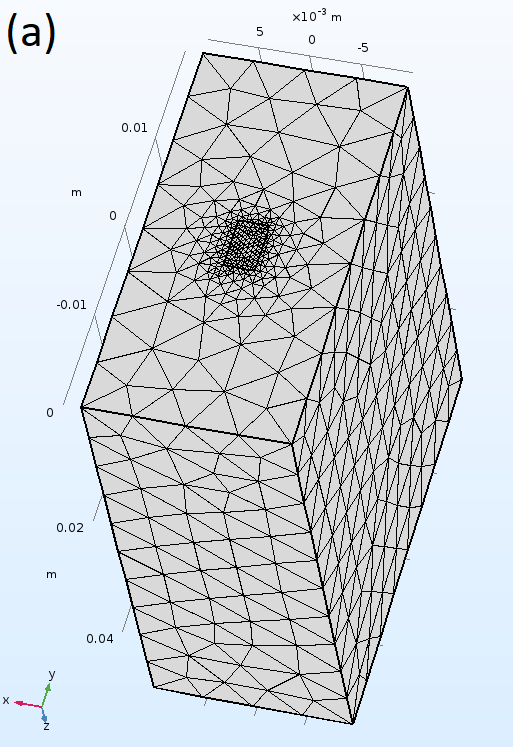
\includegraphics{images/bare_silicon.png}
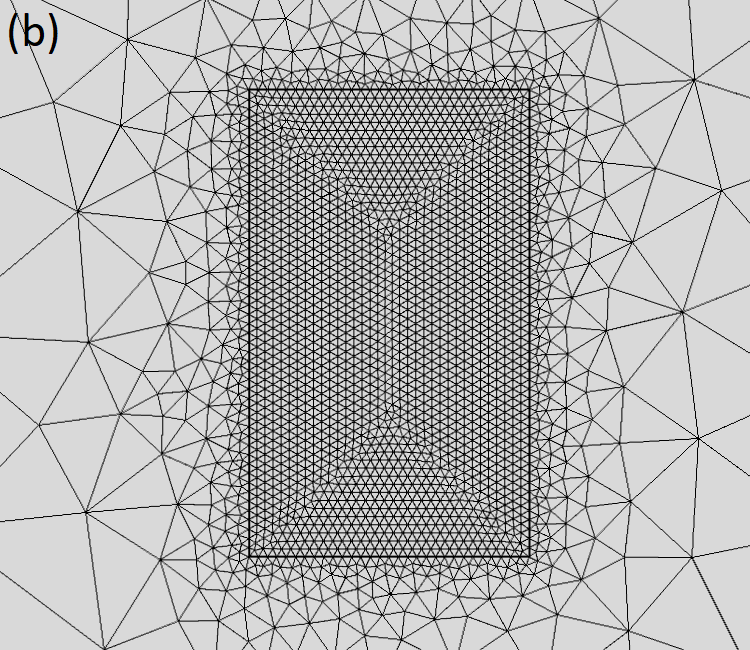
\includegraphics{images/incidence_mesh.png}
\label{fig:bare_silicon}
\end{figure}

\begin{figure}
\caption{HI}
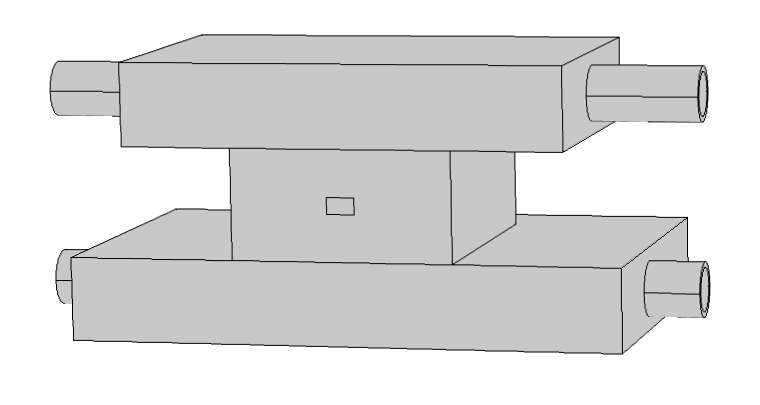
\includegraphics{images/nanomaxcomsol.png}
\label{fig:nanomaxcomsol}
\end{figure}


\begin{figure}
\caption{HI}
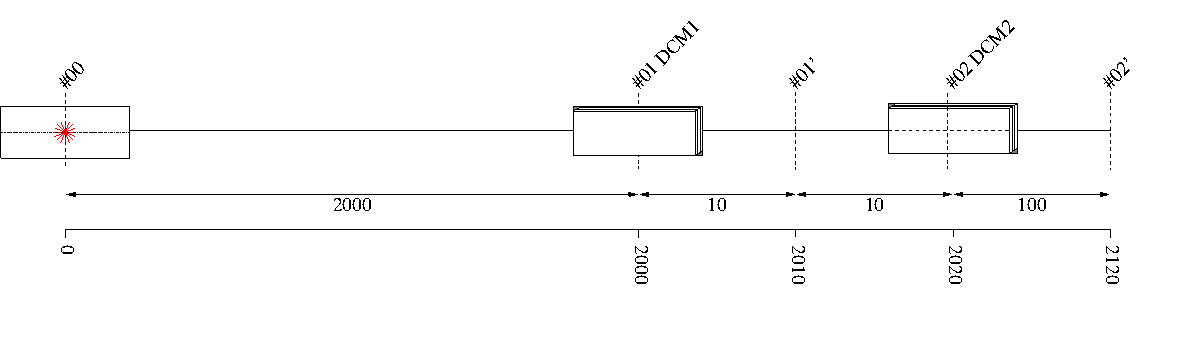
\includegraphics{images/gaussian_beamline.png}
\label{fig:dcmtracing}
\end{figure}


\begin{table}\label{gaussian}
\caption{Gaussian beam parameters}
\begin{tabular}{@{}llll@{}}
\toprule
Parameter       & Value         & Units     & Description                                          \\
\hline
x               & 0.005         & cm        & Gaussian $\sigma$ of horizontal intensity            \\
z               & 0.0005        & cm        & Gaussian $\sigma$ of vertical intensity              \\ 
y               & 0.0005        & cm        & Gaussian $\sigma$ of longitudinal intensity          \\
xp              & 50            & mrad      & Gaussian $\sigma$ of horizontal angular intensity    \\
zp              & 50            & mrad      & Gaussian $\sigma$ of horizontal angular intensity    \\

\end{tabular}
\end{table}

\begin{table}\label{ivubiomax}
\caption{Undulator Parameters}
\begin{tabular}{@{}llll@{}}
\toprule
Parameter       & Value         & Units     & Description                           \\
\hline
$\lambda$       & 1.8           & cm        & magnetic period length                \\
n               & 111           & 1         & number of magnetic periods            \\ 
$l$             & 1             & m         & magnetic length                       \\
$K$             & 2             & 1         & max K value                           \\
$\sigma_x$      & 40            & $\mu$m    & electron beam horizontal rms size     \\
$\sigma_z$      & 2             & $\mu$m    & electron beam vertical rms size       \\
$\epsilon_x$    & 3.3e-08       & cm-rad    & electron beam horizontal emittance    \\
$\epsilon_z$    & 8e-10         & cm-rad    & electron beam vertical emittance      \\
I               & 500           & mA        & electron beam current                 \\
E               & 3             & GeV       & electron energy                       \\
\end{tabular}
\end{table}

\begin{table}\label{ivwbalder}
\caption{Wiggler Parameters}
\begin{tabular}{@{}llll@{}}
\toprule
Parameter       & Value         & Units     & Description                           \\
\hline
$\lambda$       & 5             & cm        & magnetic period length                \\
n               & 40            & 1         & number of magnetic periods            \\ 
$l$             & 1             & m         & magnetic length                       \\
$K$             & 9             & 1         & max K value                           \\
$\sigma_x$      & 50            & $\mu$m    & electron beam horizontal rms size     \\
$\sigma_z$      & 2             & $\mu$m    & electron beam vertical rms size       \\
$\epsilon_x$    & 3.3e-08       & cm-rad    & electron beam horizontal emittance    \\
$\epsilon_z$    & 8e-10         & cm-rad    & electron beam vertical emittance      \\
I               & 500           & mA        & electron beam current                 \\
E               & 3             & GeV       & electron energy                       \\
\end{tabular}
\end{table}


\begin{figure}
\caption{HI}
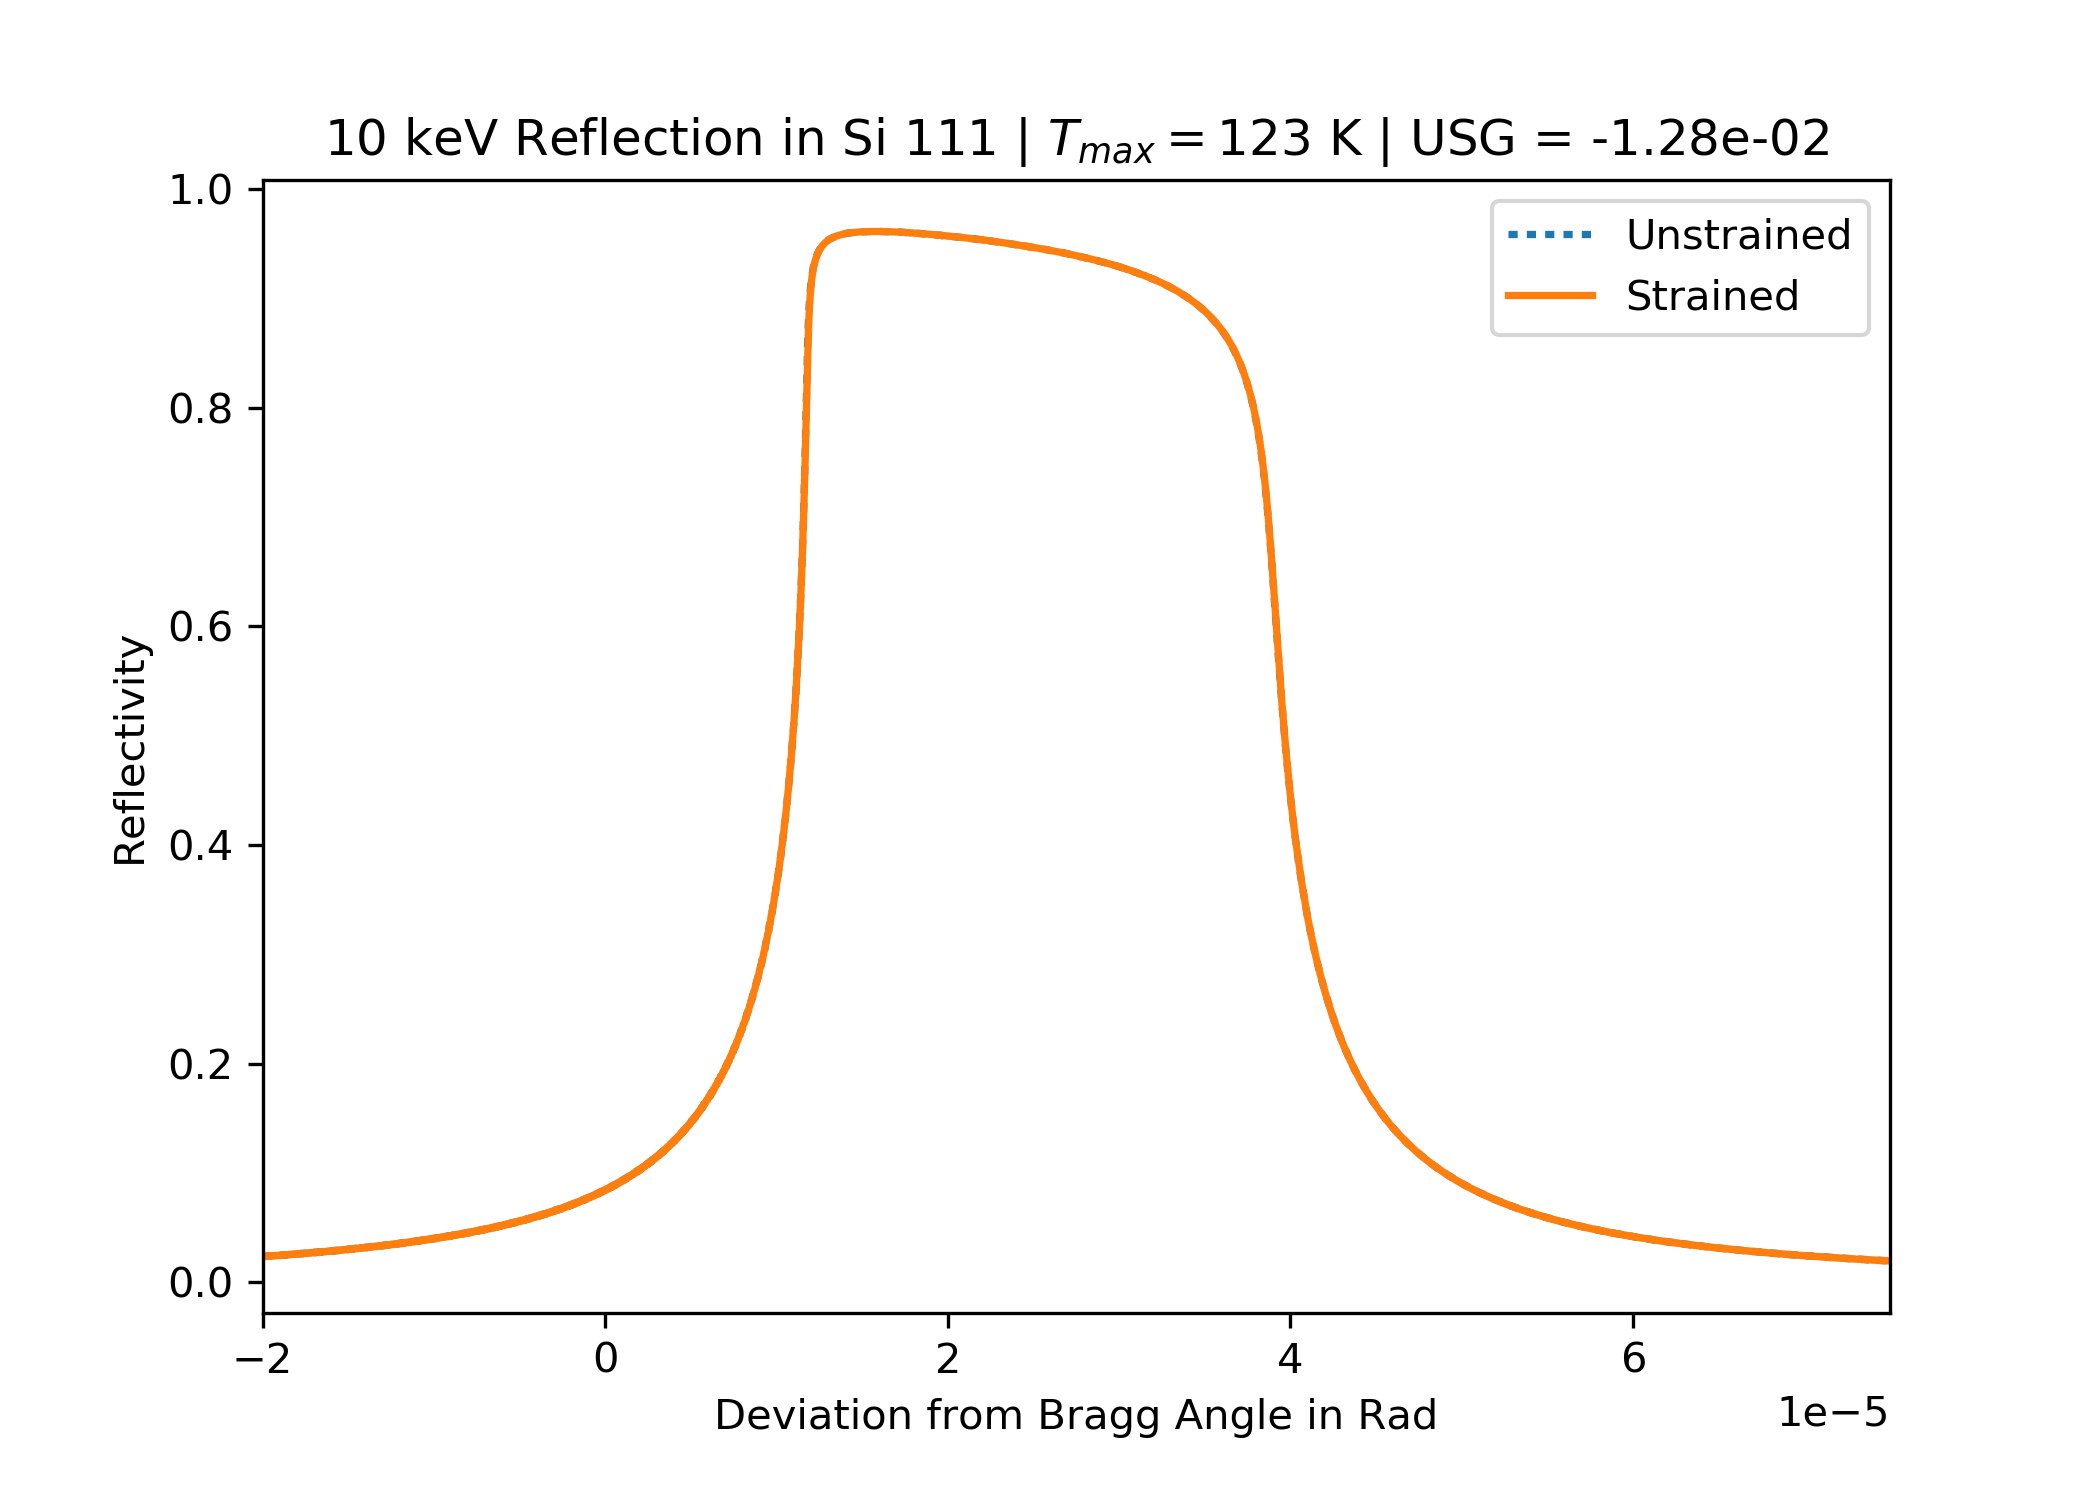
\includegraphics{images/111_10keV_4.png}
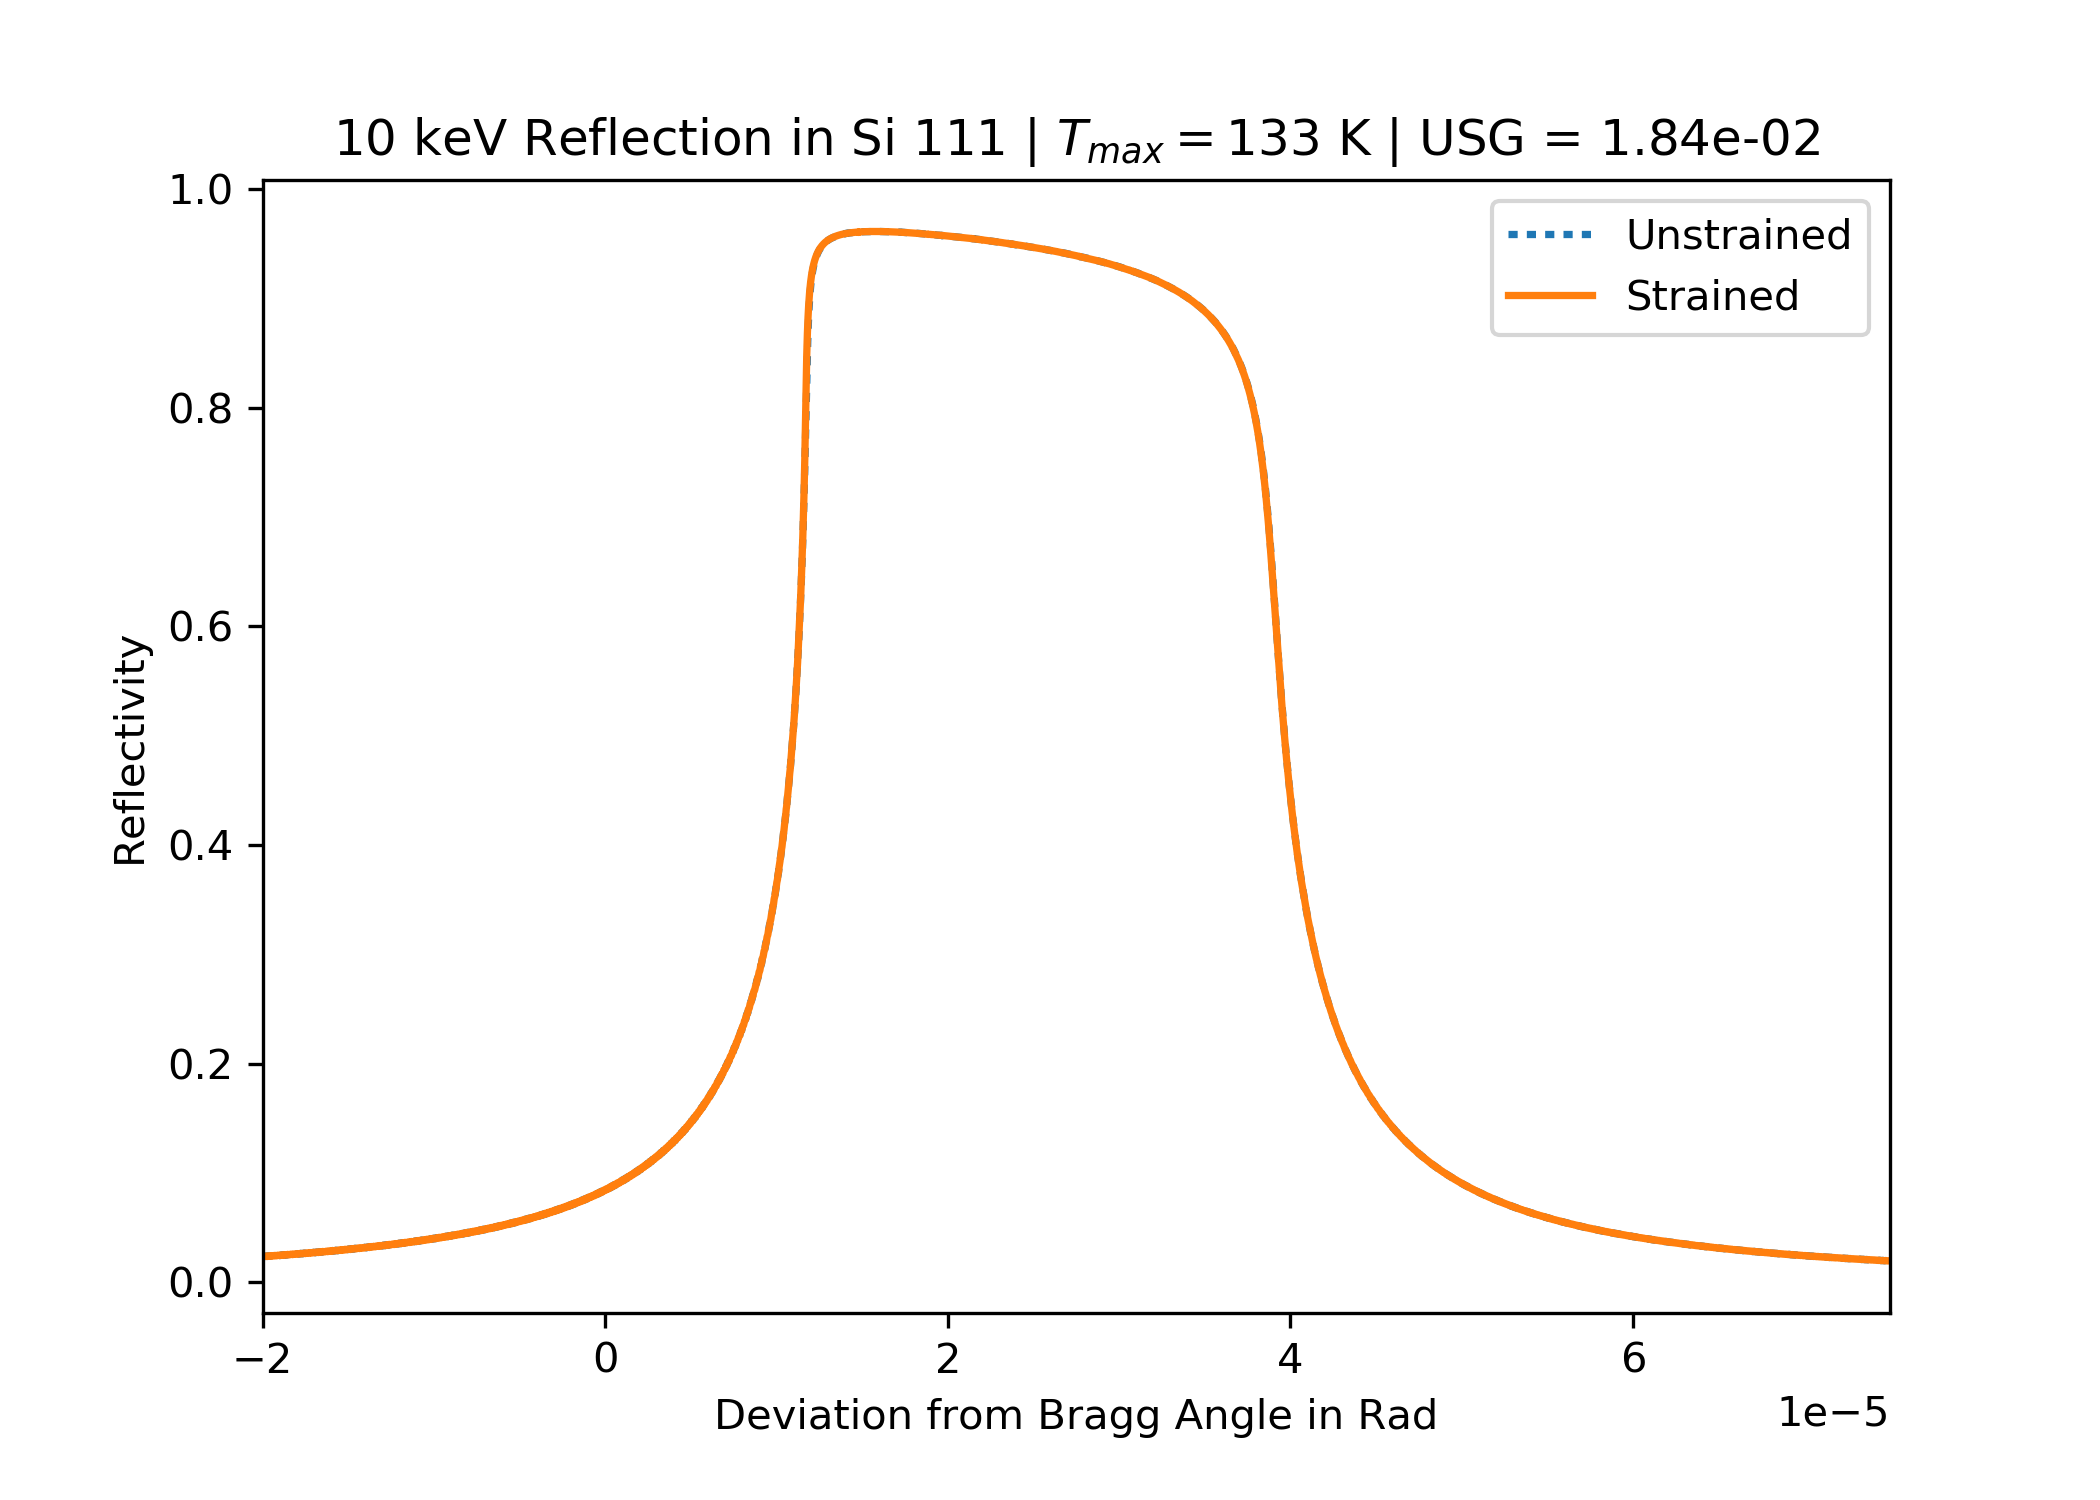
\includegraphics{images/111_10keV_5.png}
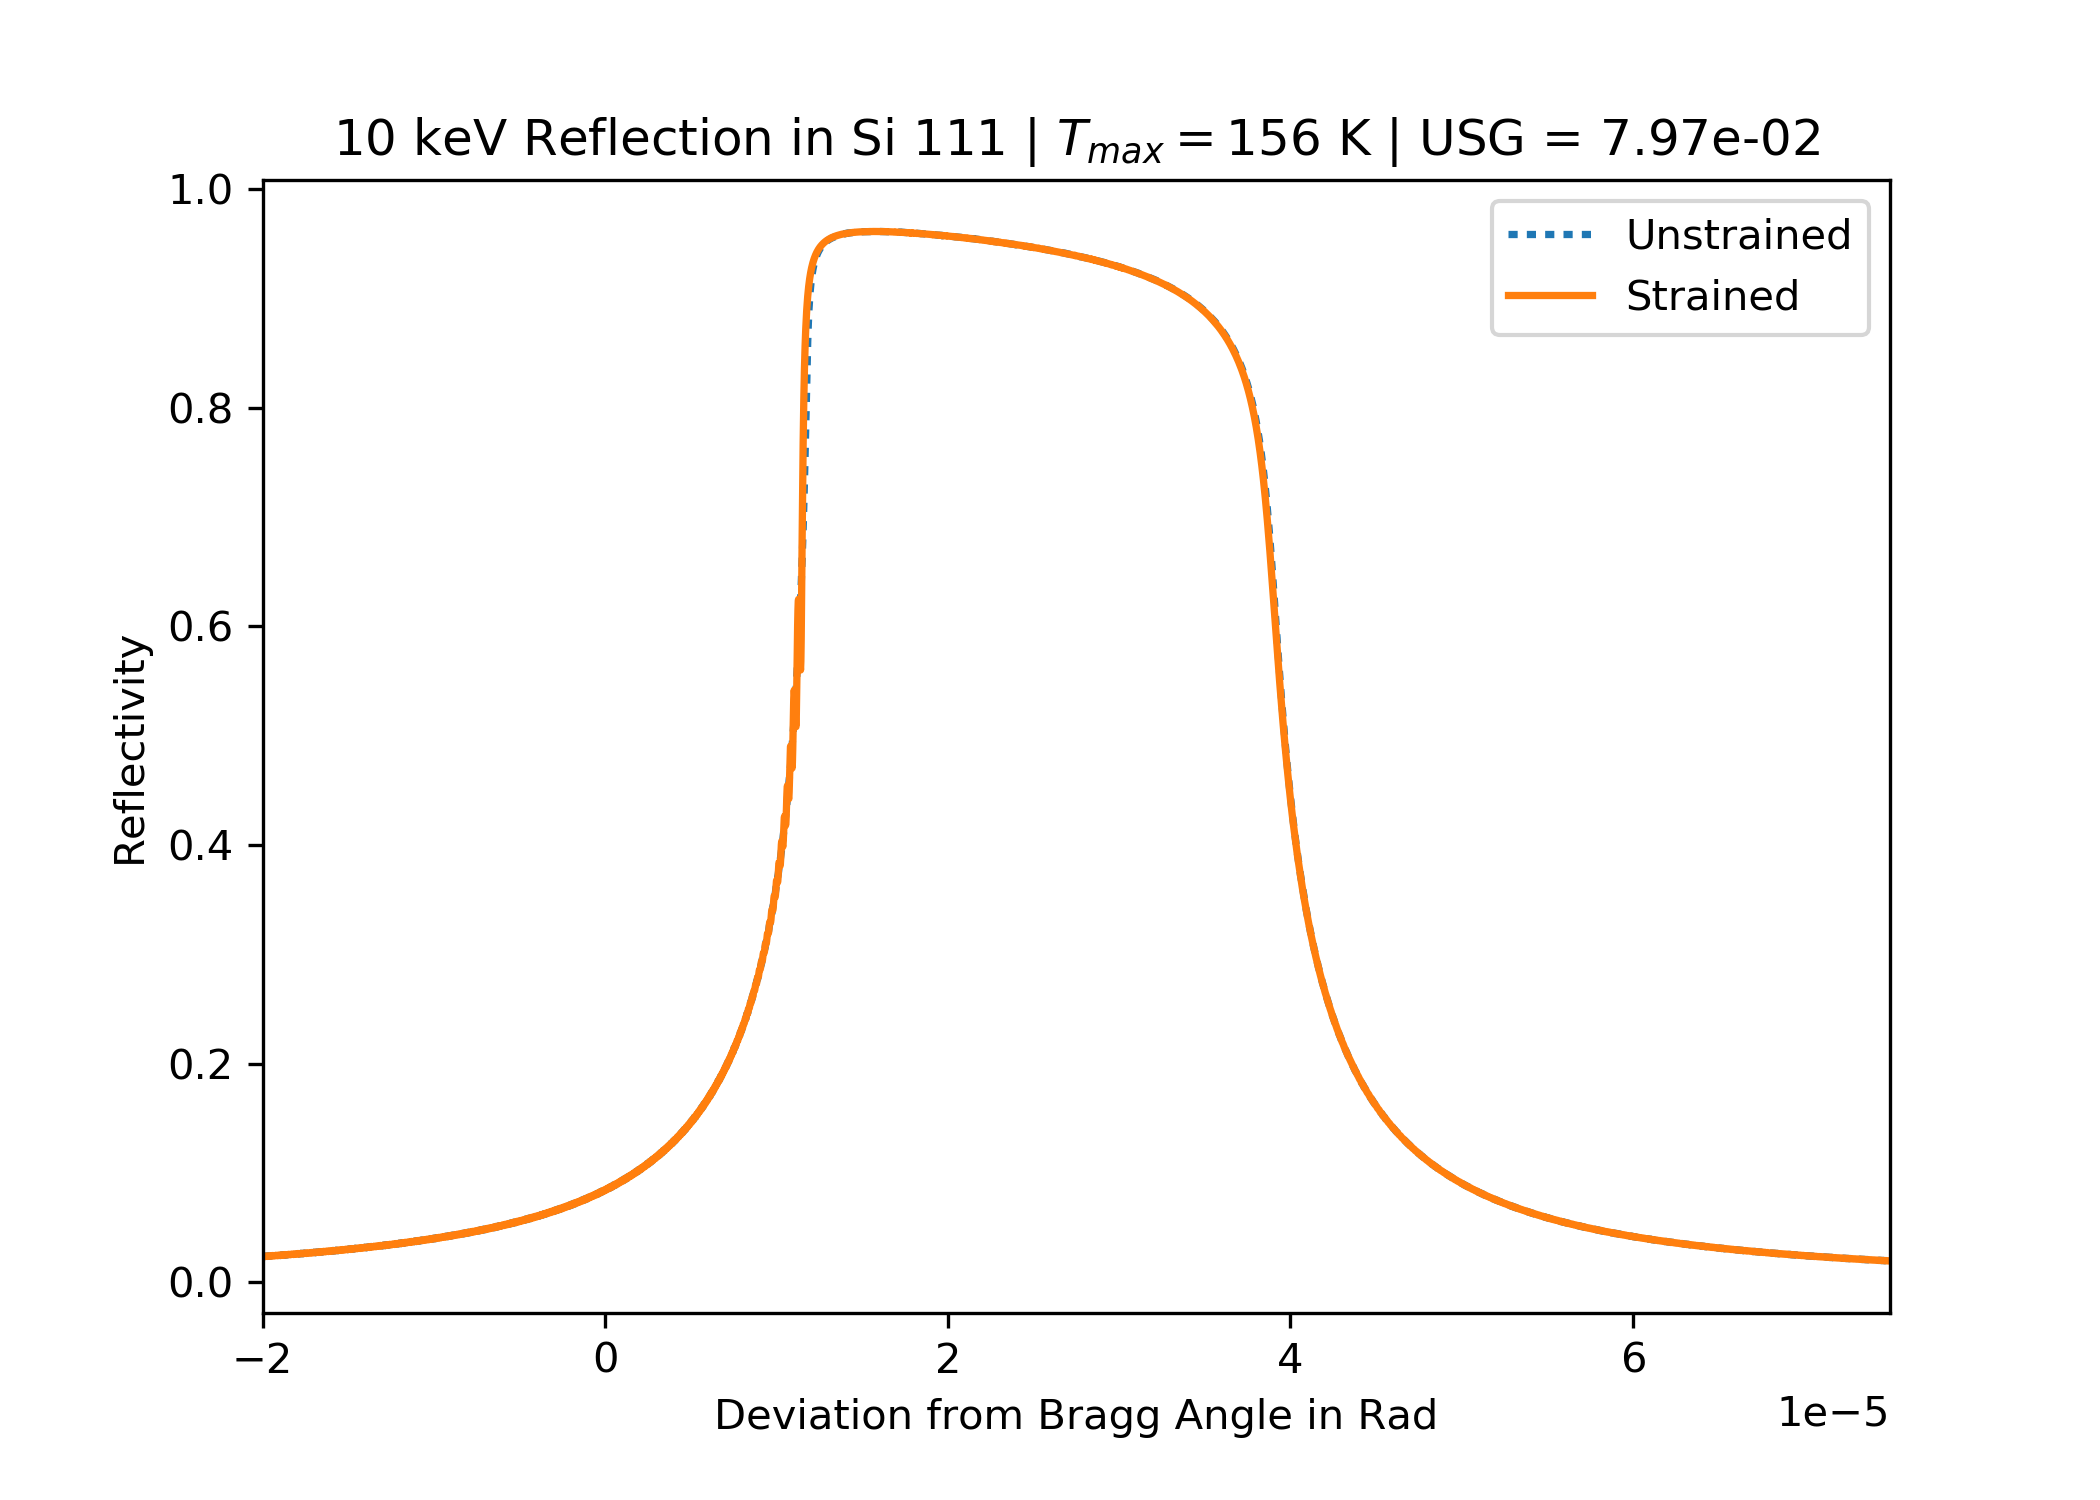
\includegraphics{images/111_10keV_7.png}
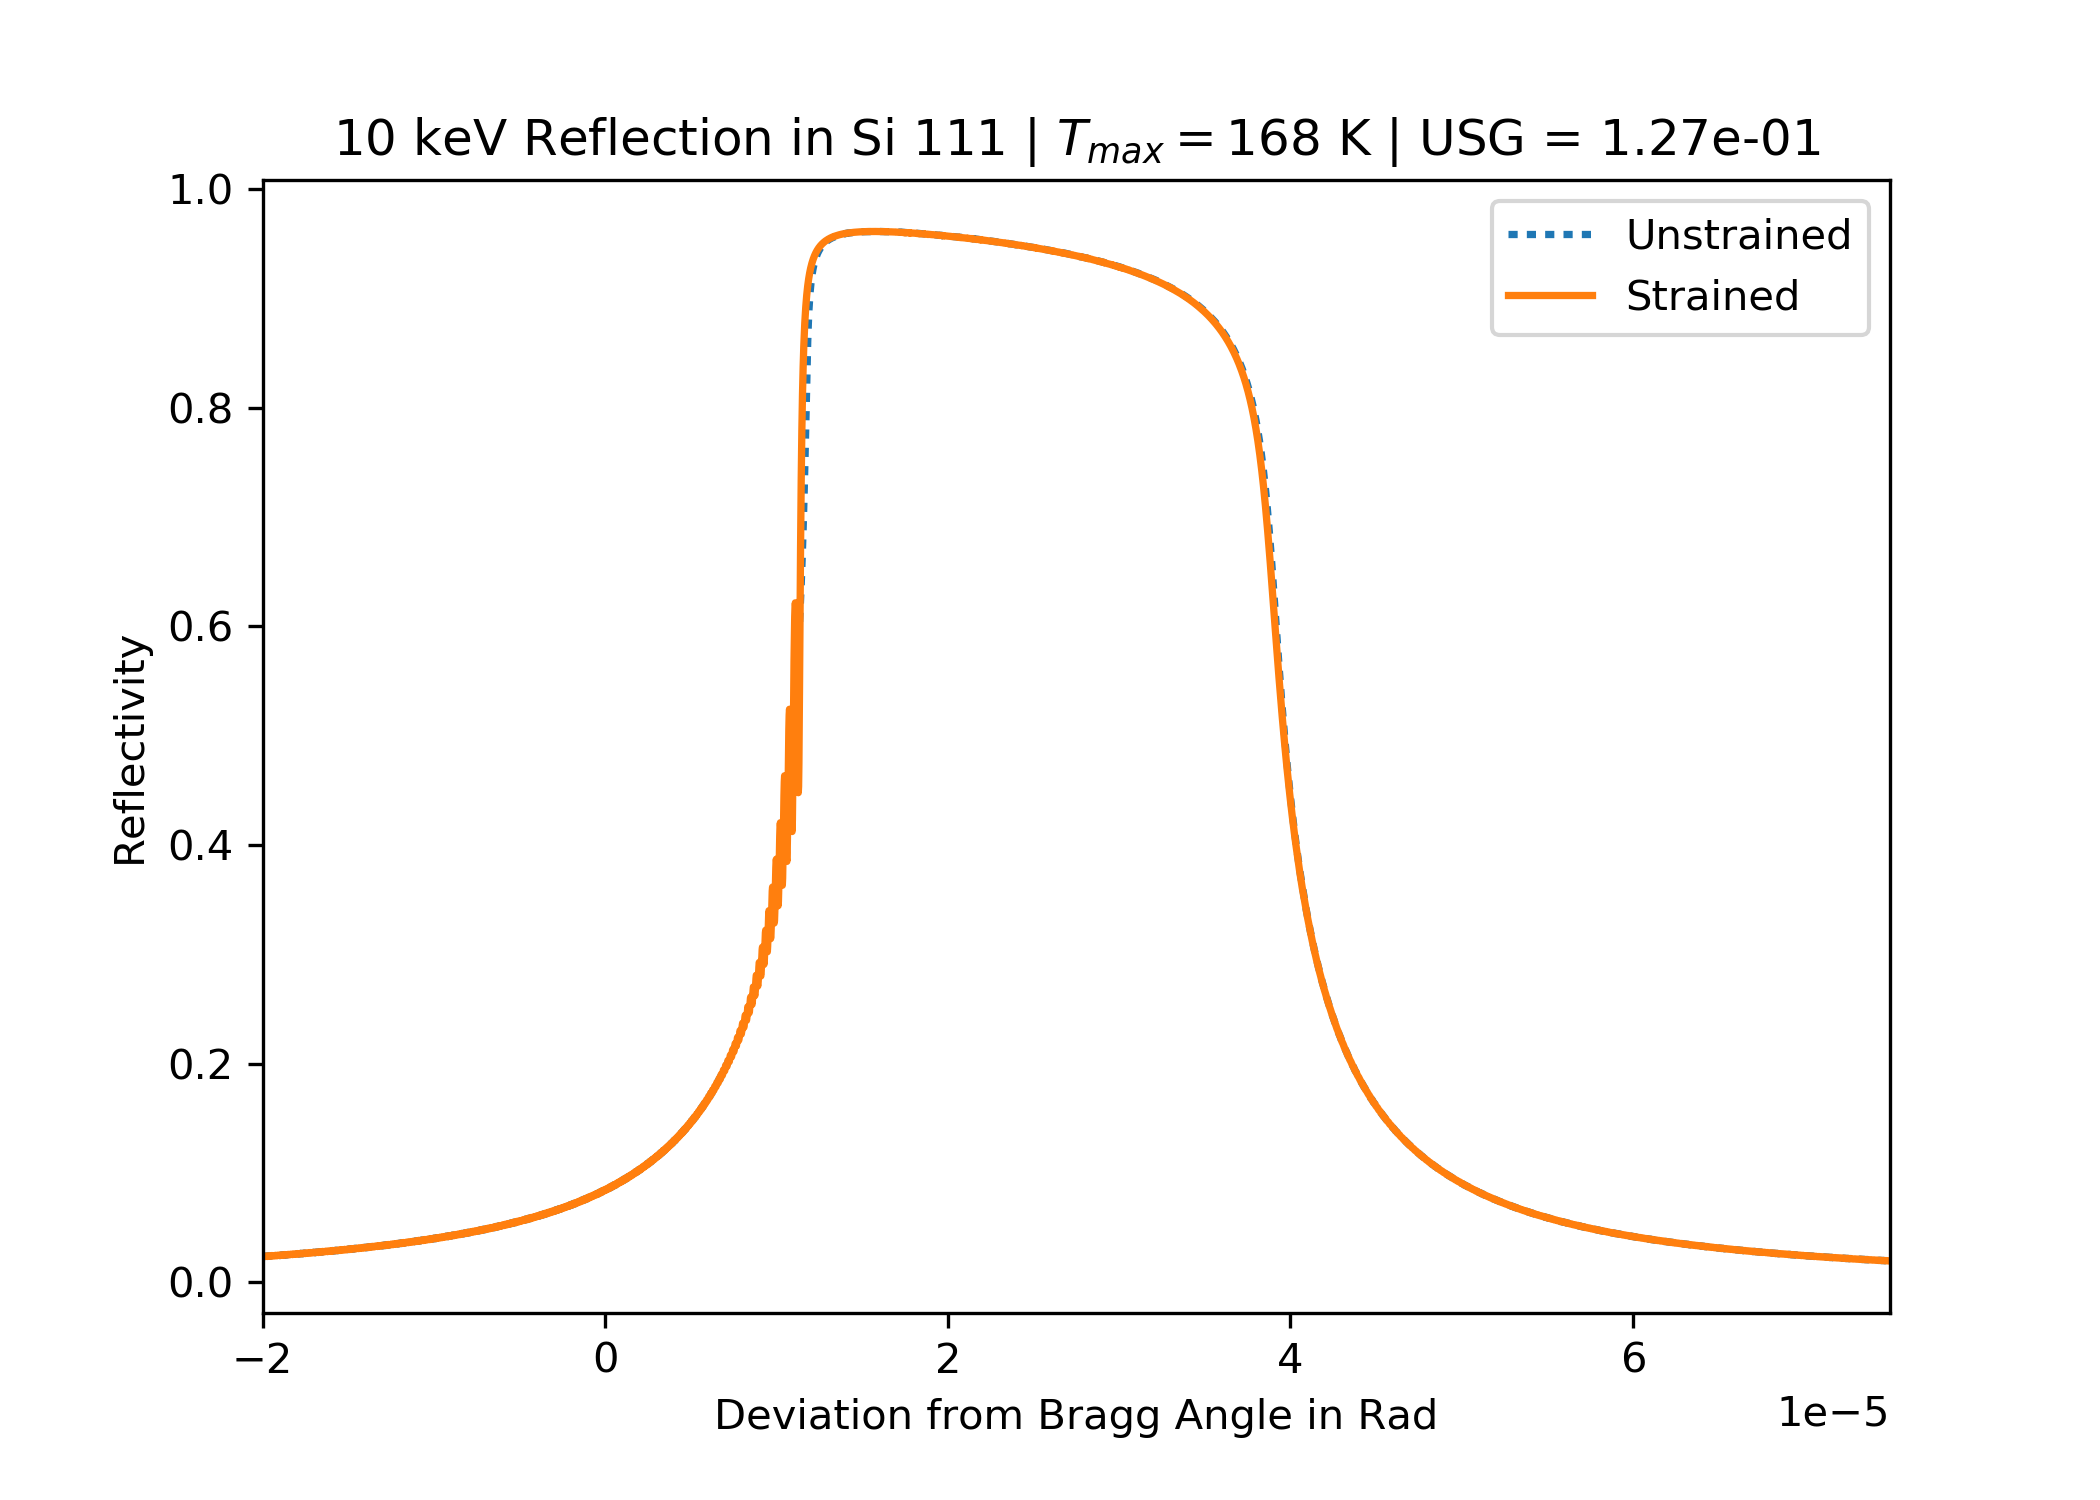
\includegraphics{images/111_10keV_8.png}
\label{fig:111usg10kev}
\end{figure}

\begin{figure}
\caption{HI}
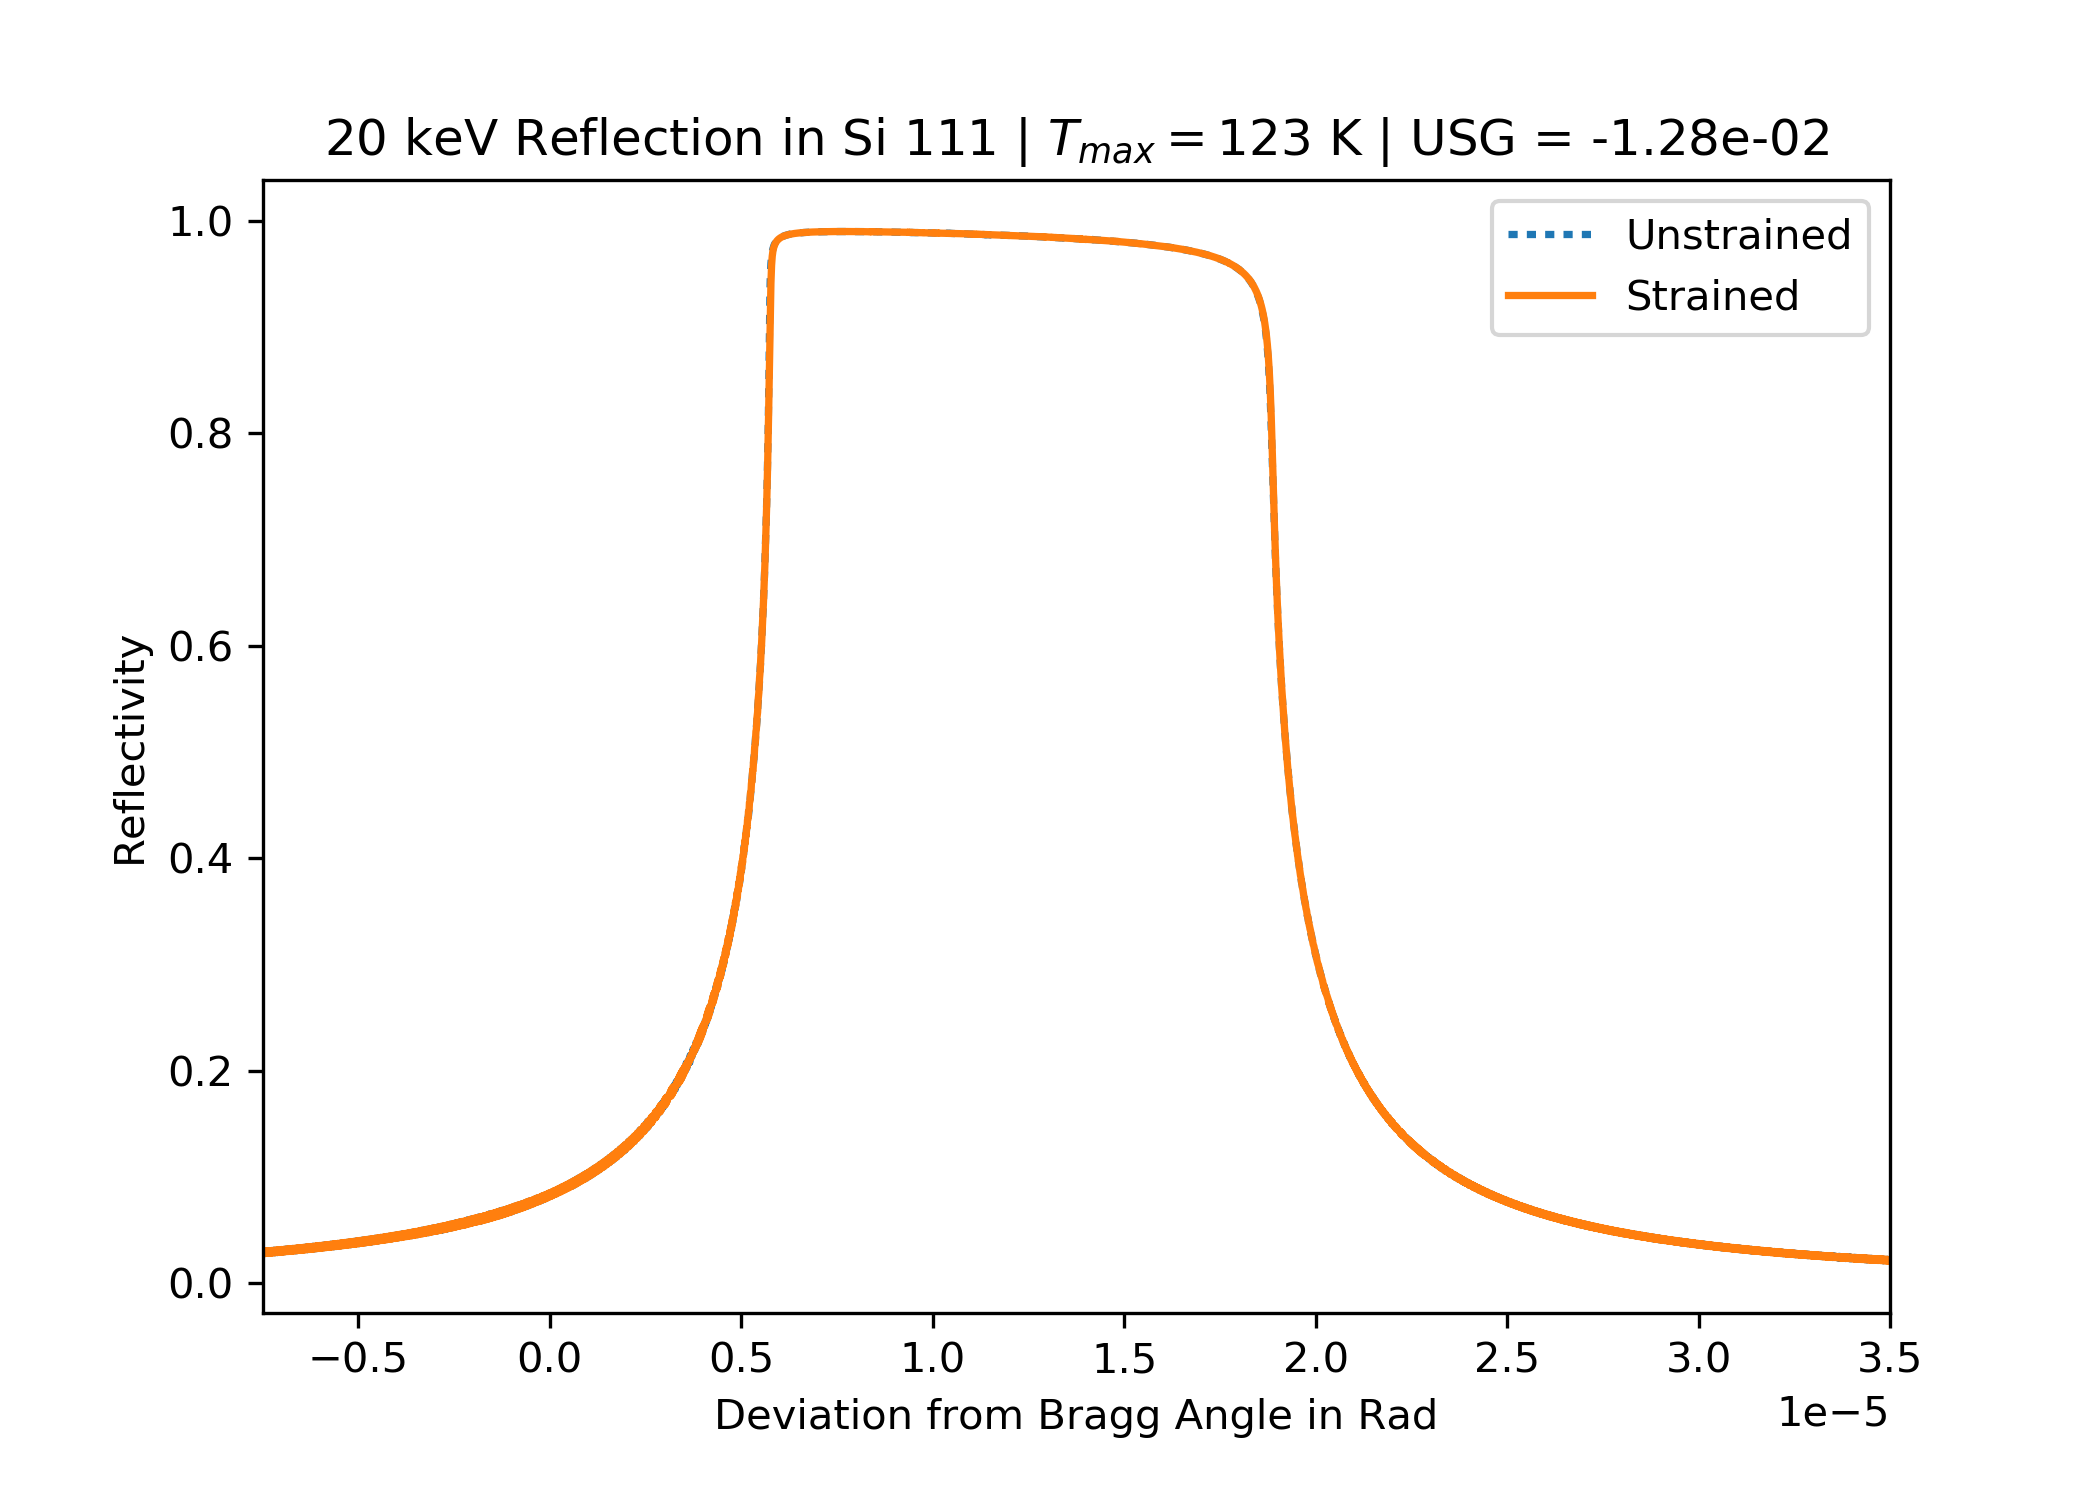
\includegraphics{images/111_20keV_4.png}
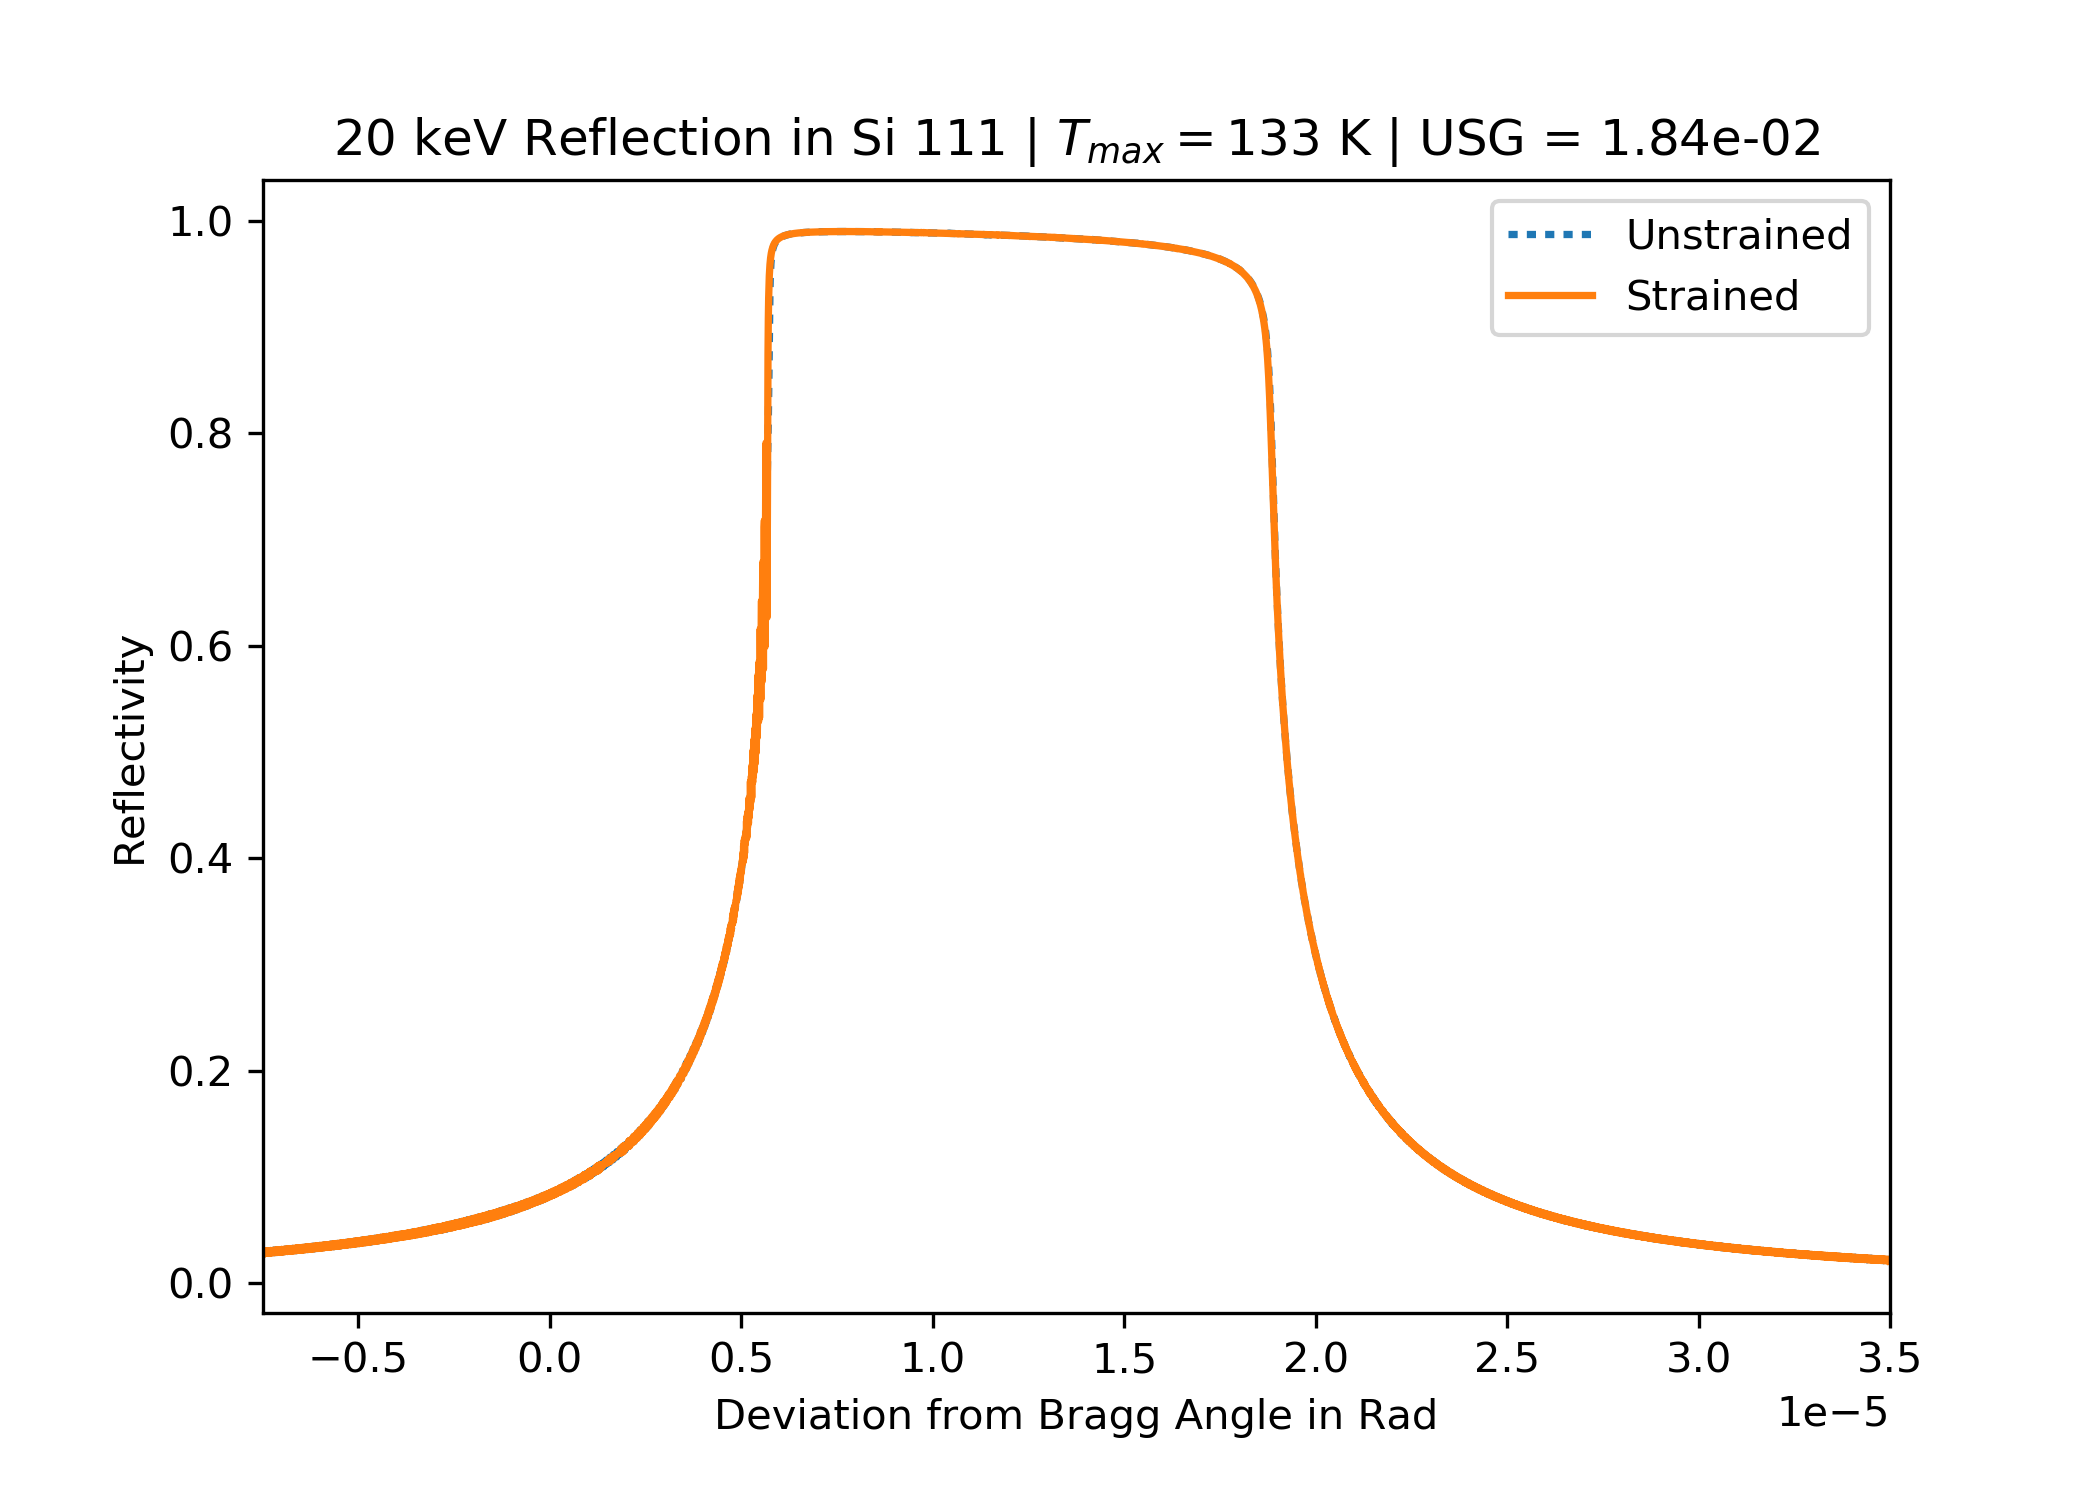
\includegraphics{images/111_20keV_5.png}
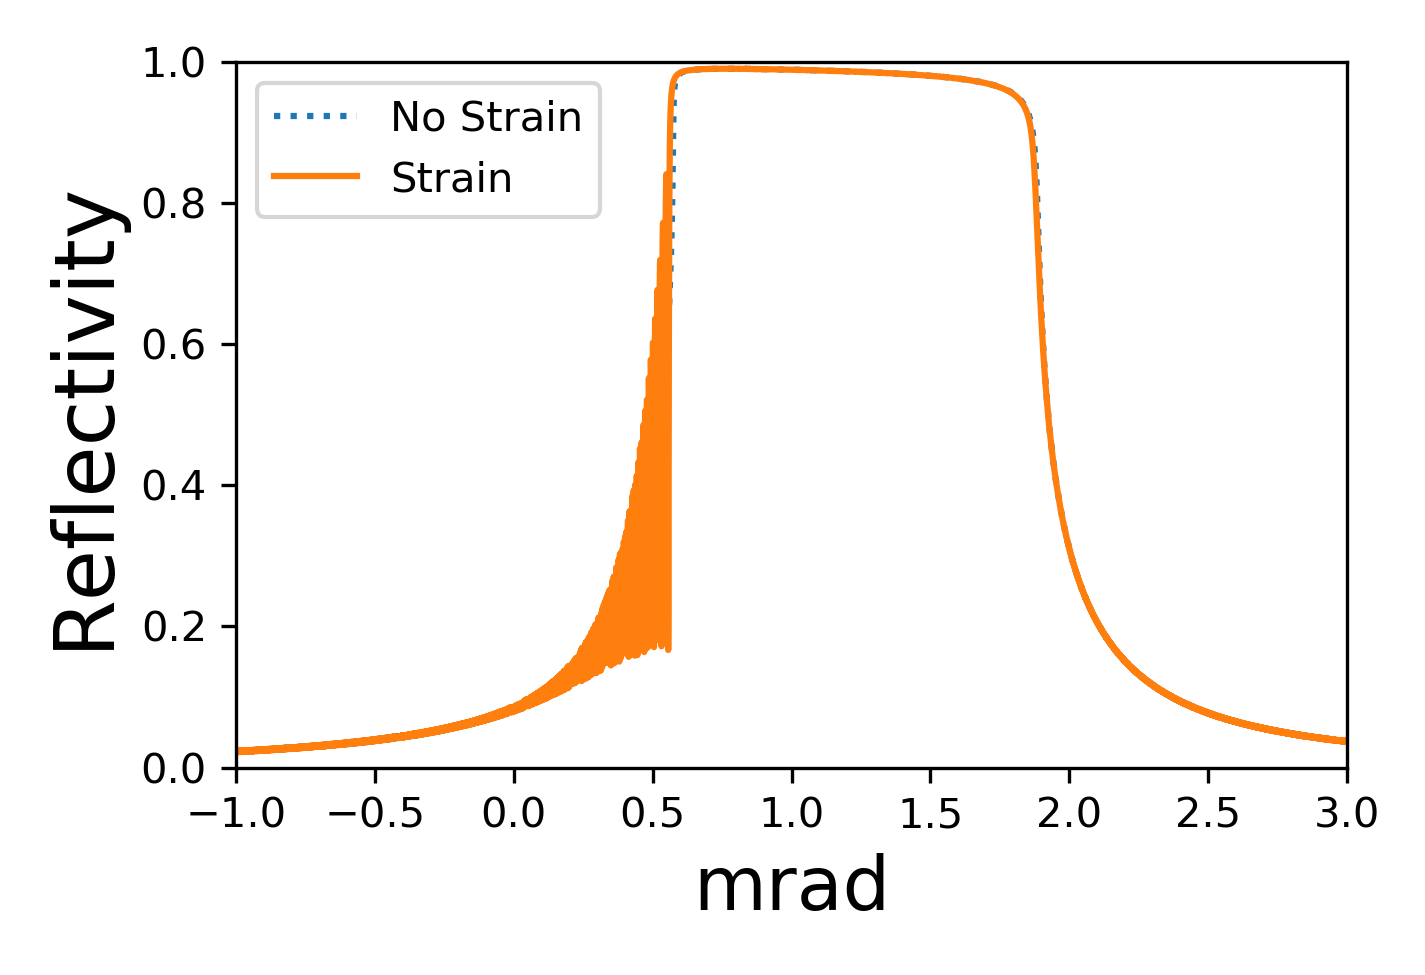
\includegraphics{images/111_20keV_7.png}
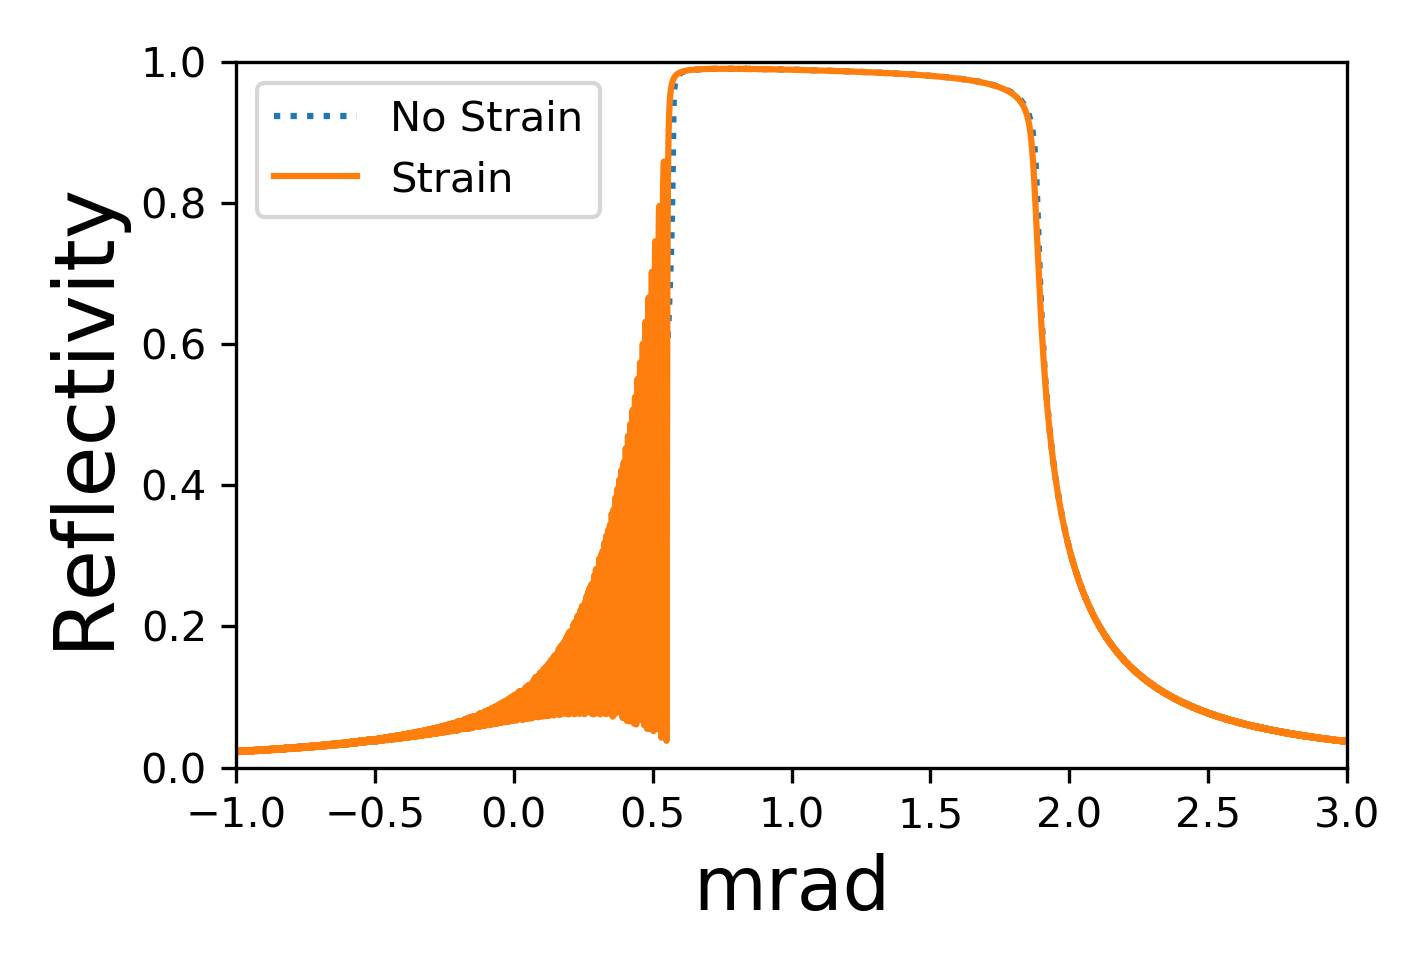
\includegraphics{images/111_20keV_8.png}
\label{fig:111usg20kev}
\end{figure}

\begin{figure}
\caption{HI}
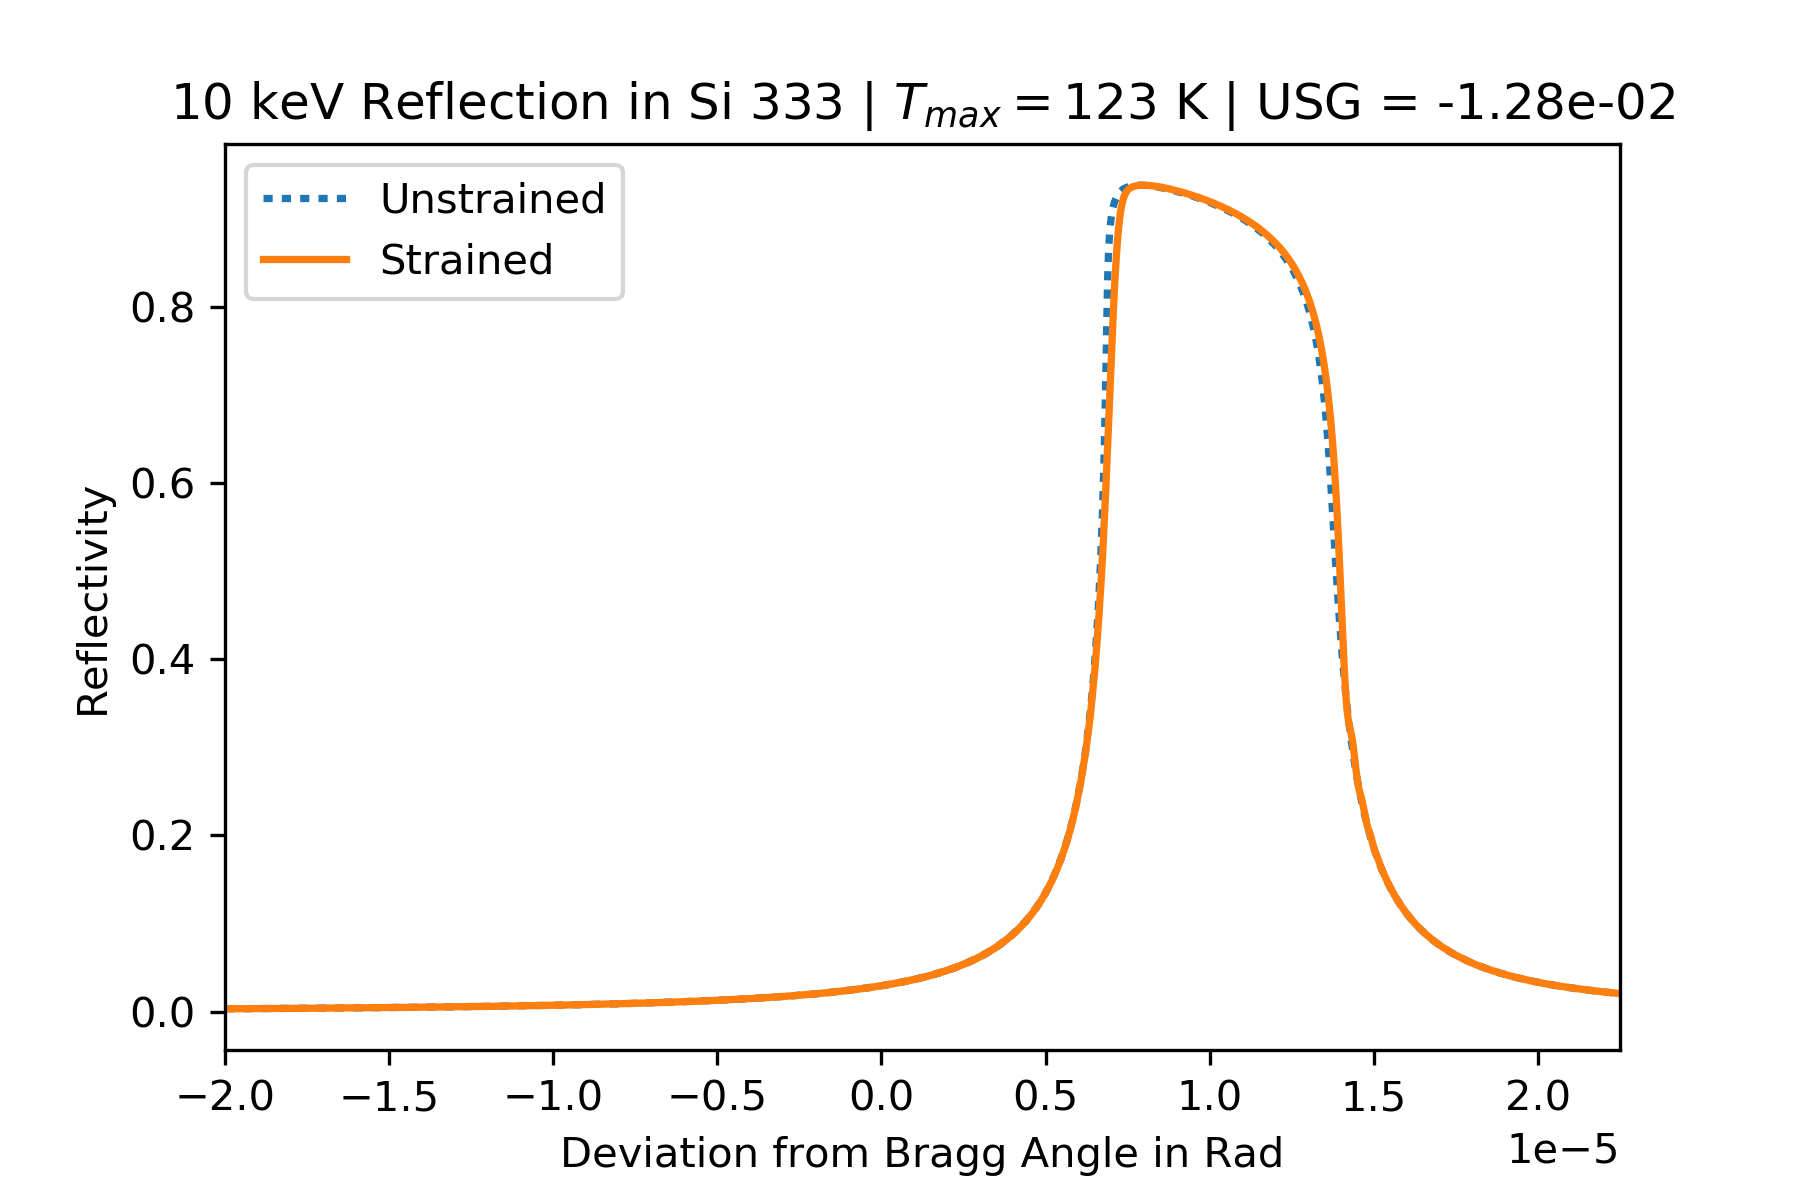
\includegraphics{images/333_10keV_4.png}
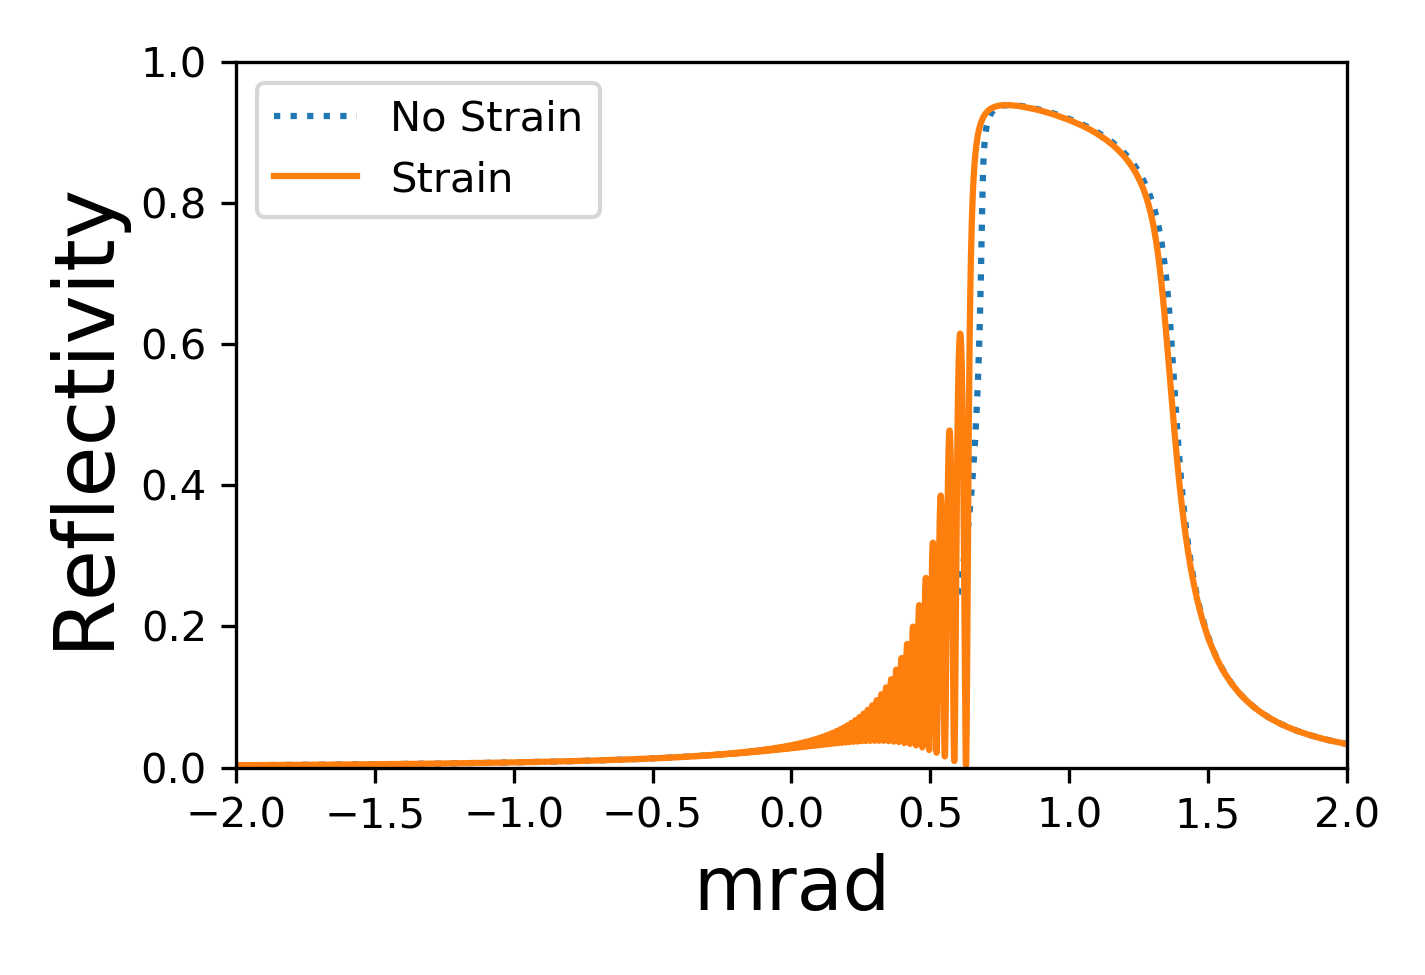
\includegraphics{images/333_10keV_5.png}
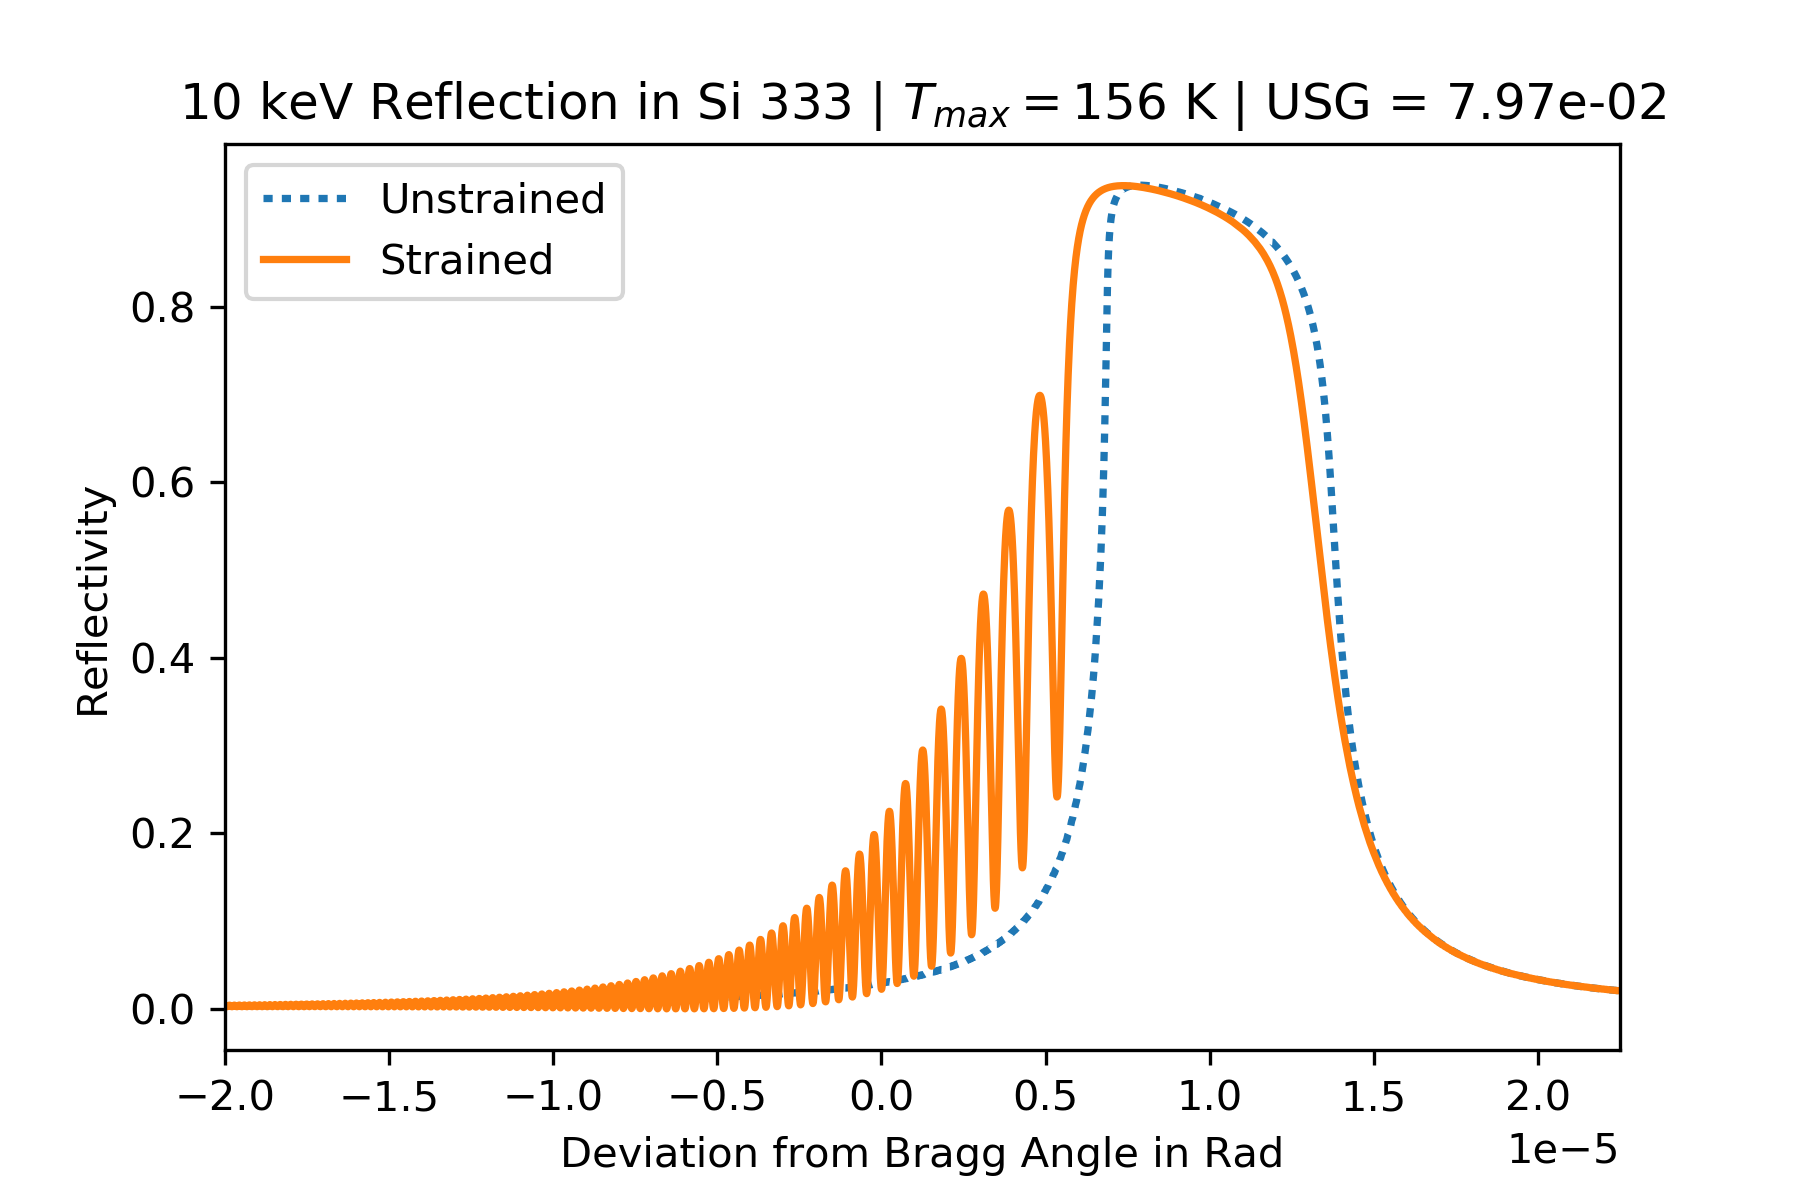
\includegraphics{images/333_10keV_7.png}
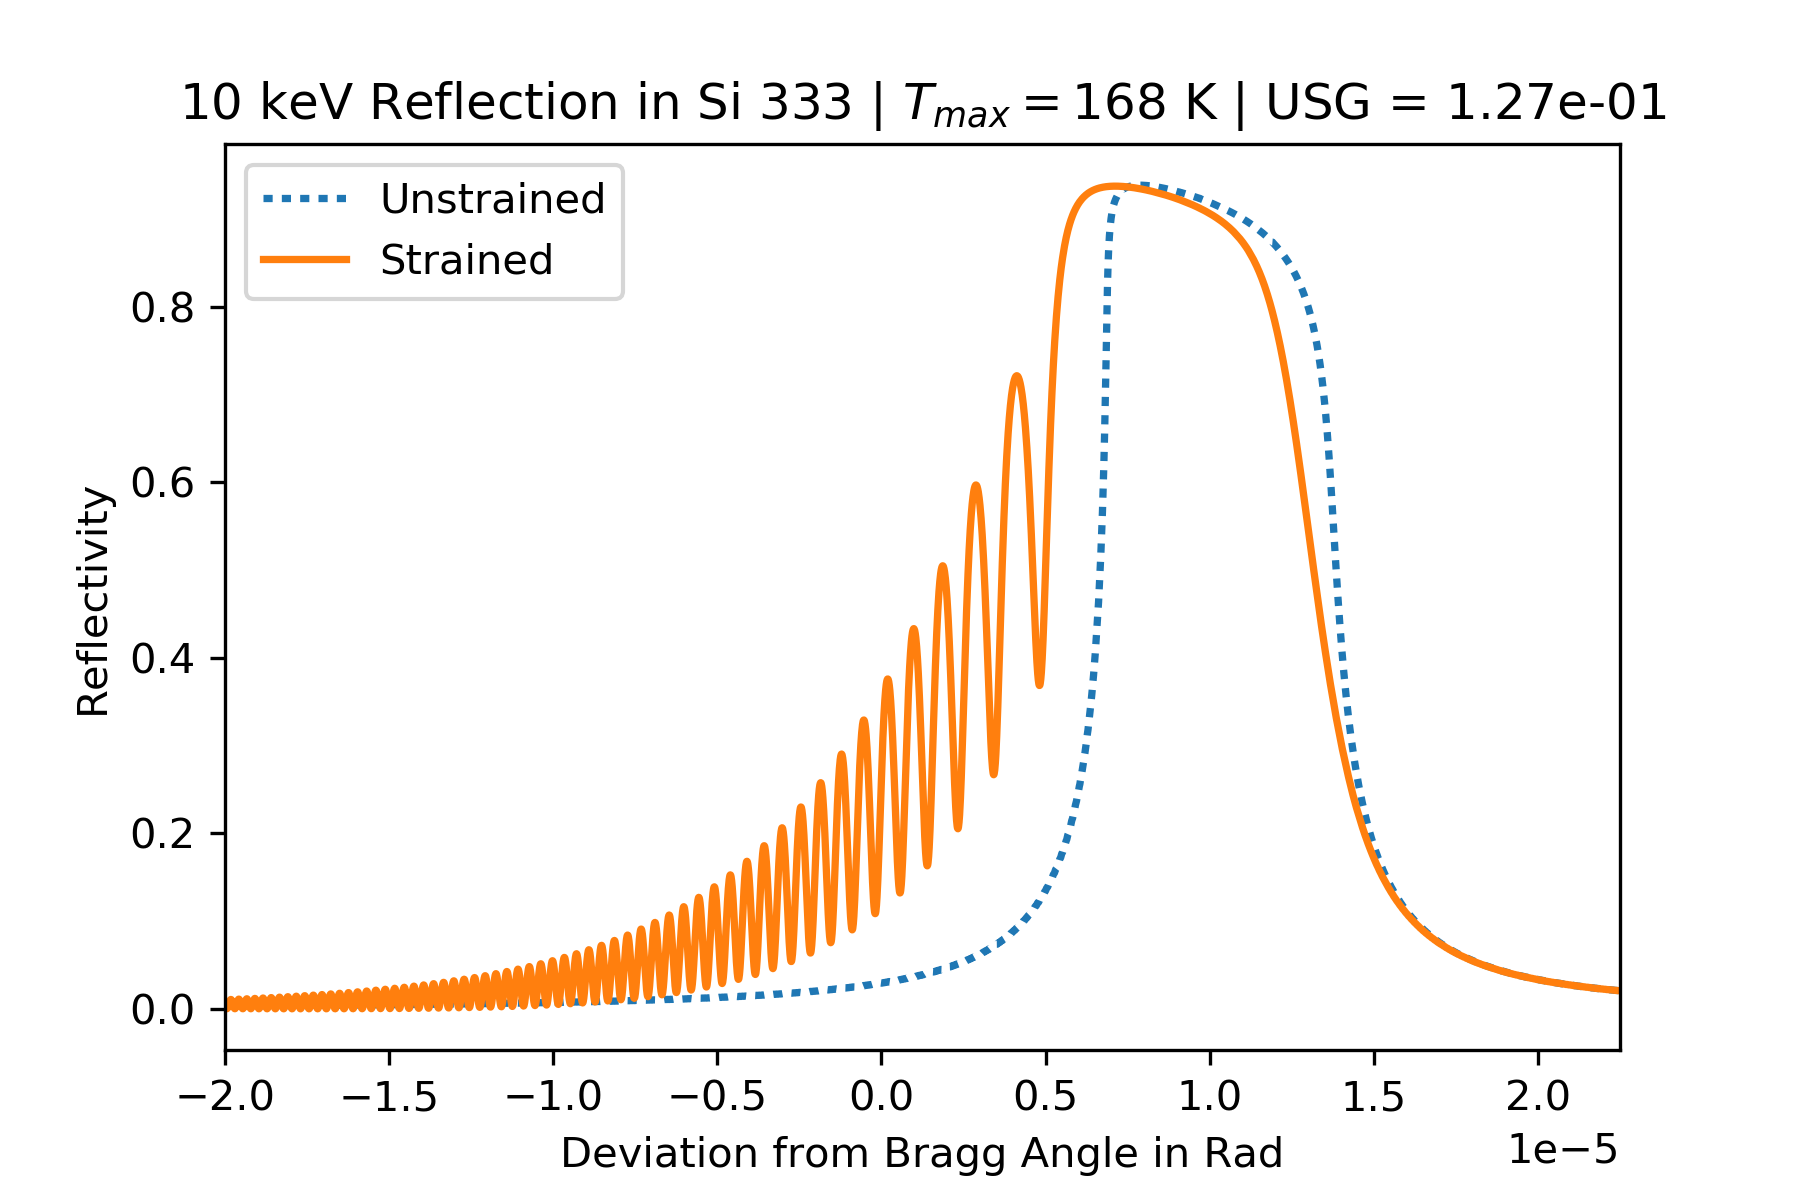
\includegraphics{images/333_10keV_8.png}
\label{fig:333usg10kev}
\end{figure}

\begin{figure}
\caption{HI}
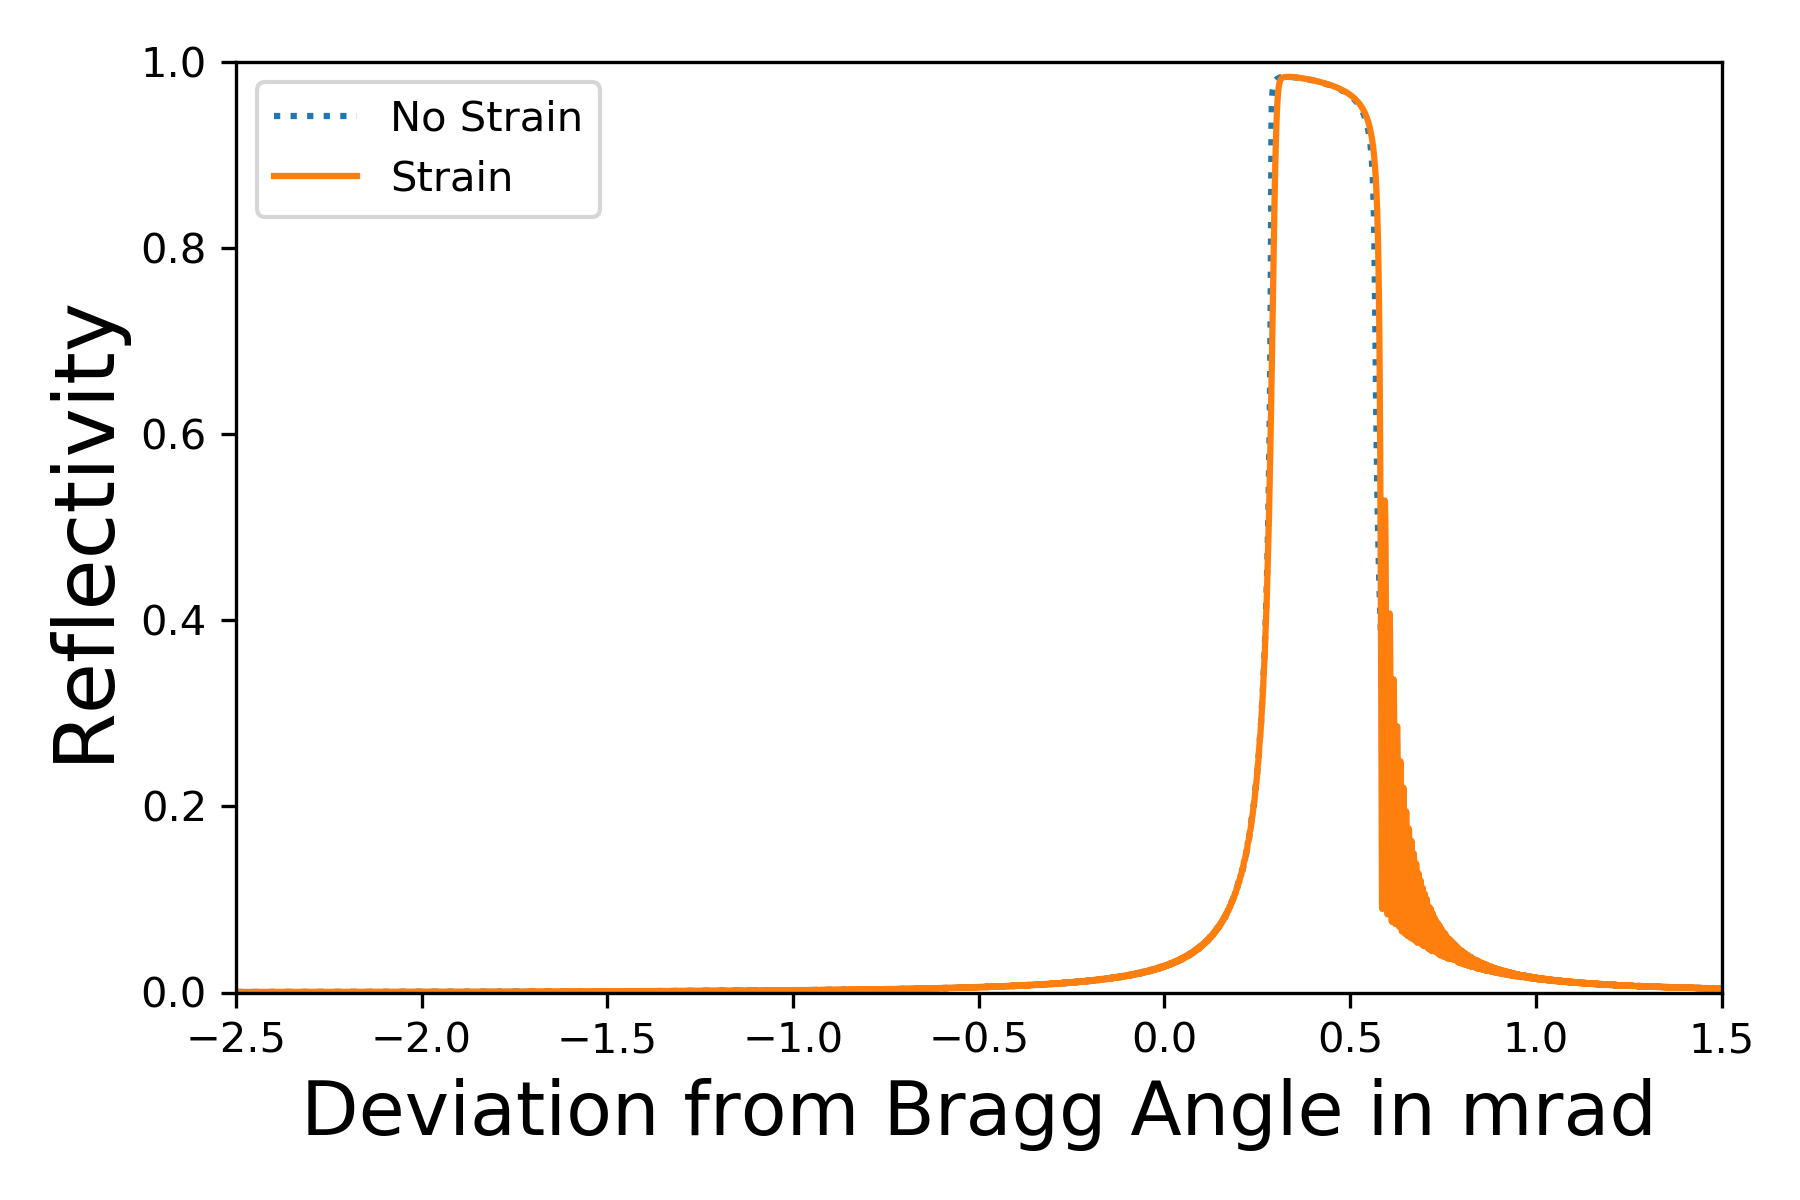
\includegraphics{images/333_20keV_4.png}
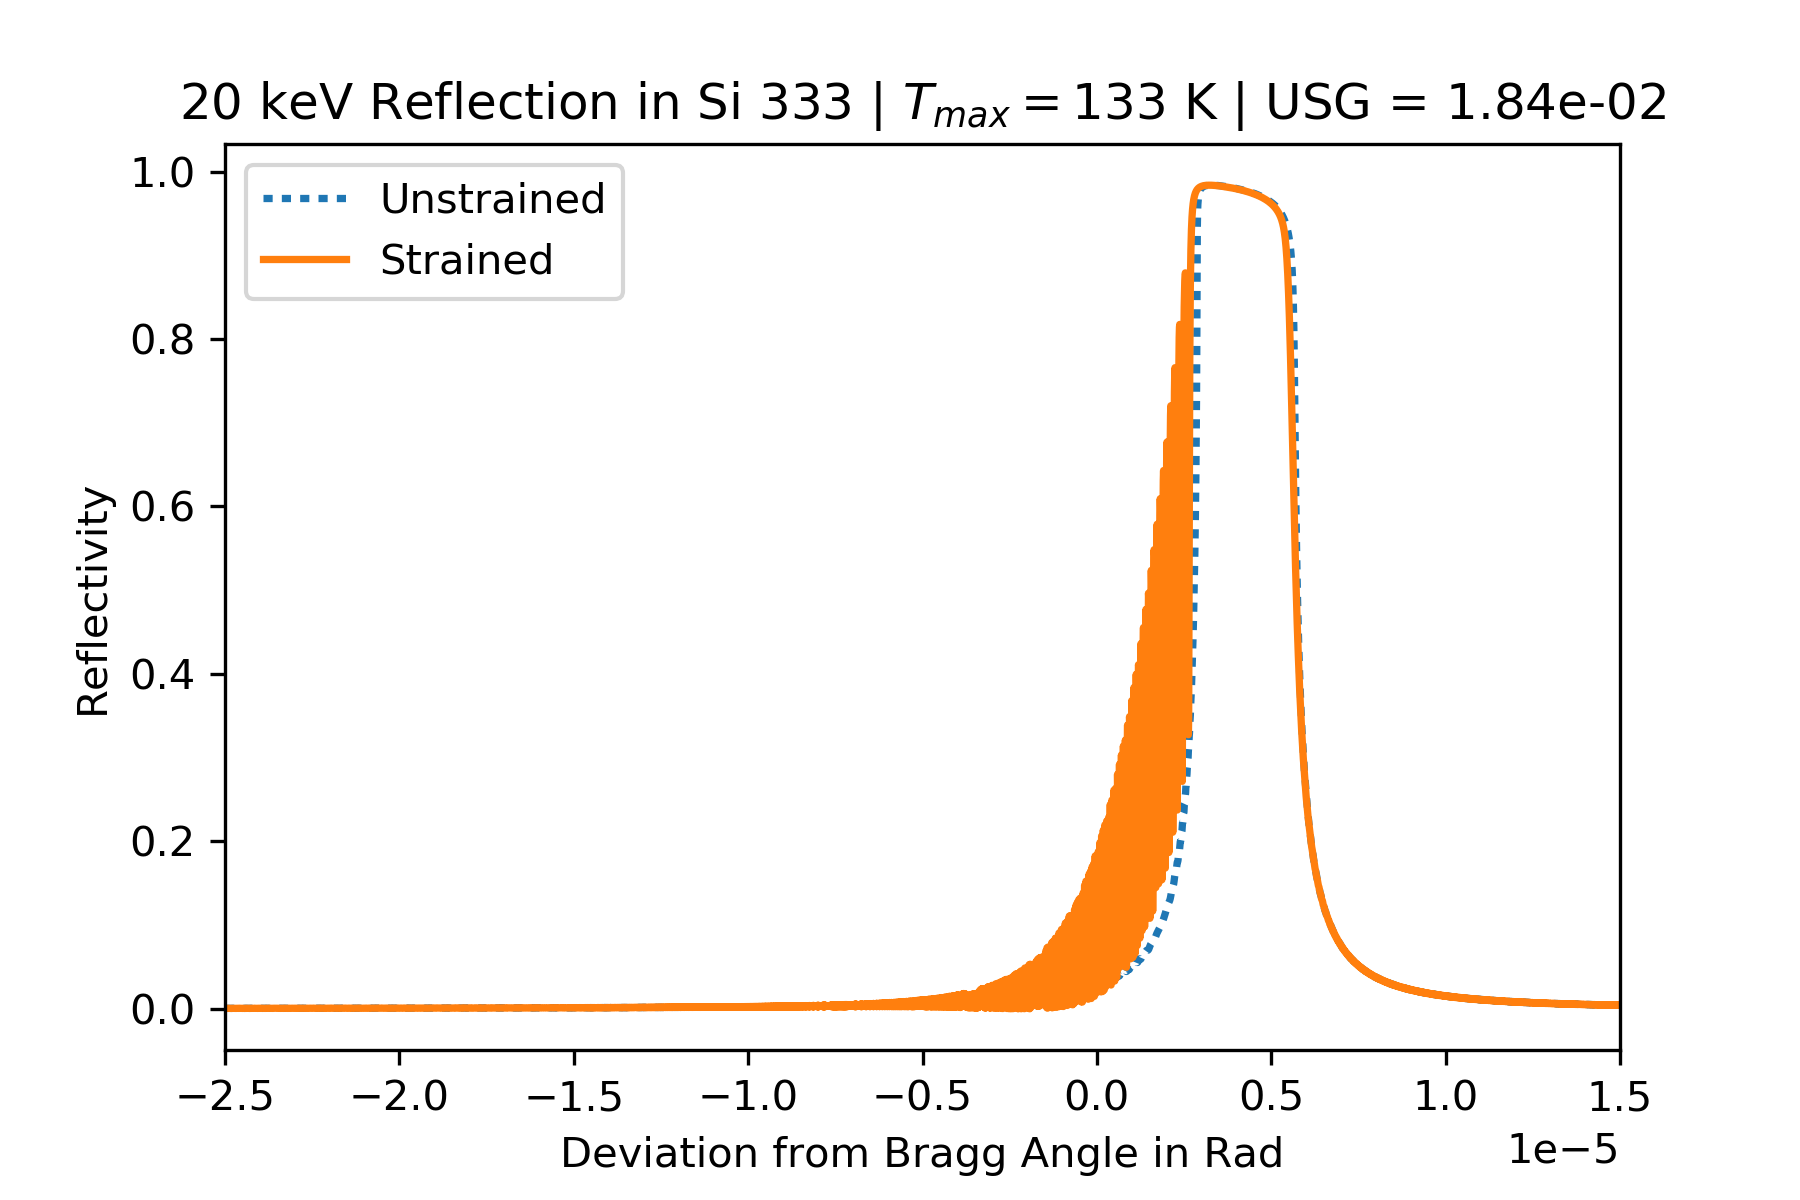
\includegraphics{images/333_20keV_5.png}
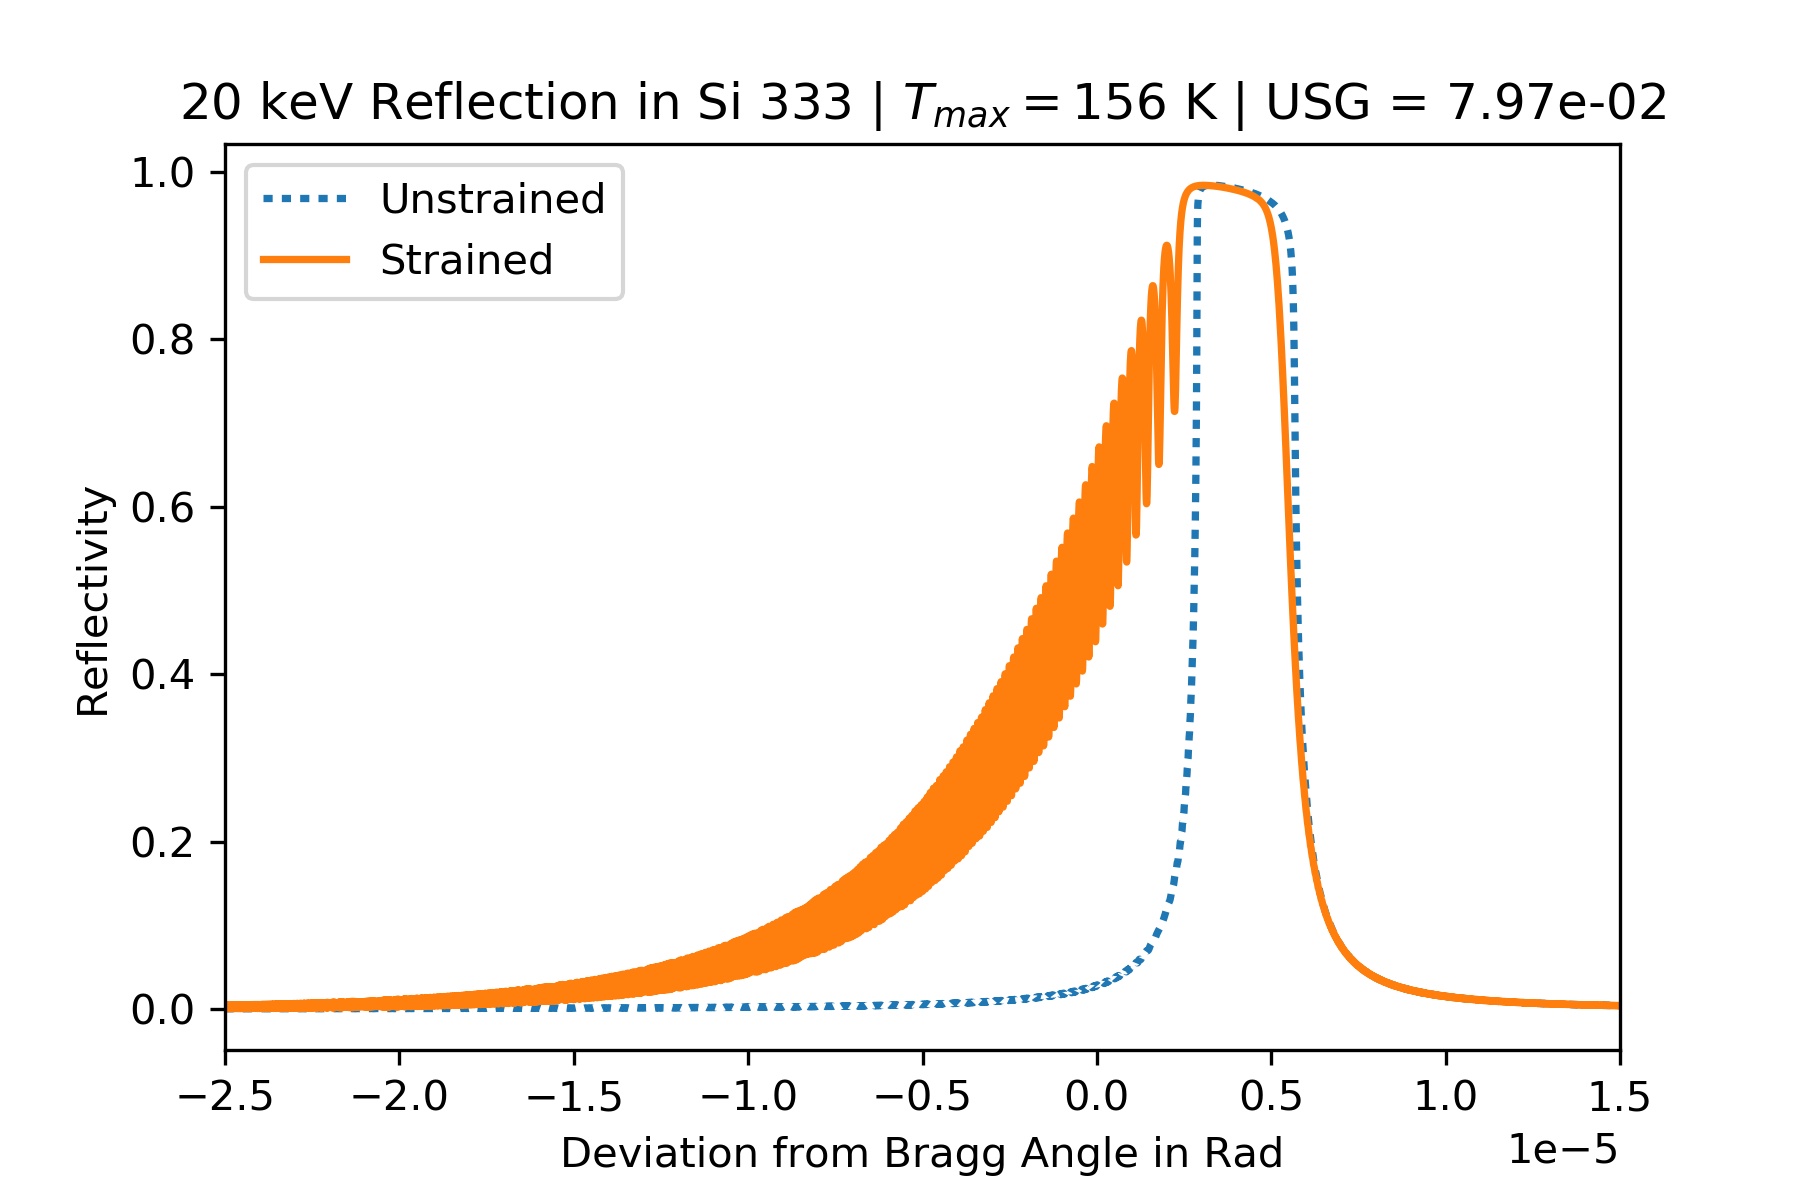
\includegraphics{images/333_20keV_7.png}
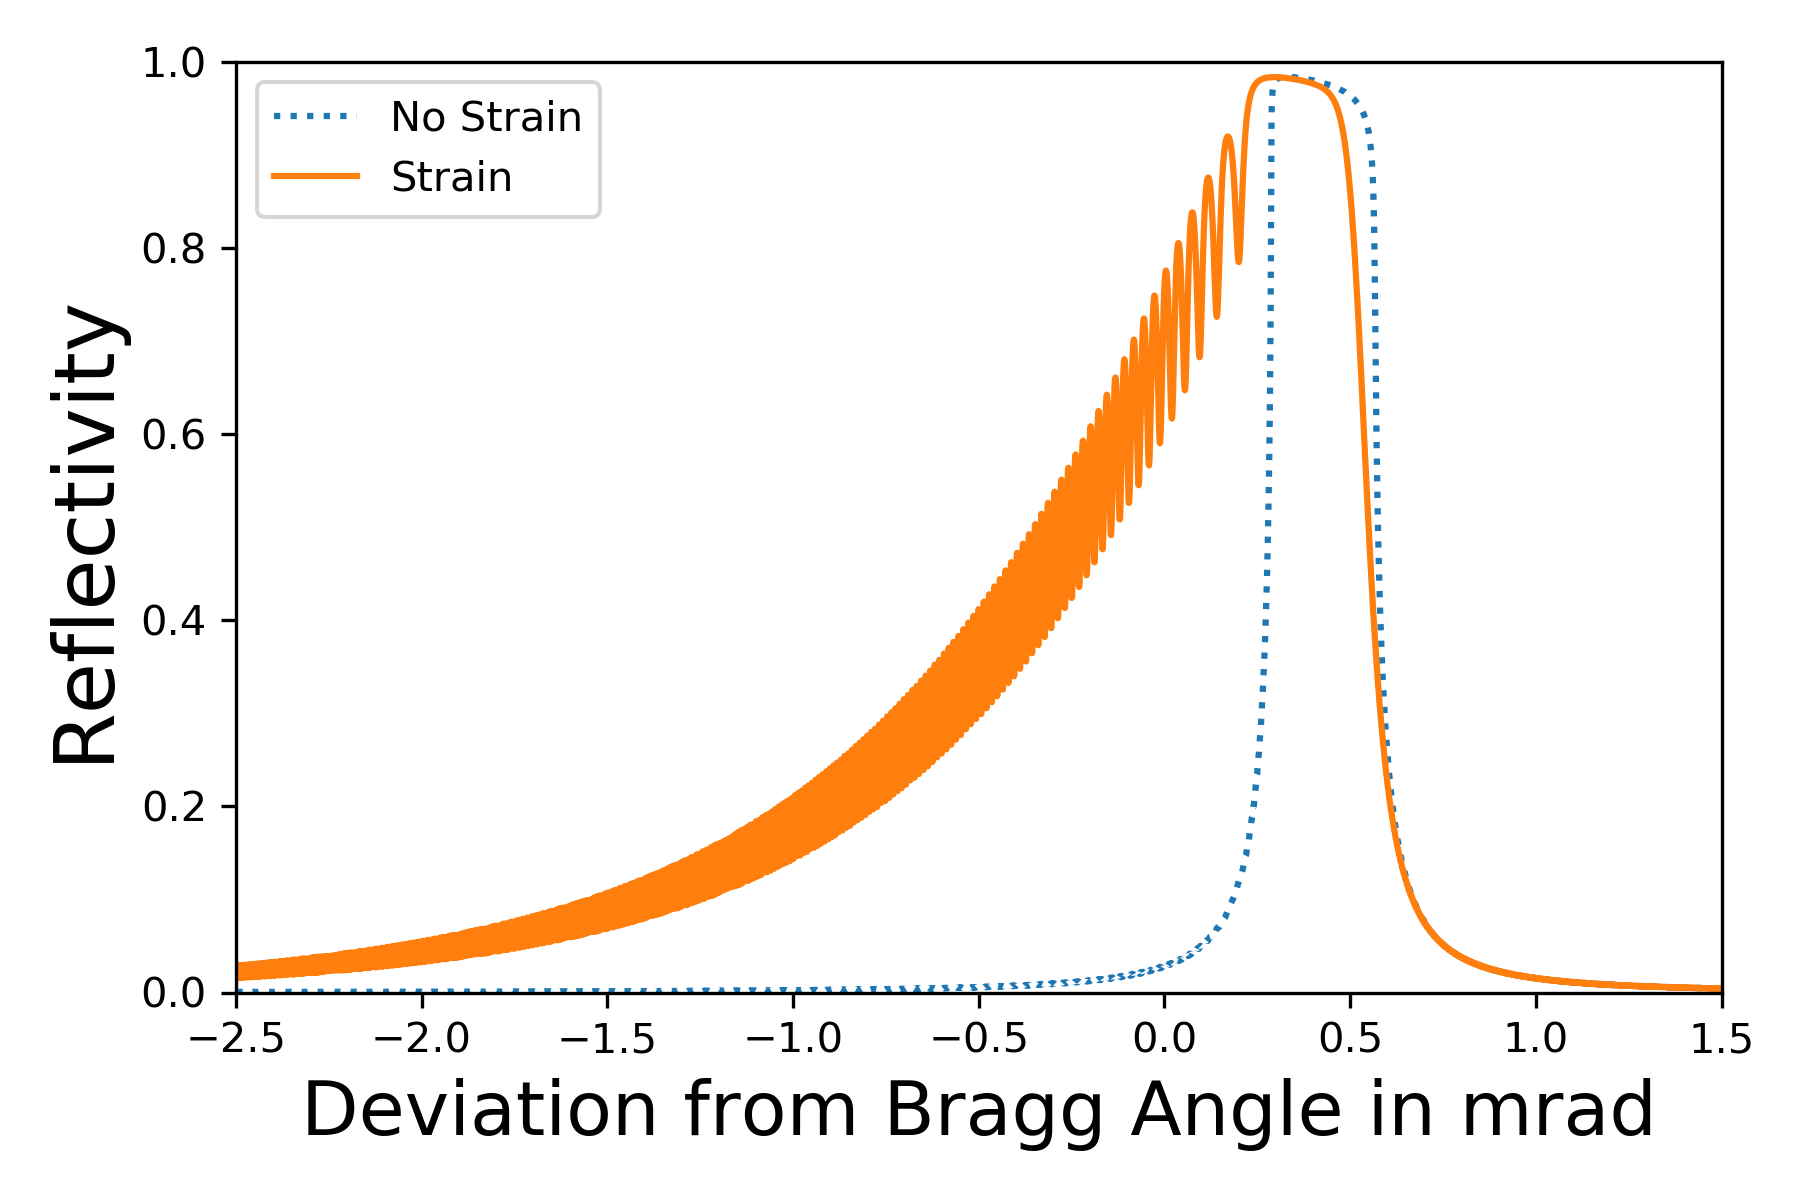
\includegraphics{images/333_20keV_8.png}
\label{fig:333usg20kev}
\end{figure}

\begin{figure}
\caption{HI}
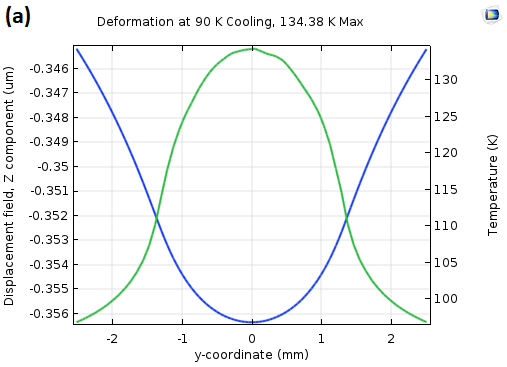
\includegraphics{images/90.png}
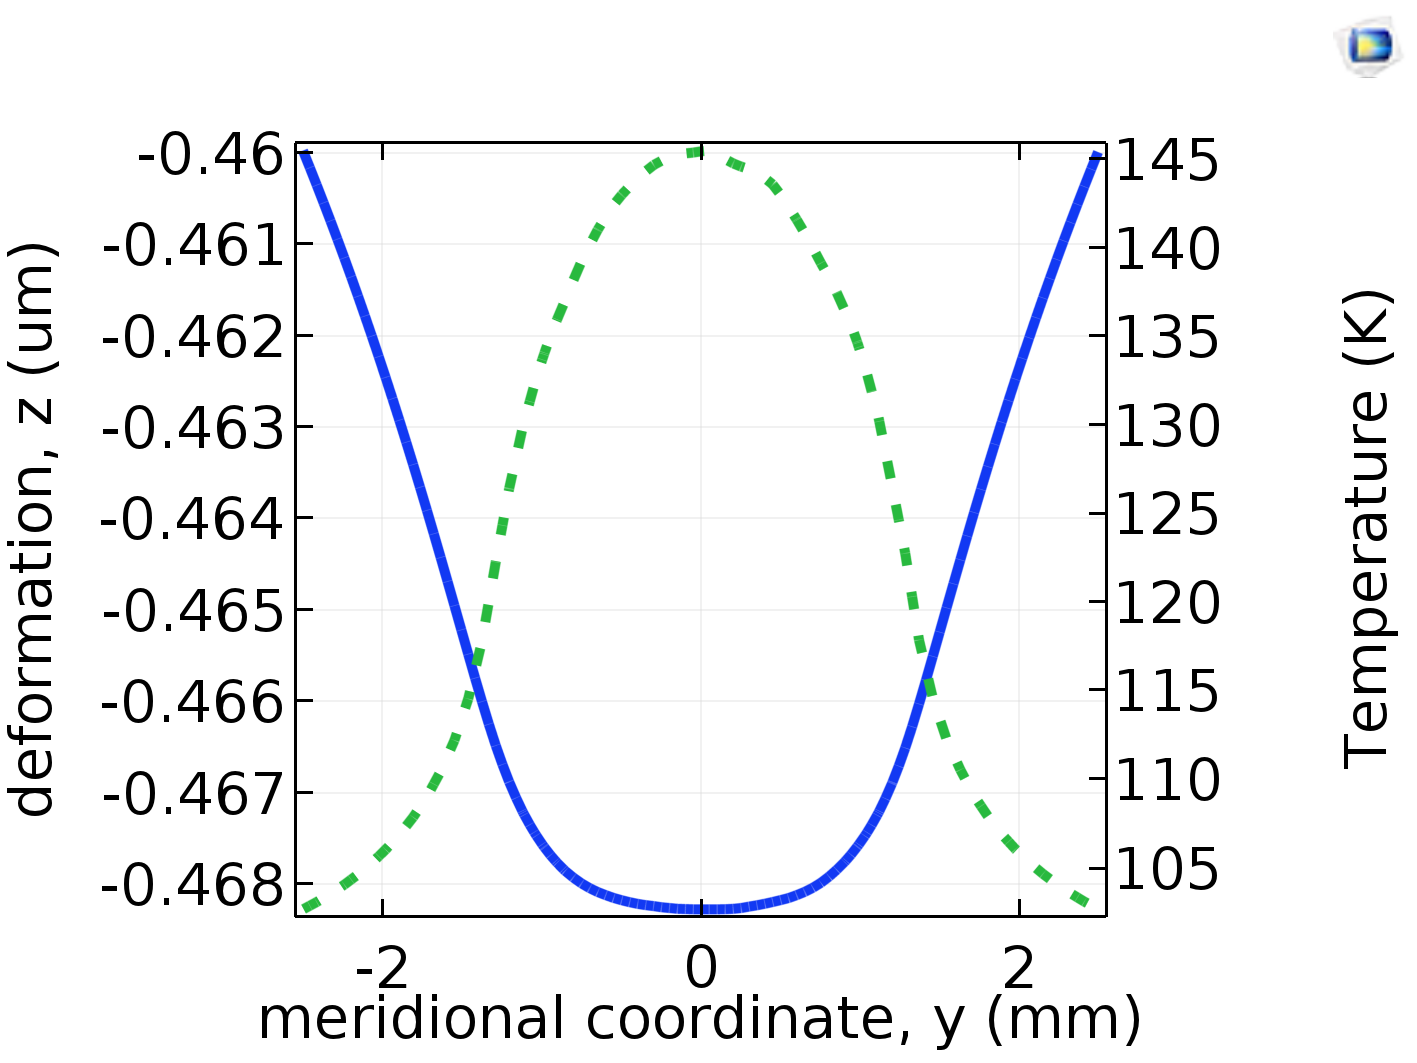
\includegraphics{images/95.png}
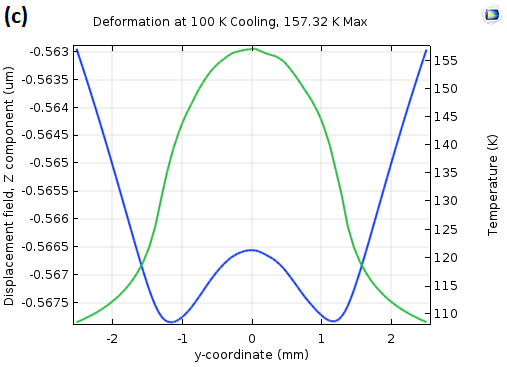
\includegraphics{images/100.png}
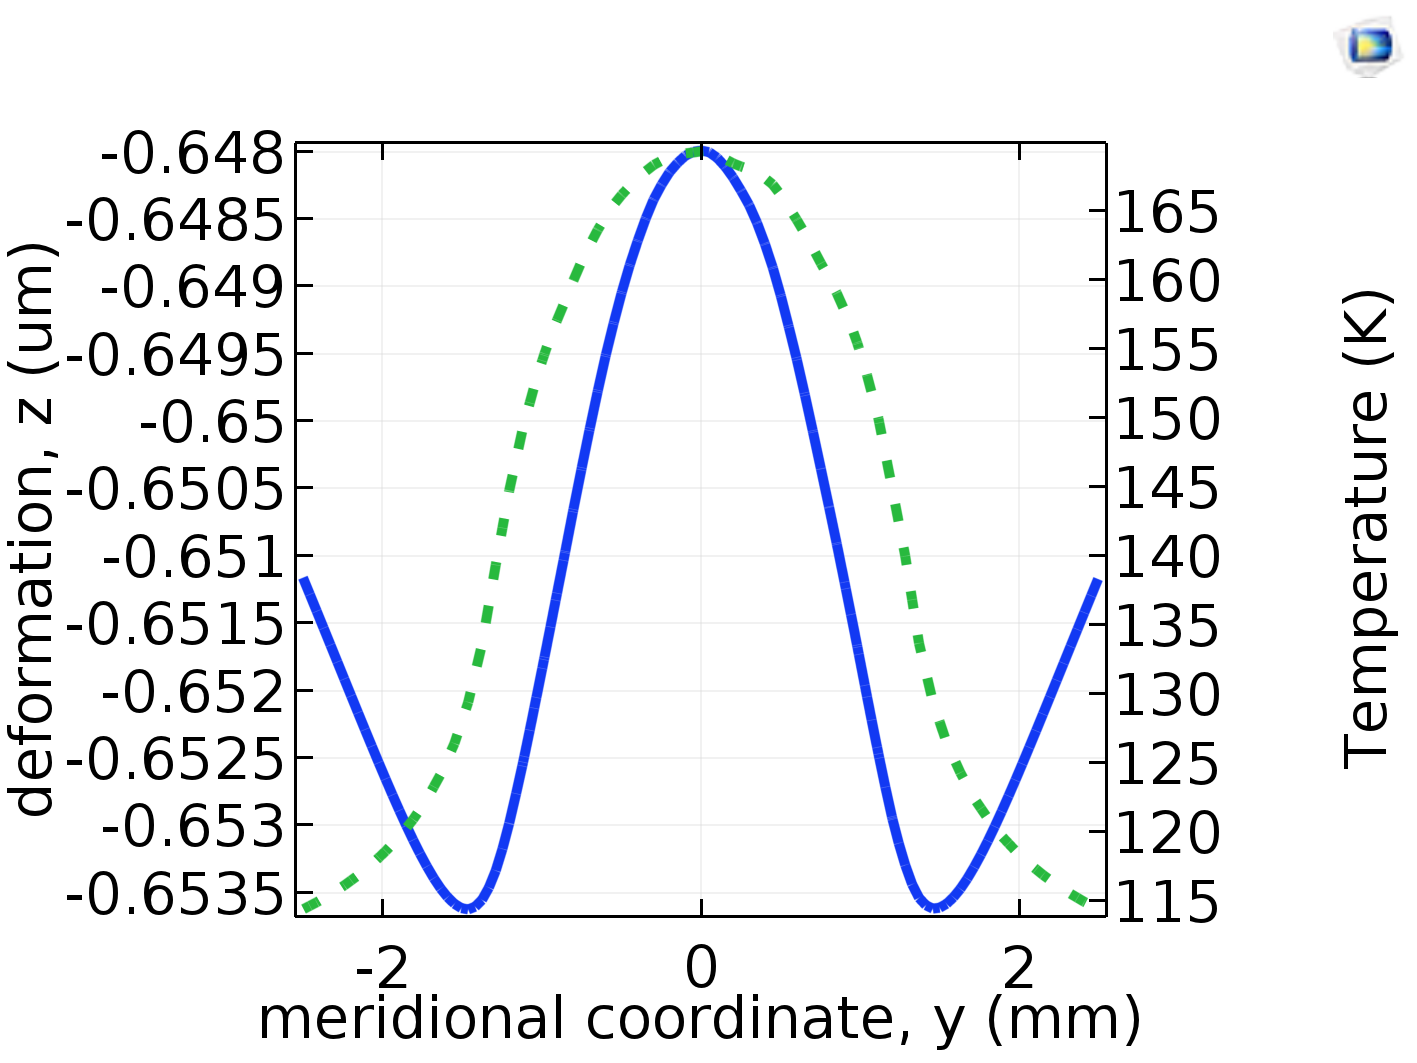
\includegraphics{images/105.png}
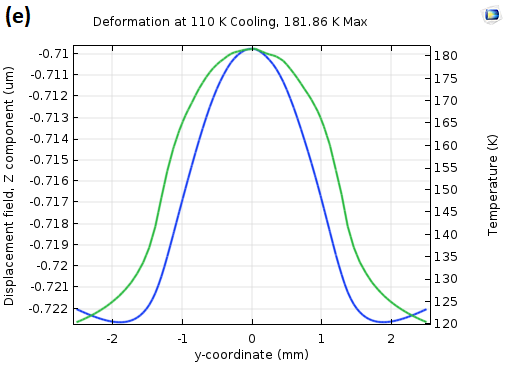
\includegraphics{images/110.png}
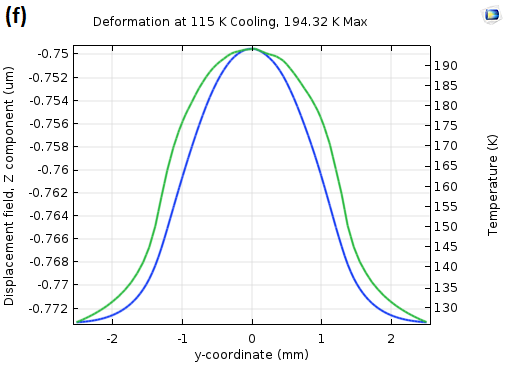
\includegraphics{images/115.png}

\label{fig:ydeformation}
\end{figure}

\begin{figure}
\caption{HI}
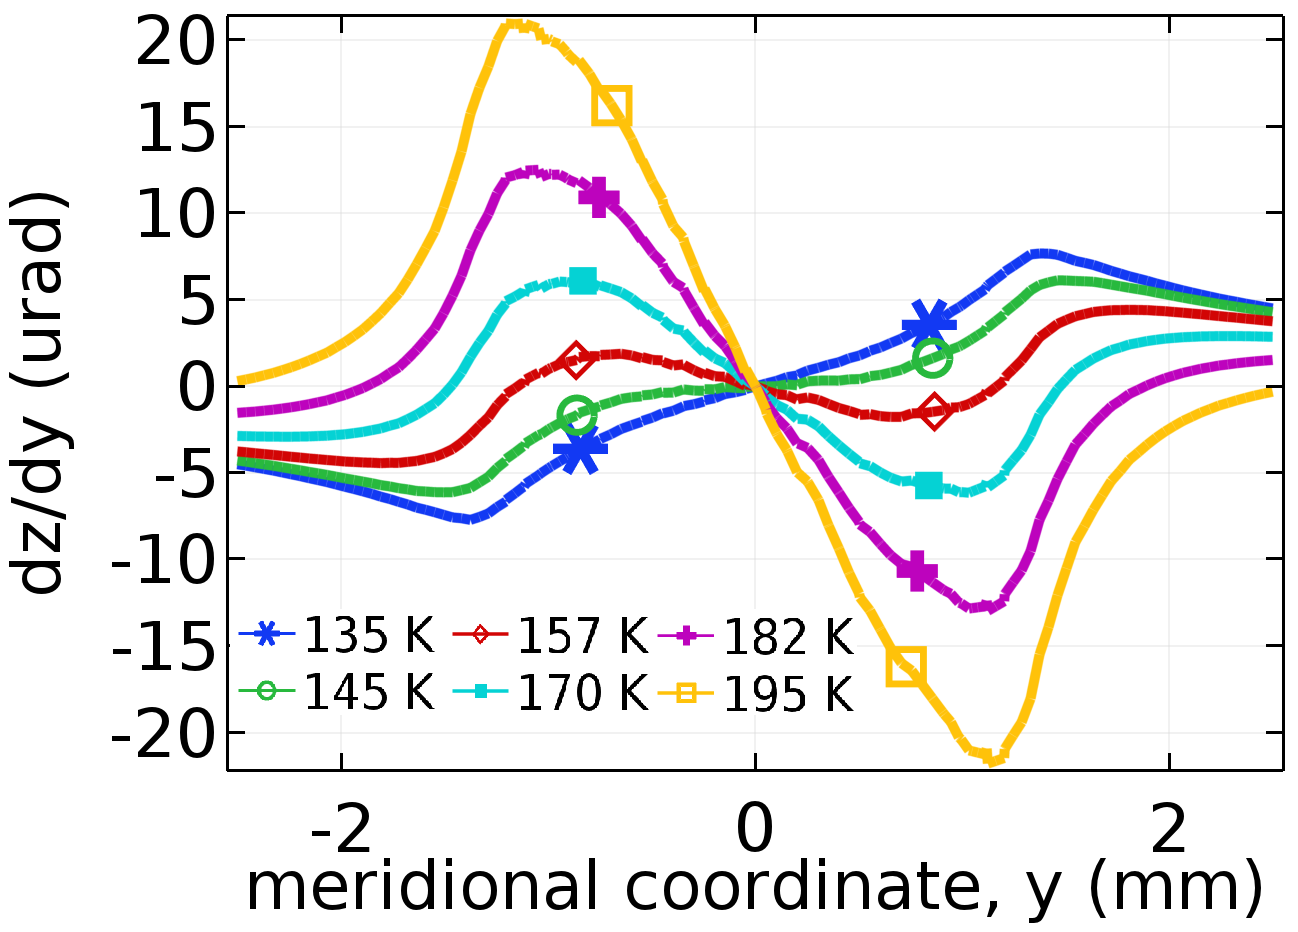
\includegraphics{images/slope.png}
\label{fig:yslope}
\end{figure}

\begin{figure}
\caption{HI}
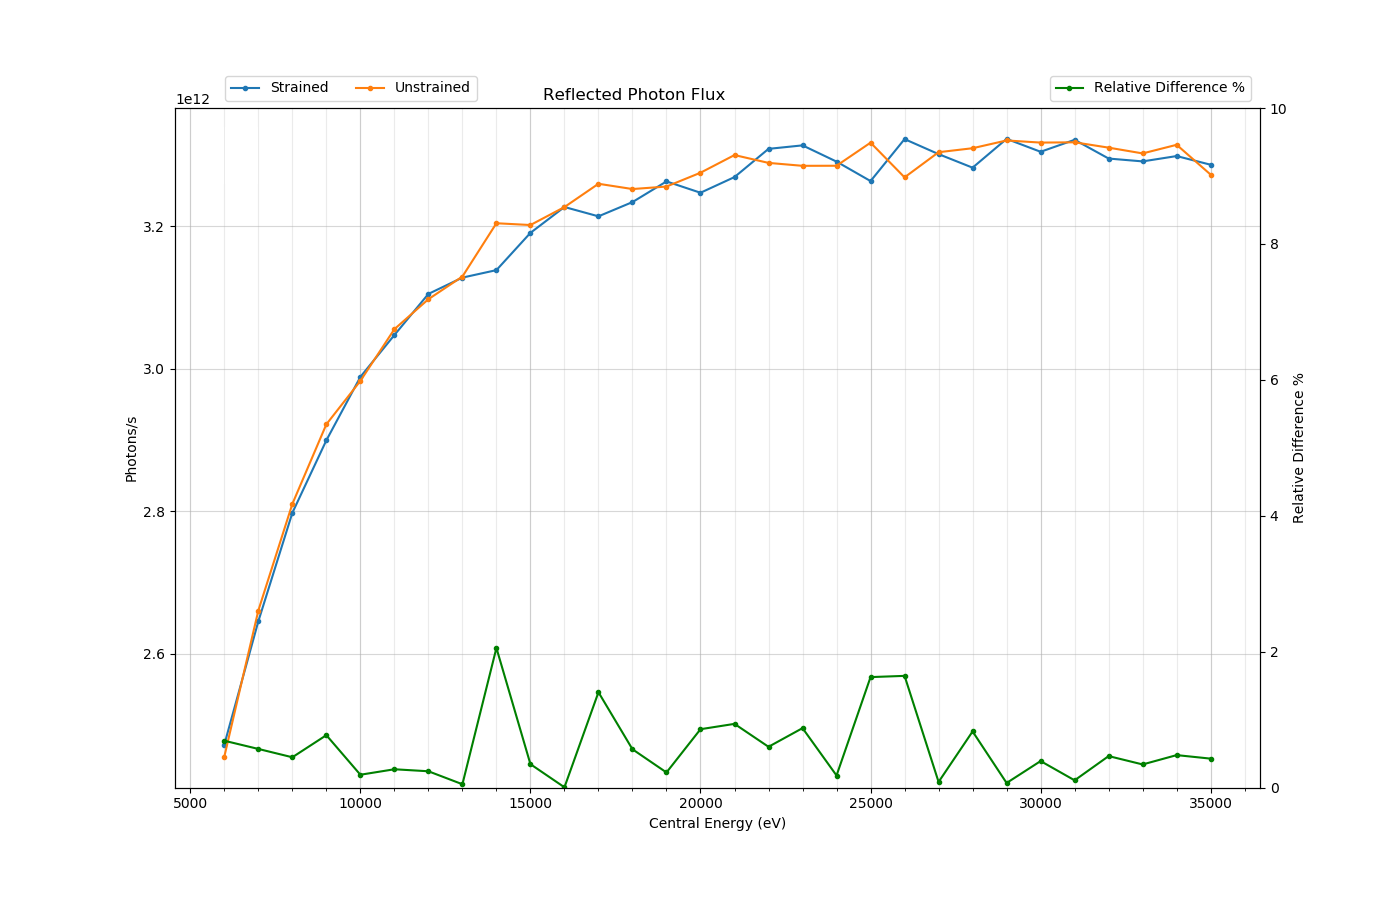
\includegraphics{images/111flux.png}
\label{fig:111flux}
\end{figure}

\begin{figure}
\caption{HI}
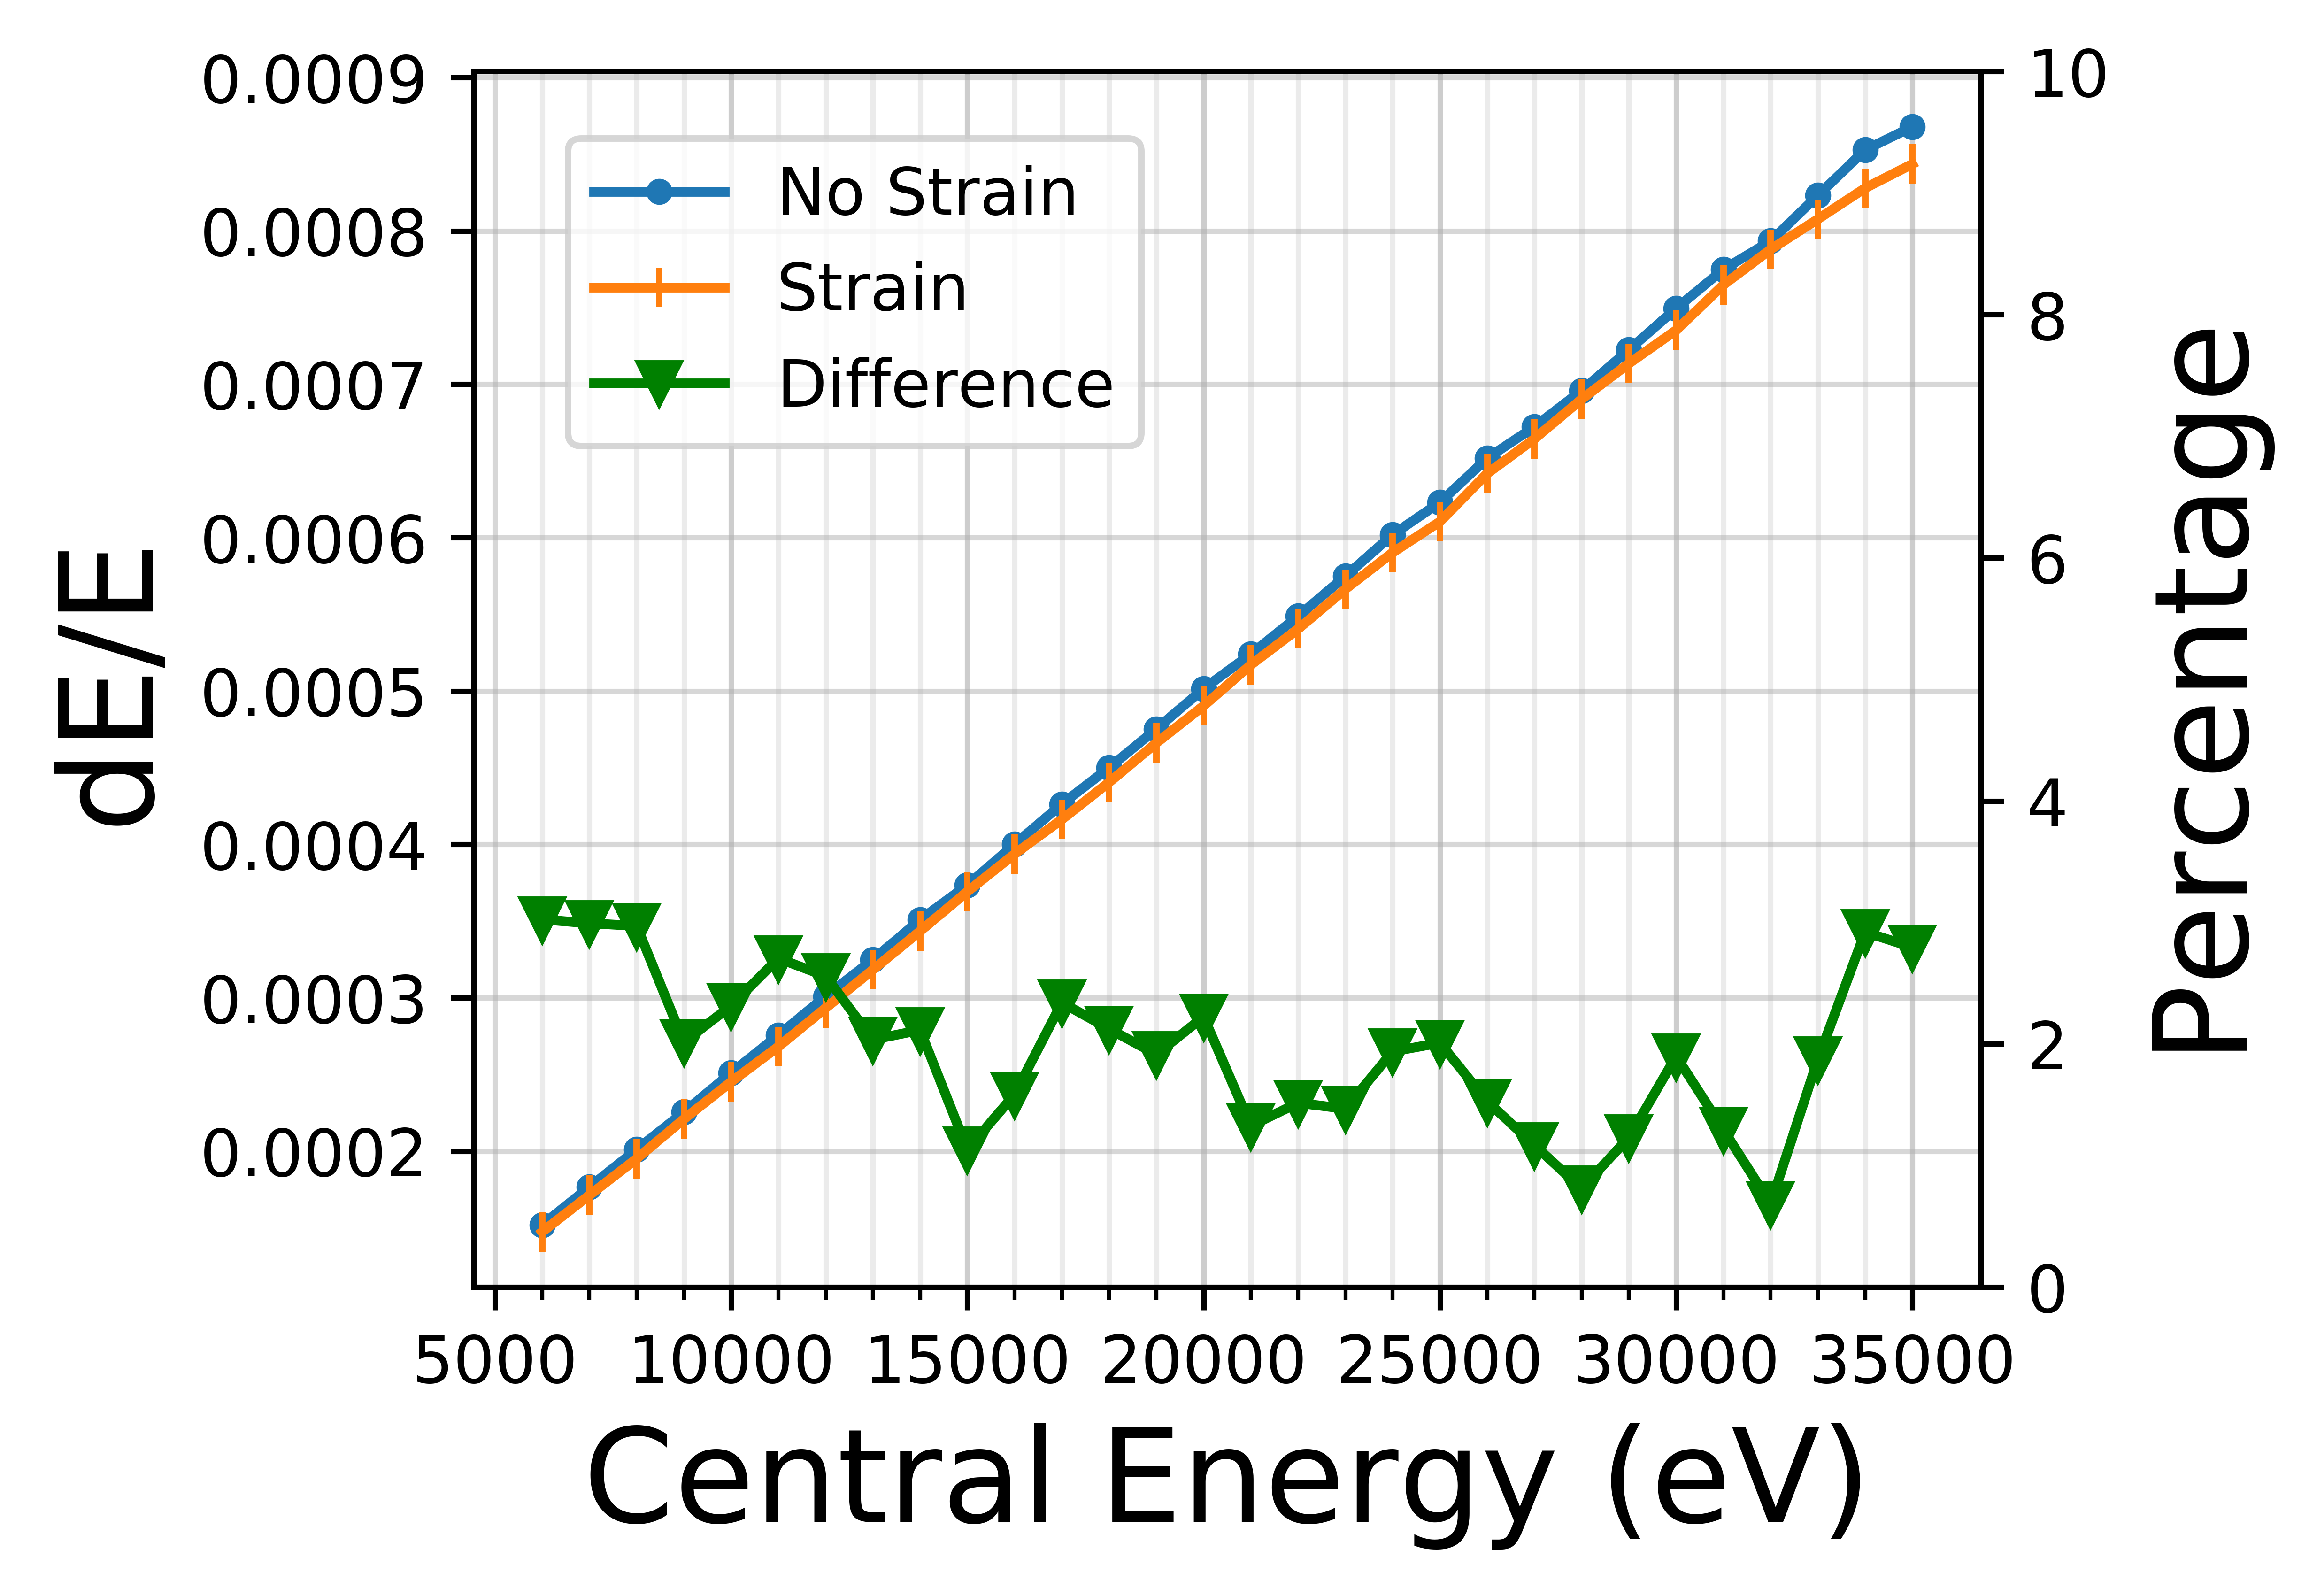
\includegraphics{images/111monobw.png}
\label{fig:111monobw}
\end{figure}

\begin{figure}
\caption{HI}
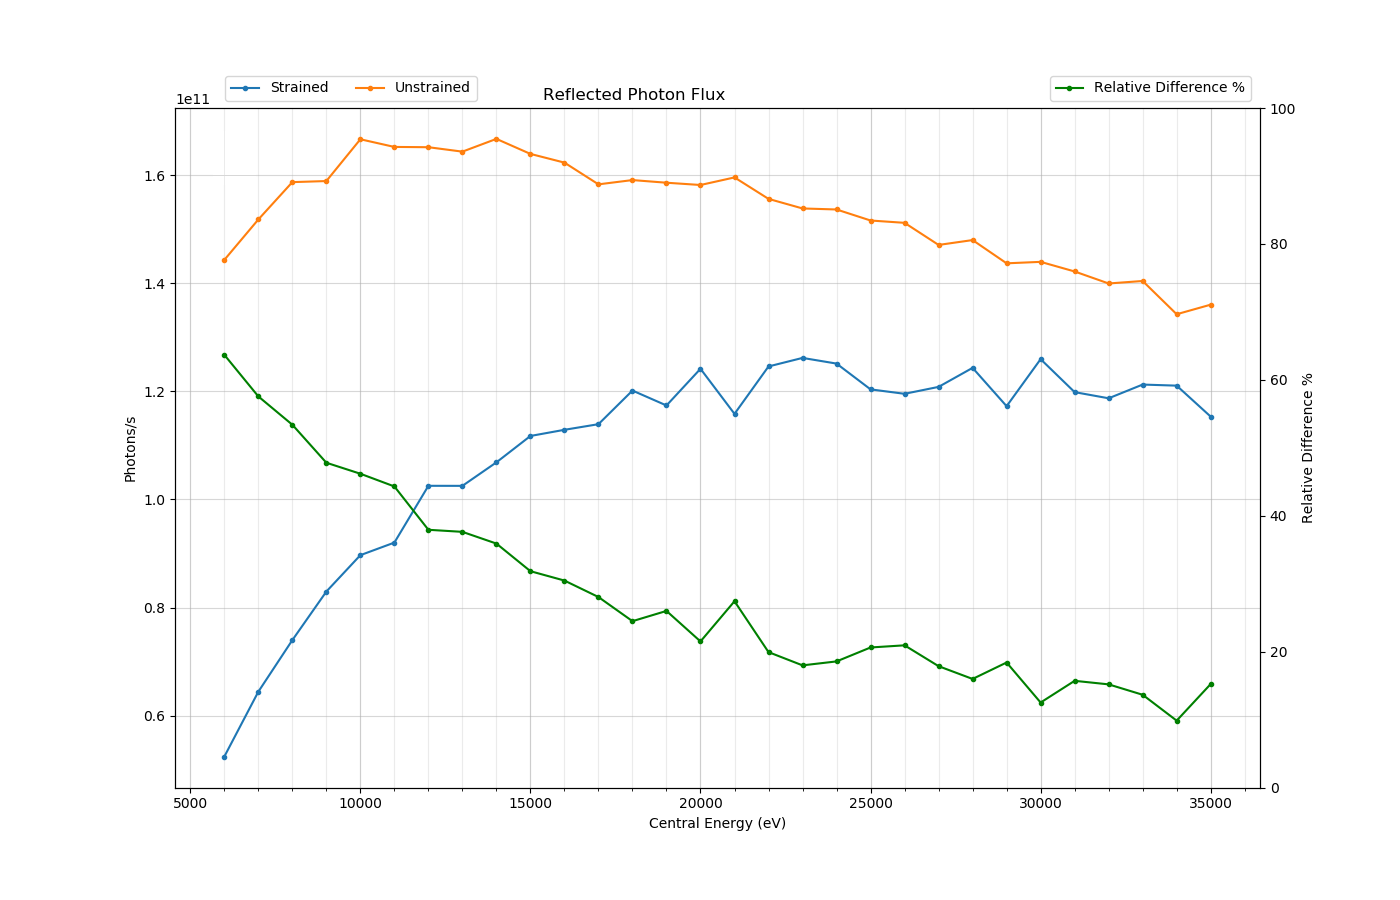
\includegraphics{images/333flux.png}
\label{fig:333flux}
\end{figure}

\begin{figure}
\caption{HI}
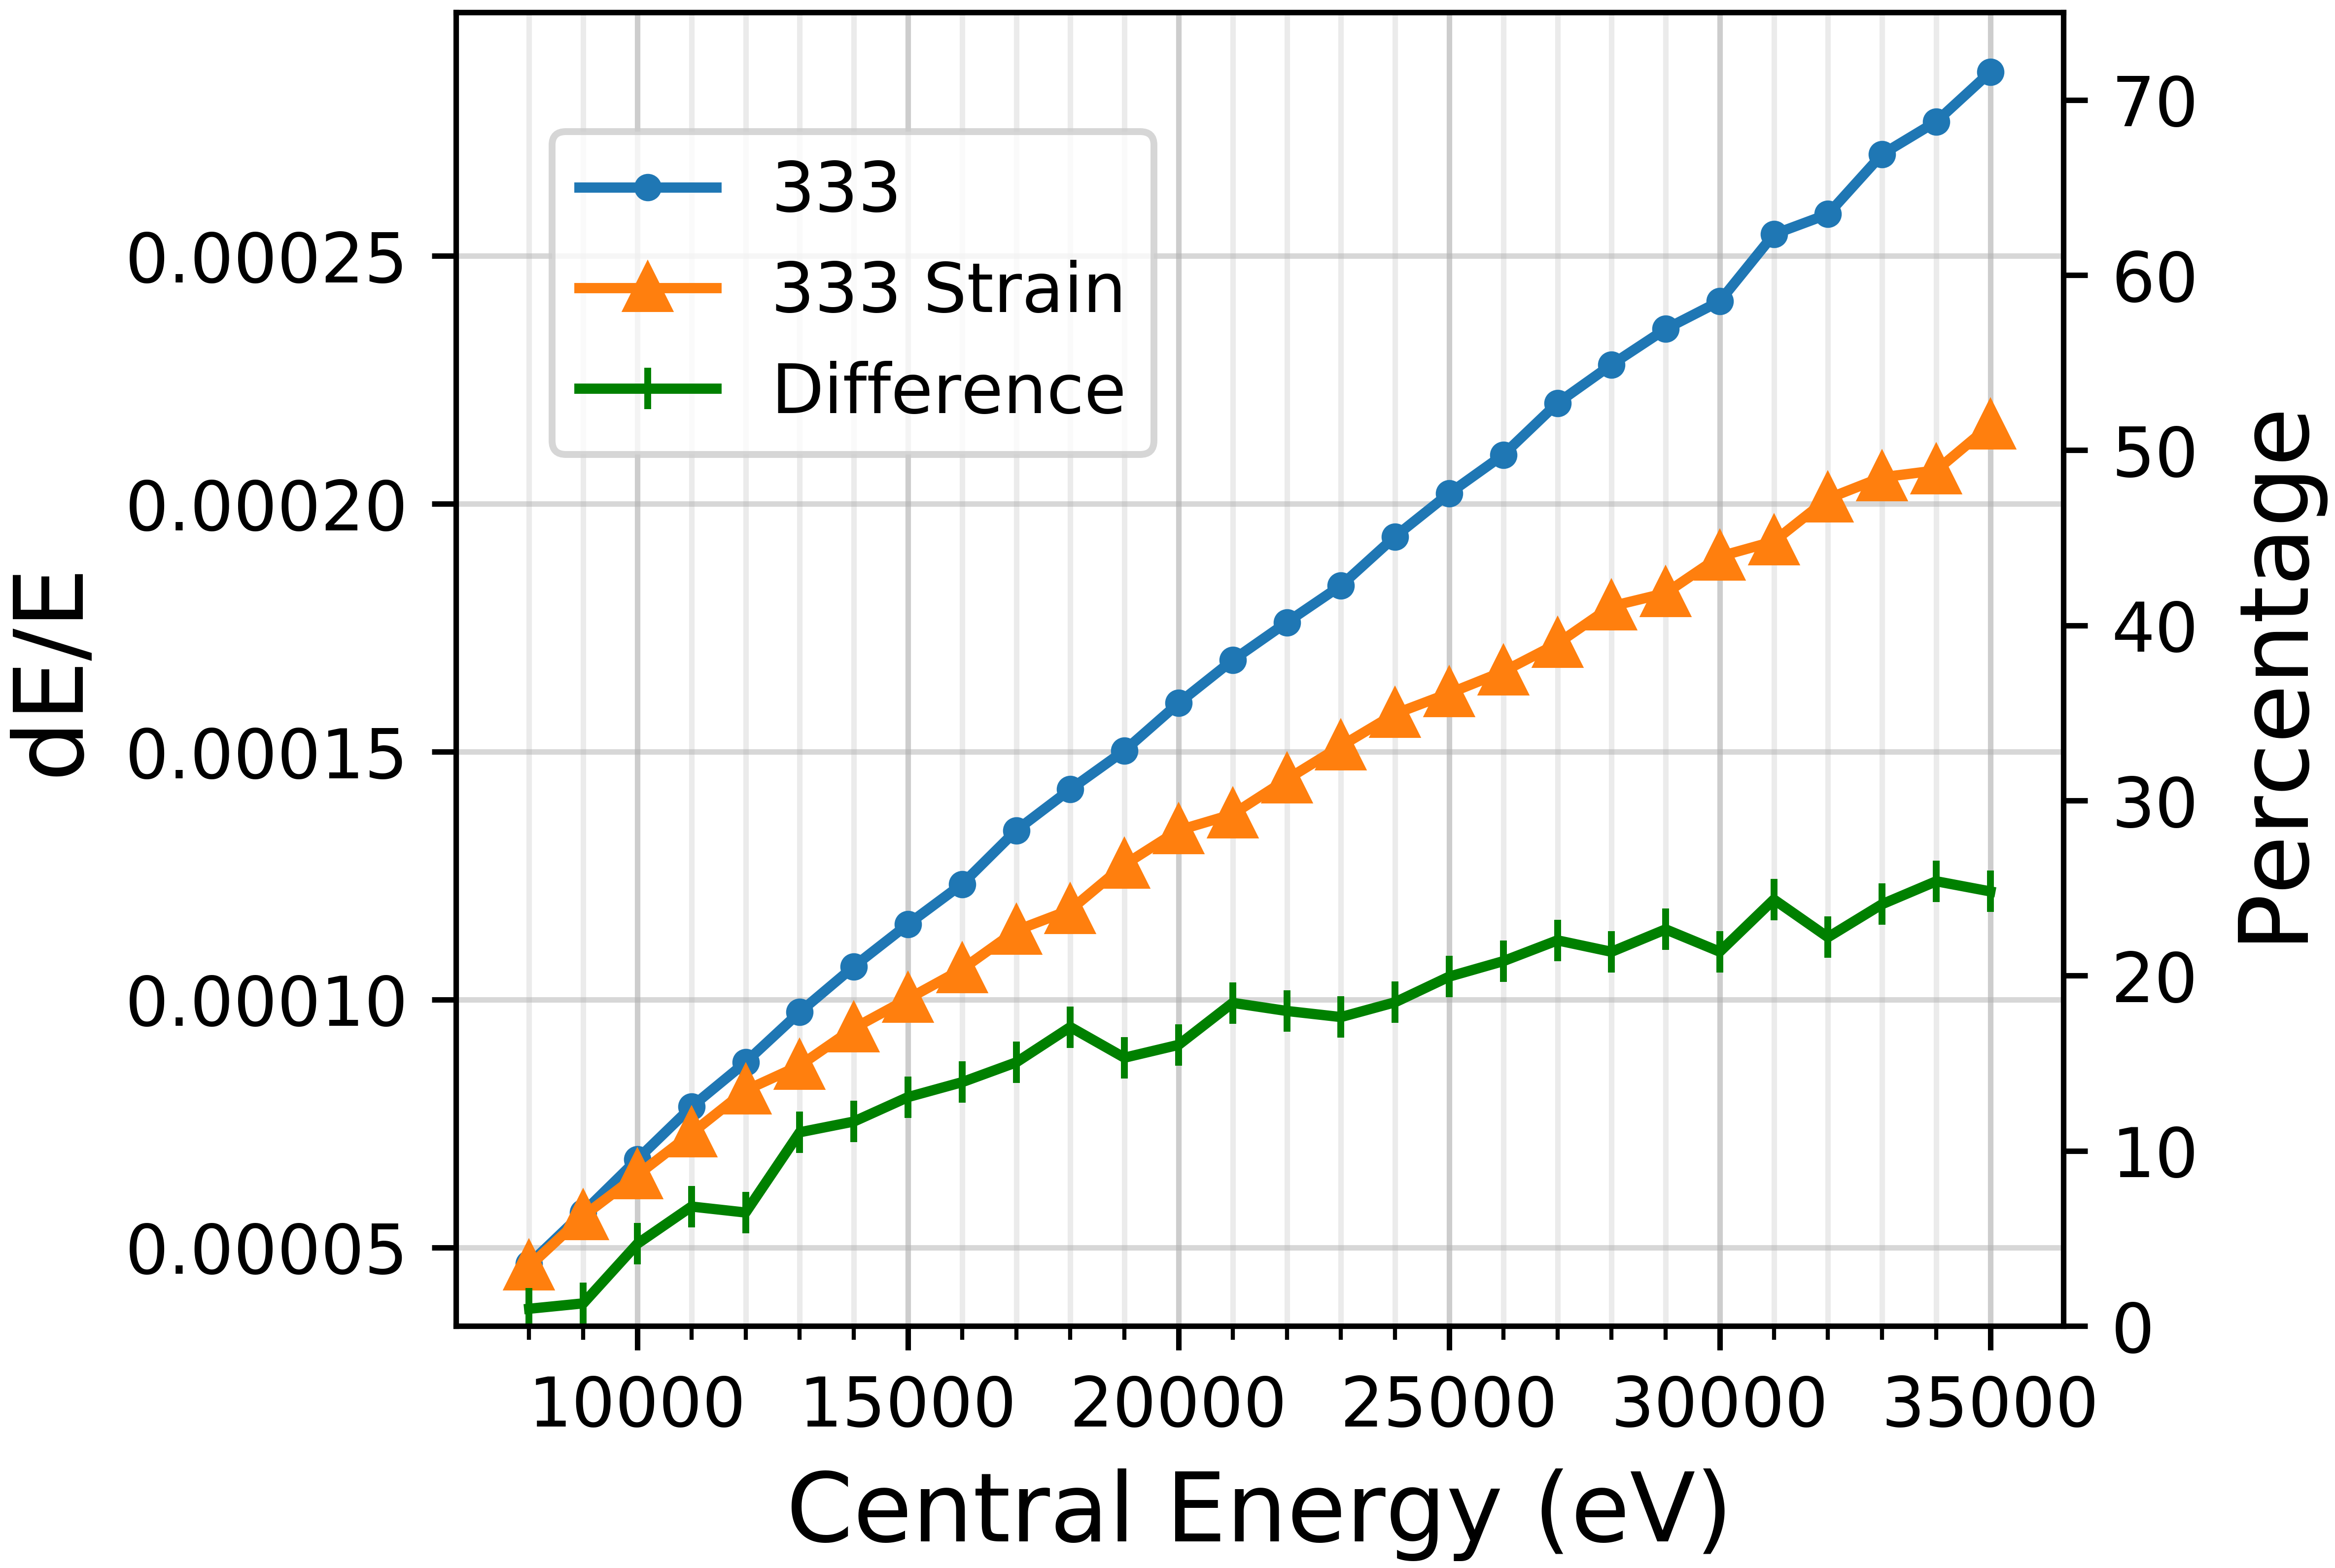
\includegraphics{images/333monobw.png}
\label{fig:333monobw}
\end{figure}

\begin{figure}
\caption{in watts}
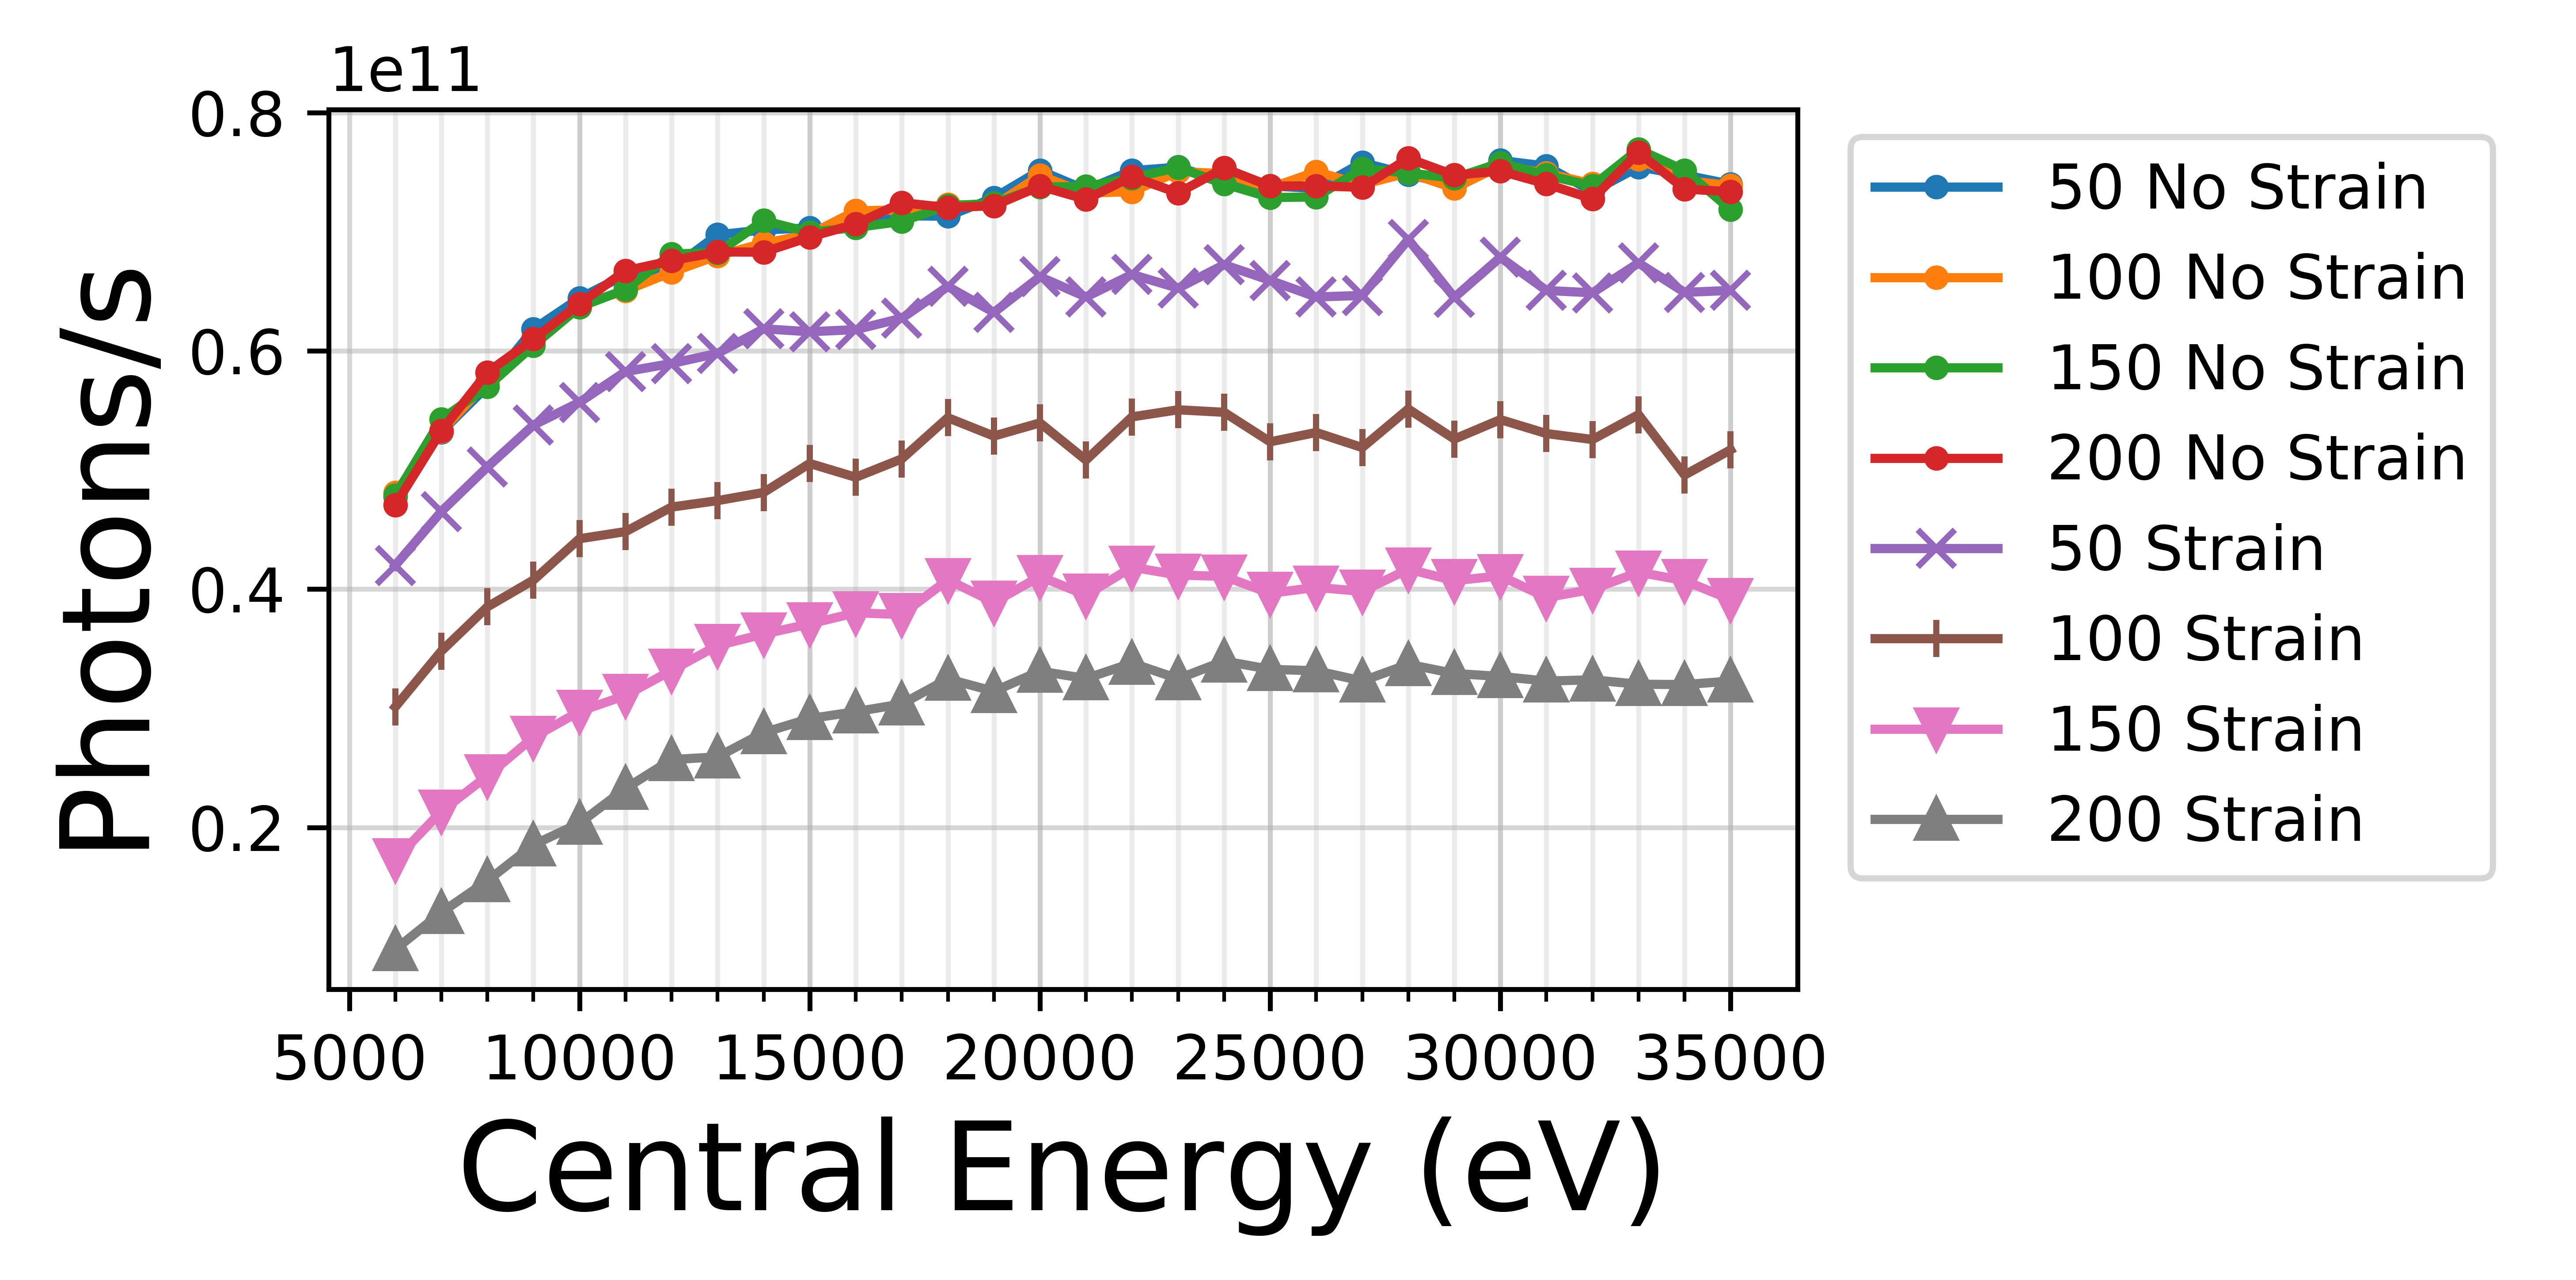
\includegraphics{images/333strainpower.png}
\label{fig:333strainpower}
\end{figure}


\begin{figure}
\caption{in meters}
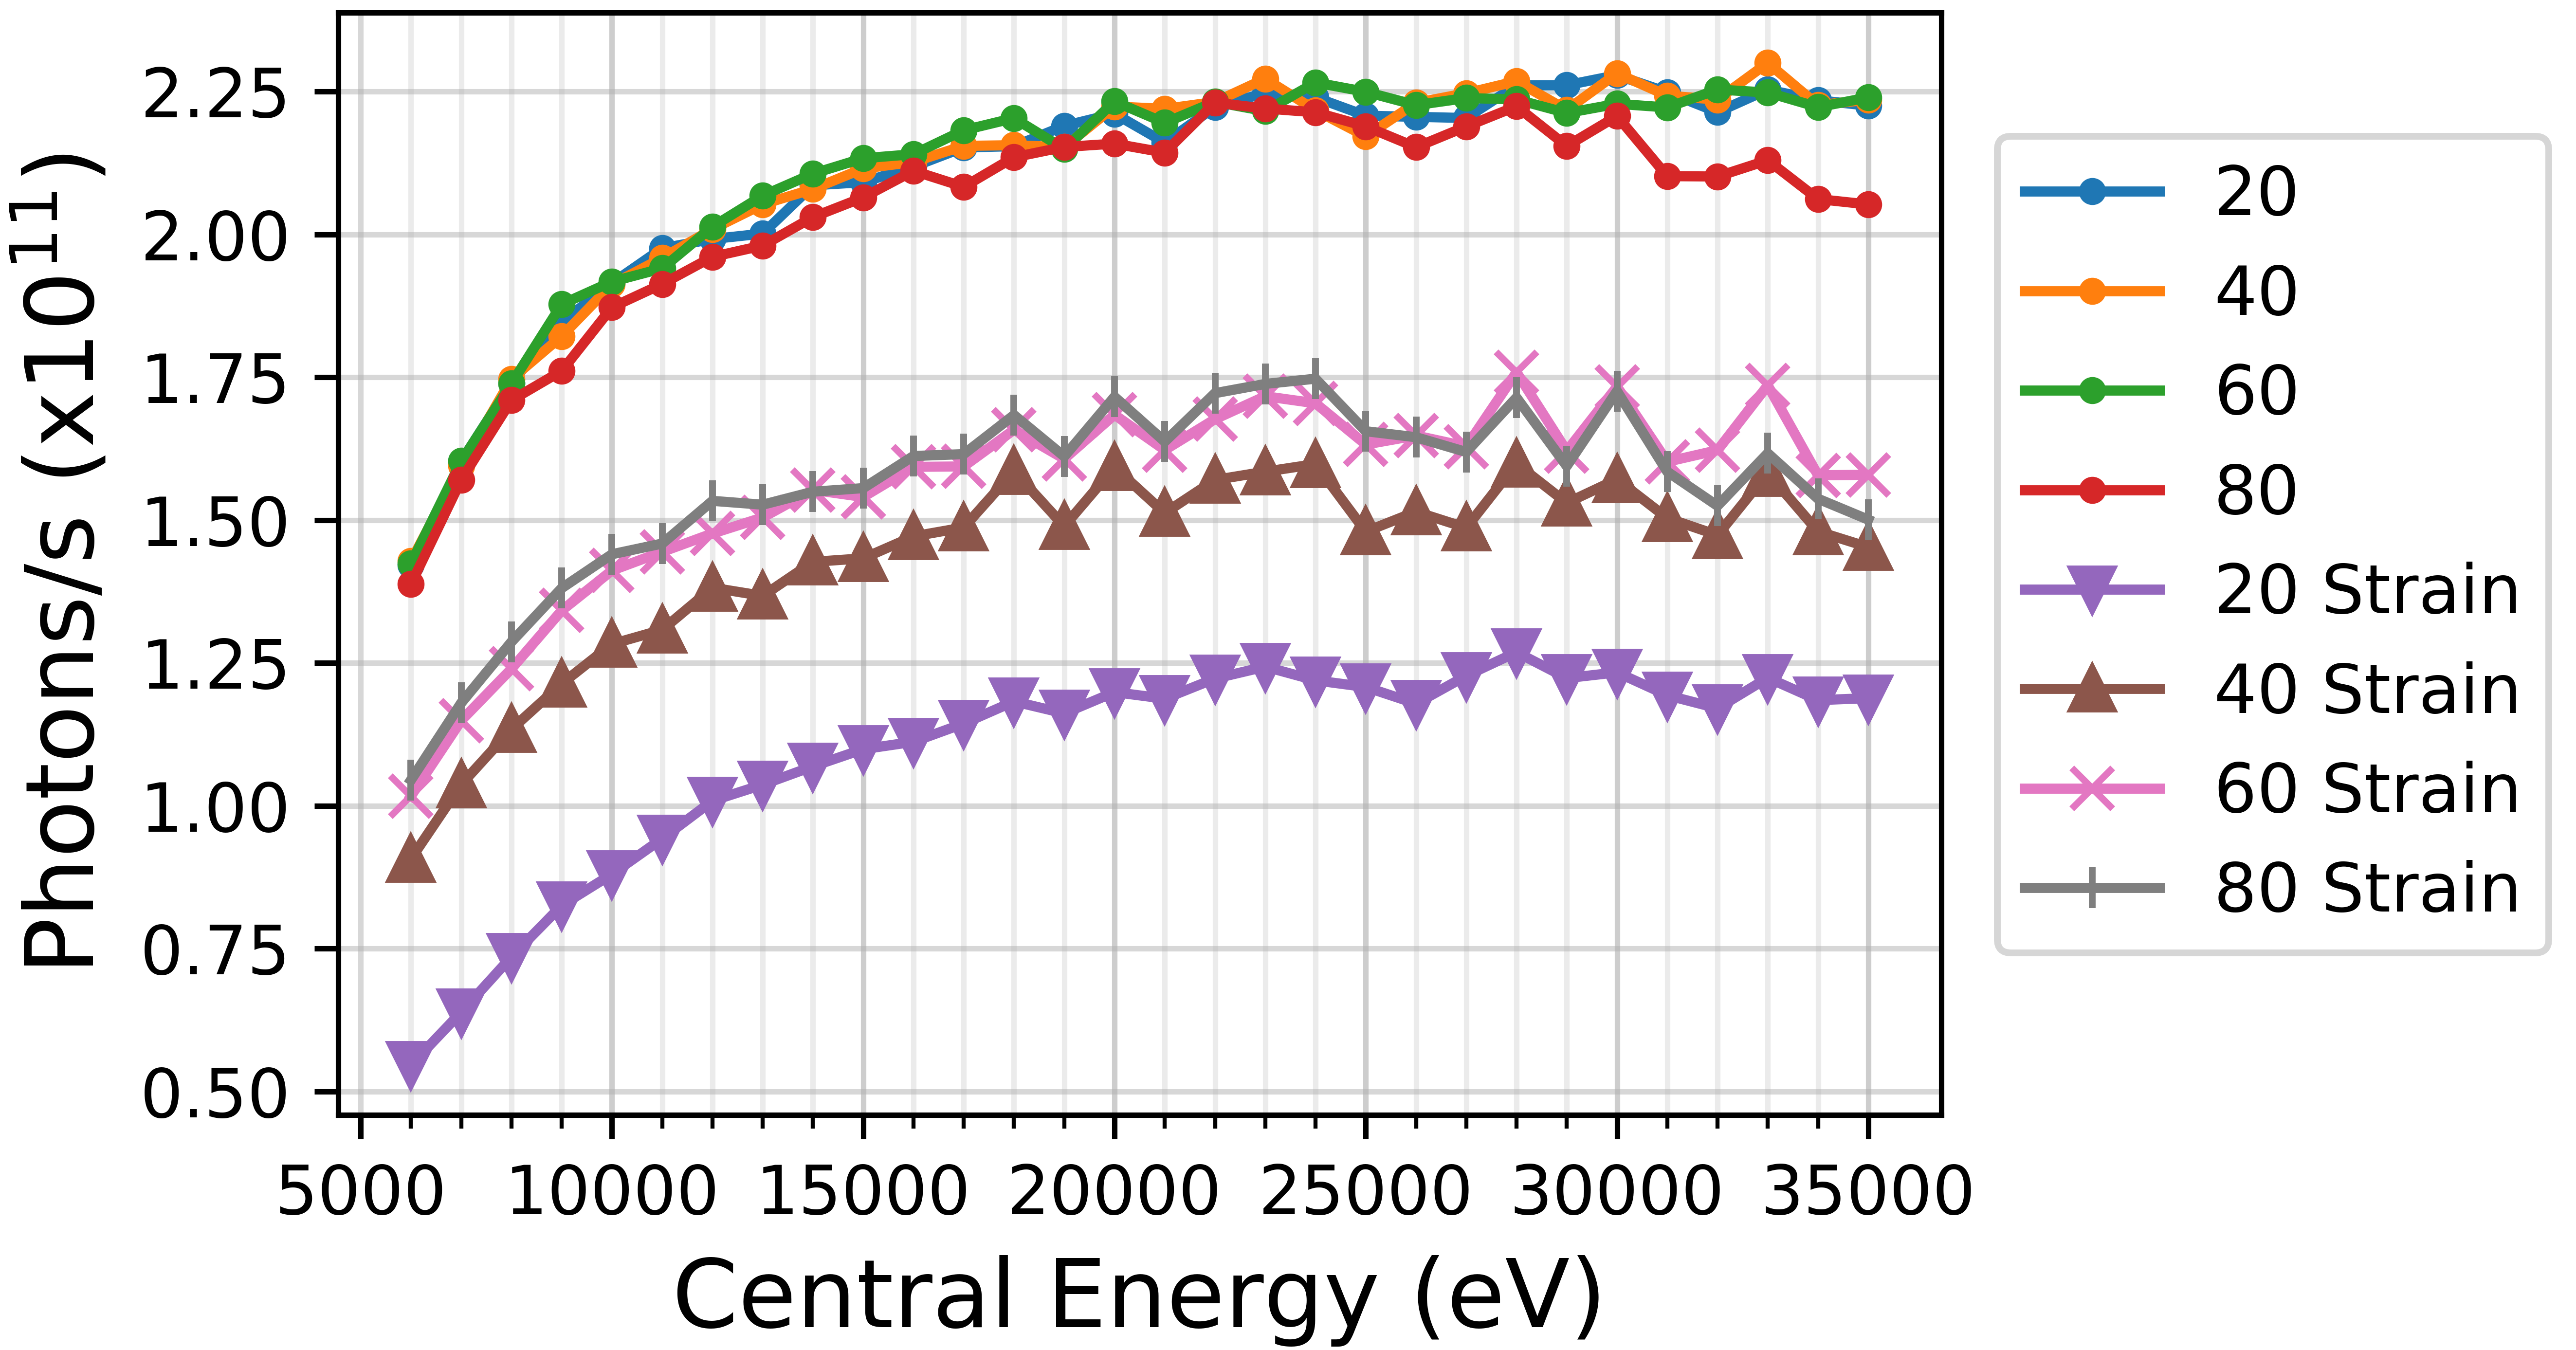
\includegraphics{images/333straindistance.png}
\label{fig:333straindistance}
\end{figure}

\begin{figure}
\caption{in what units?}
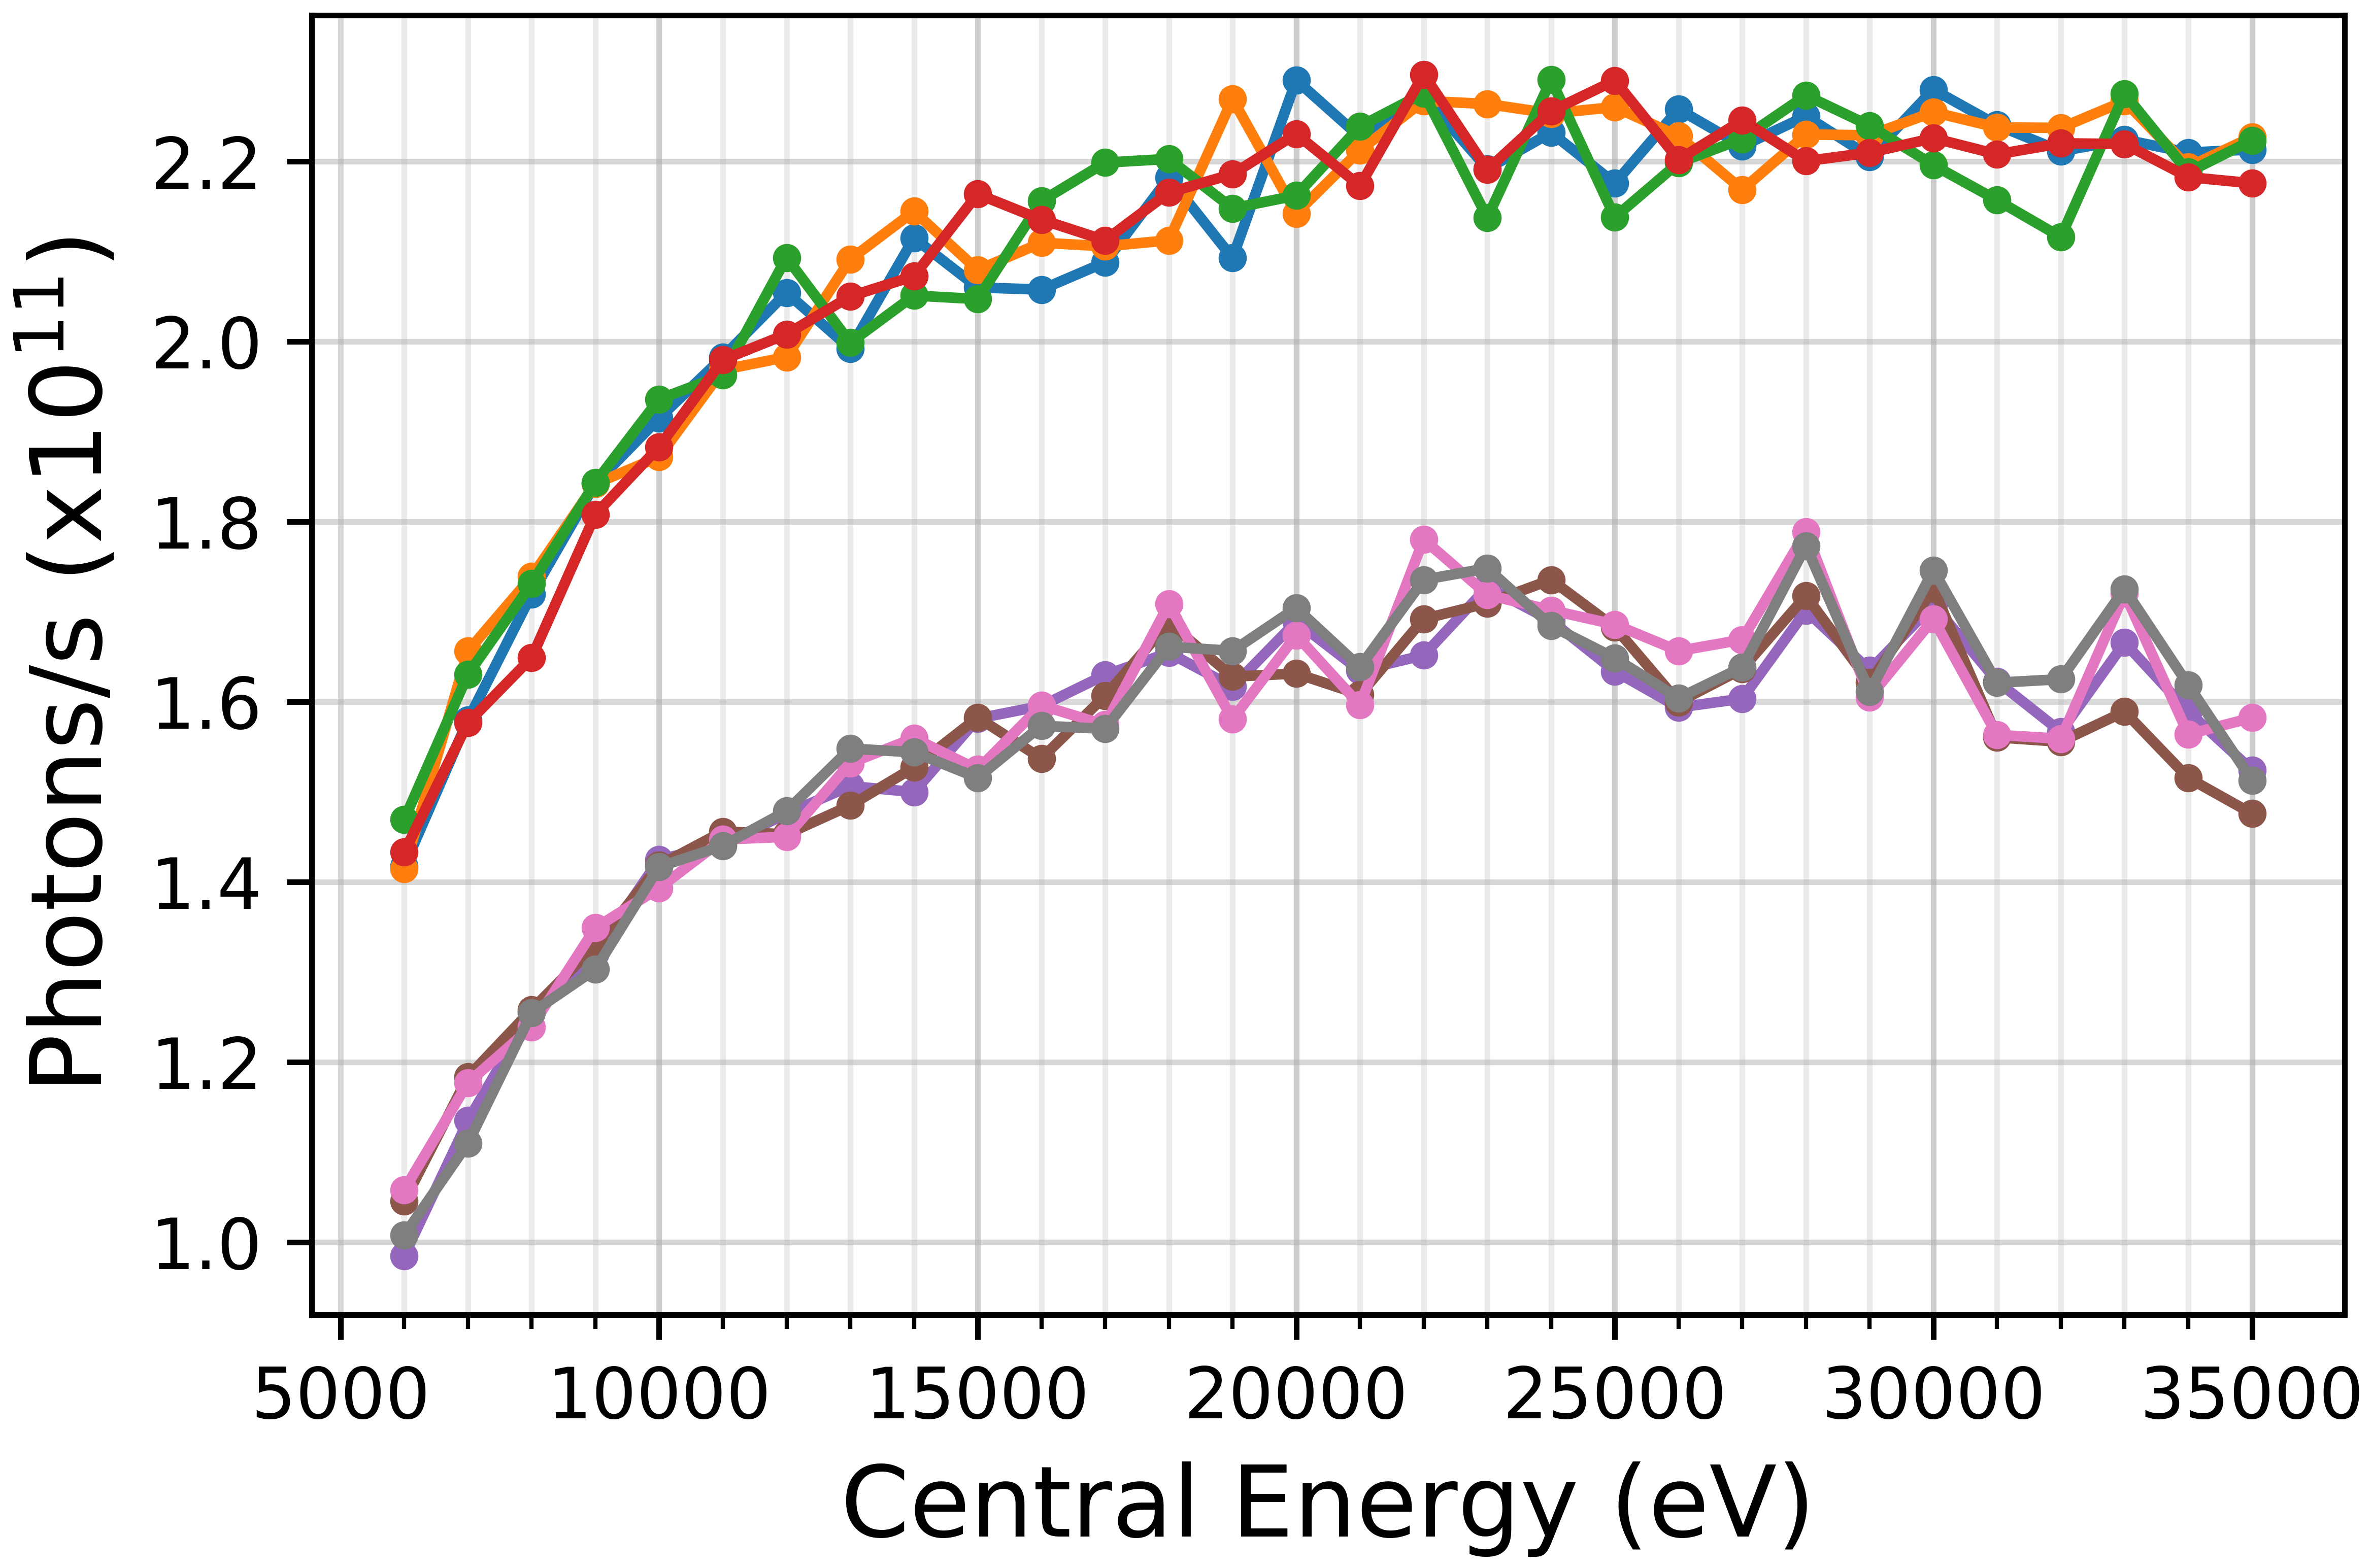
\includegraphics{images/333straindivergence.png}
\label{fig:333straindivergence}
\end{figure}

\begin{figure}
\caption{in what units?}
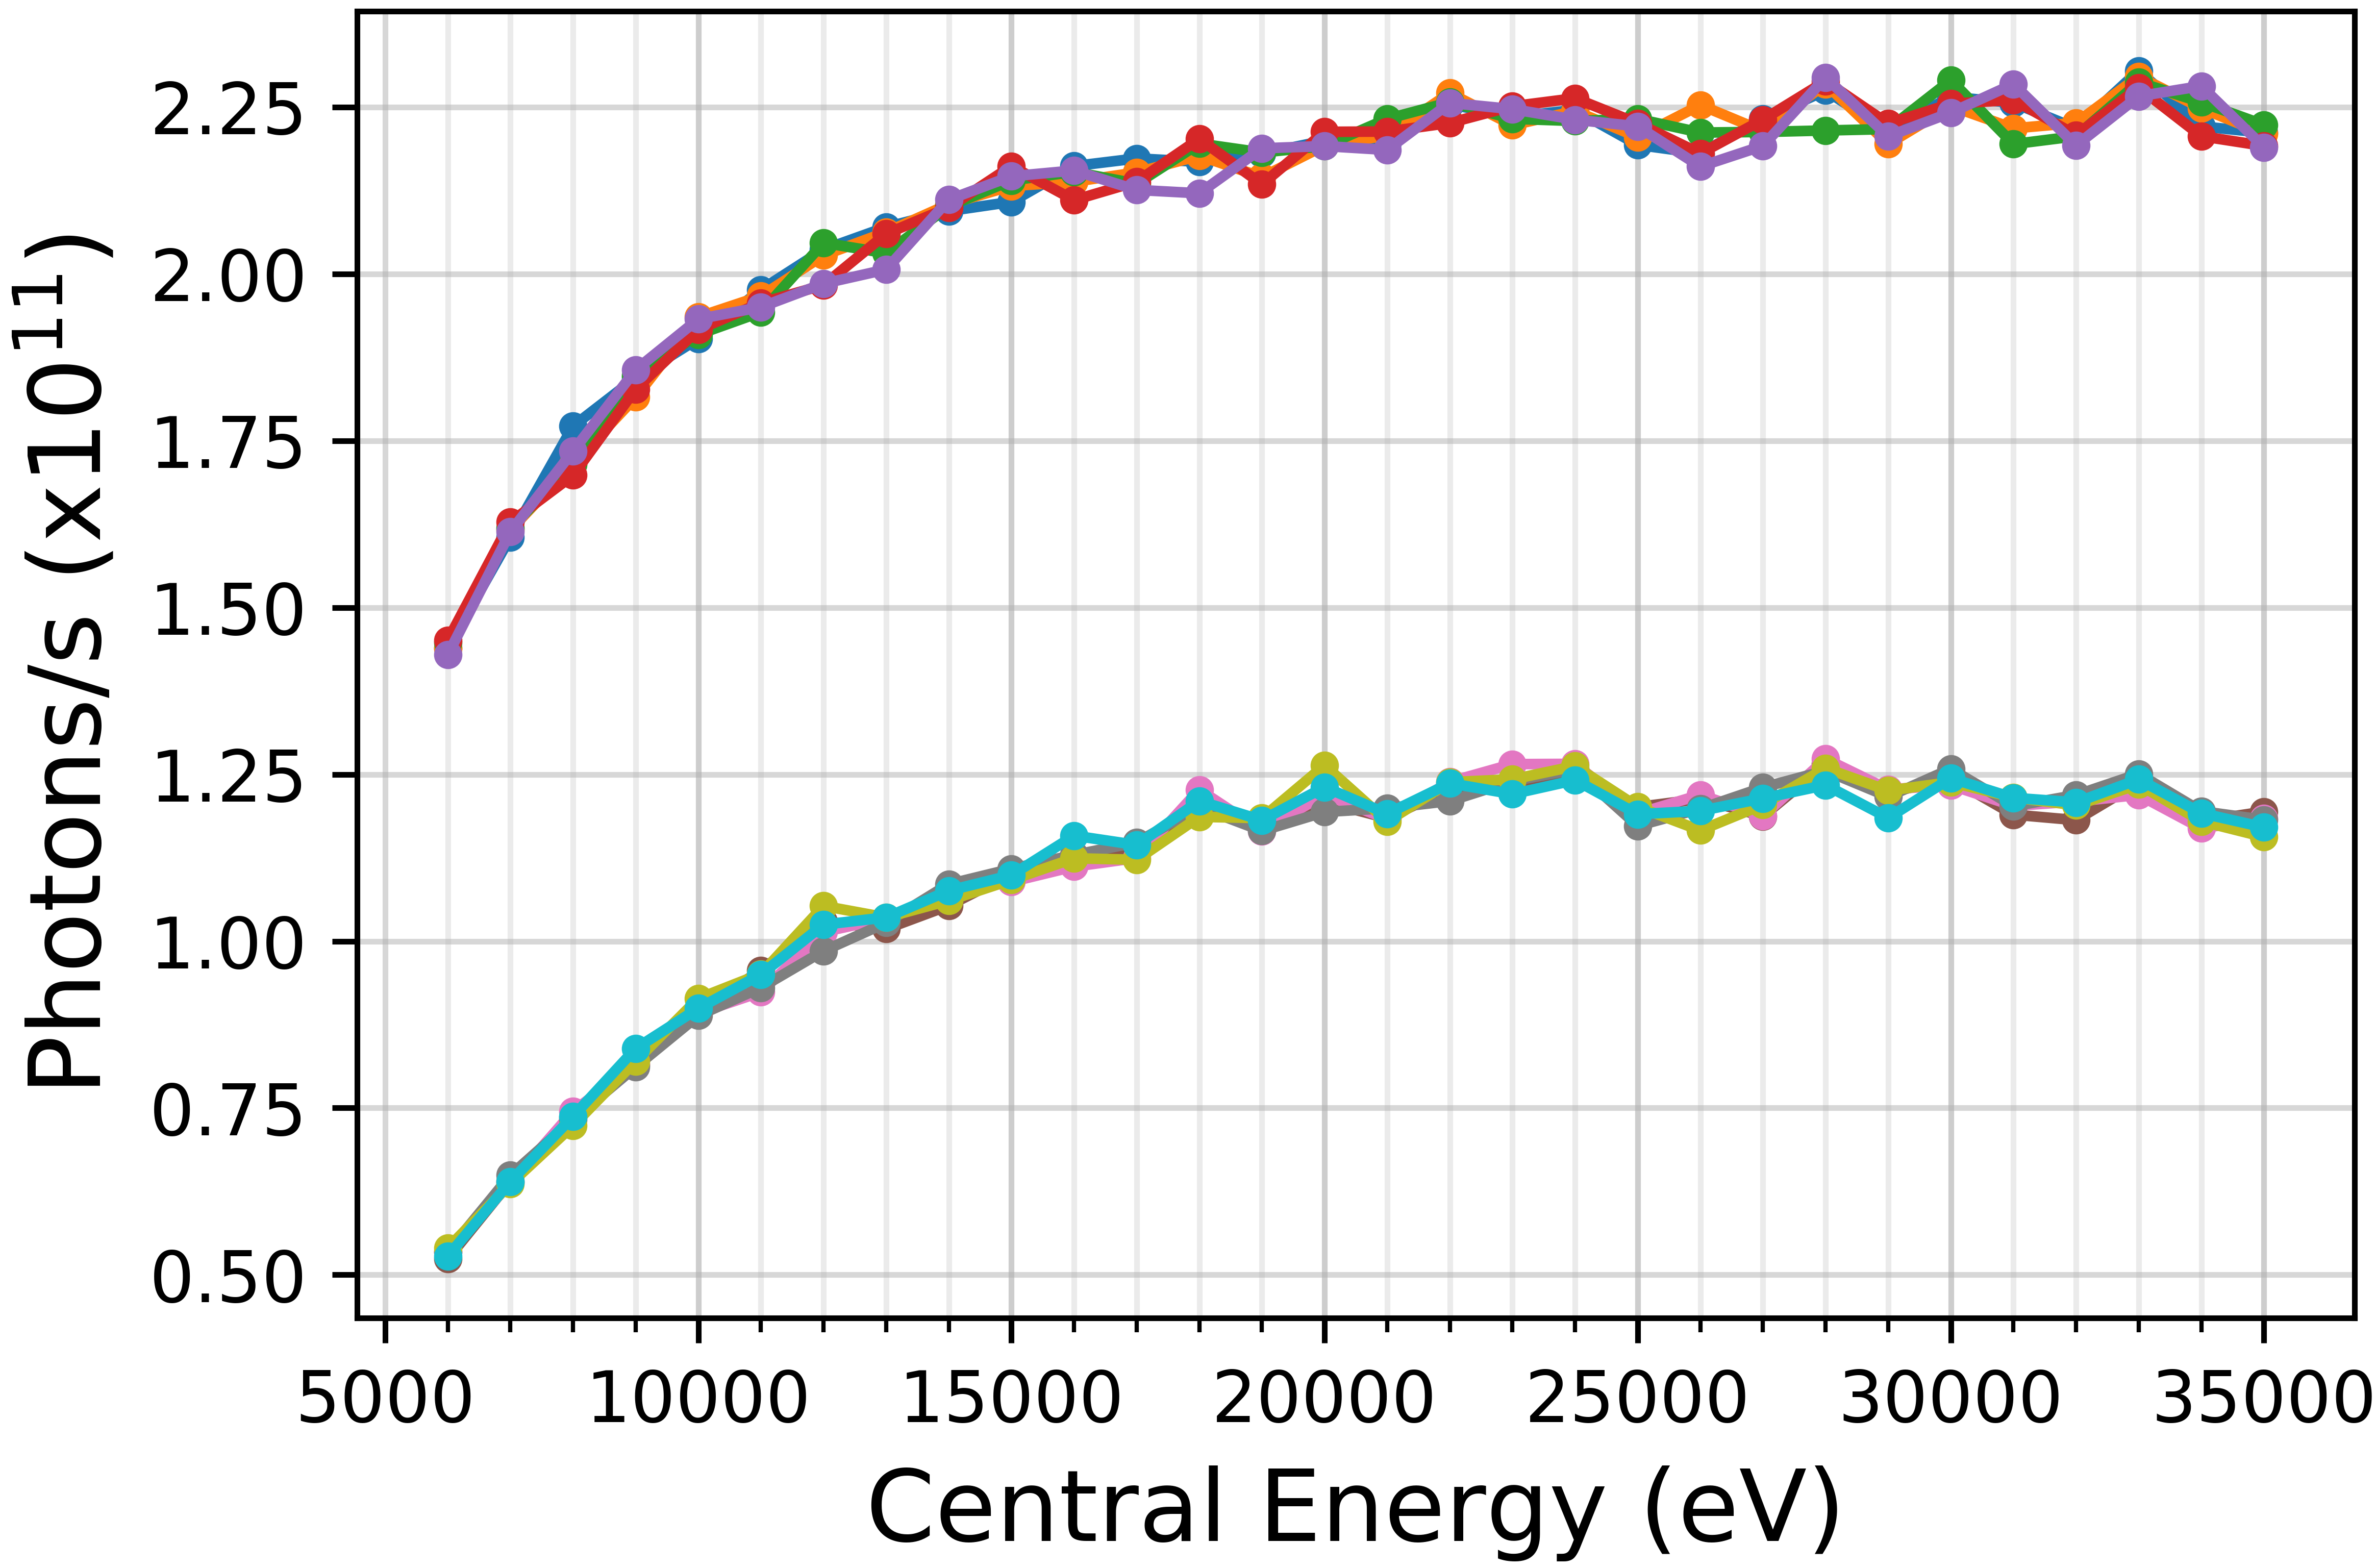
\includegraphics{images/333strainsize.png}
\label{fig:333strainsourcesize}
\end{figure}

\begin{figure}
\caption{in what units?}
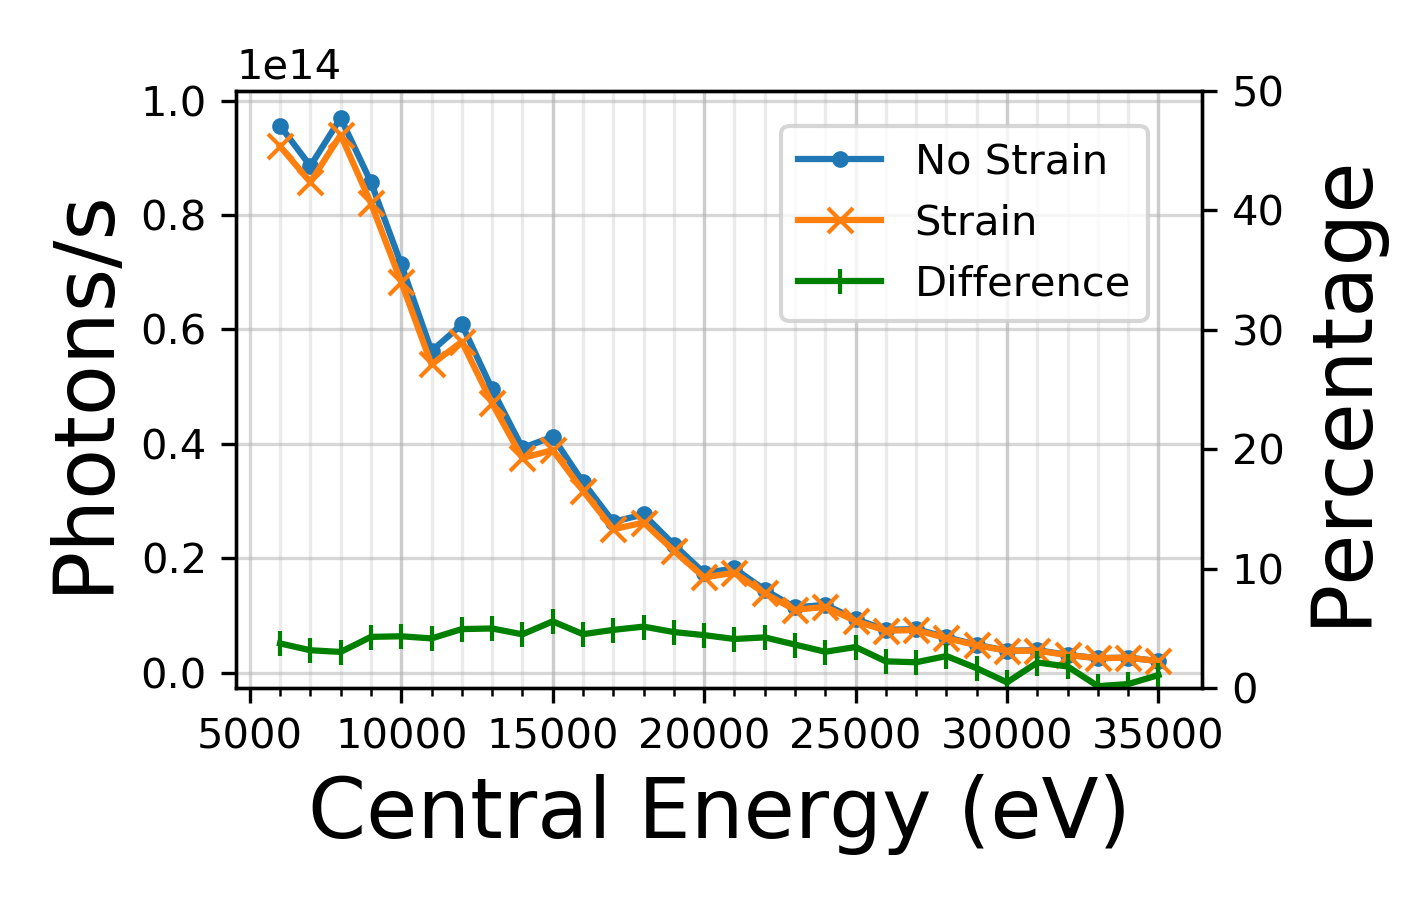
\includegraphics{images/ivu111flux.png}
\label{fig:ivu111flux}
\end{figure}

\begin{figure}
\caption{in what units?}
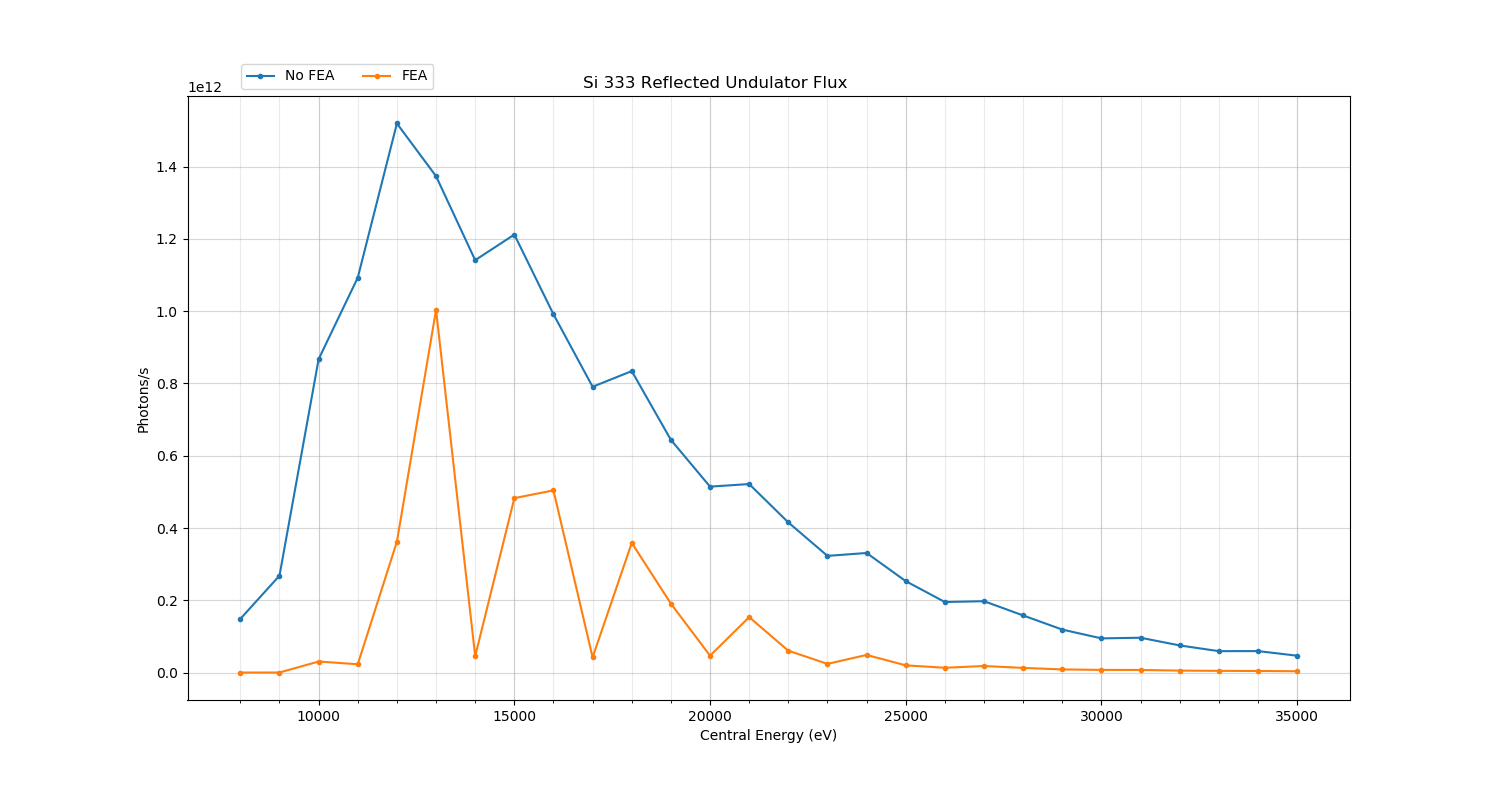
\includegraphics{images/ivu333flux.png}
\label{fig:ivu333flux}
\end{figure}

\begin{figure}
\caption{HI}
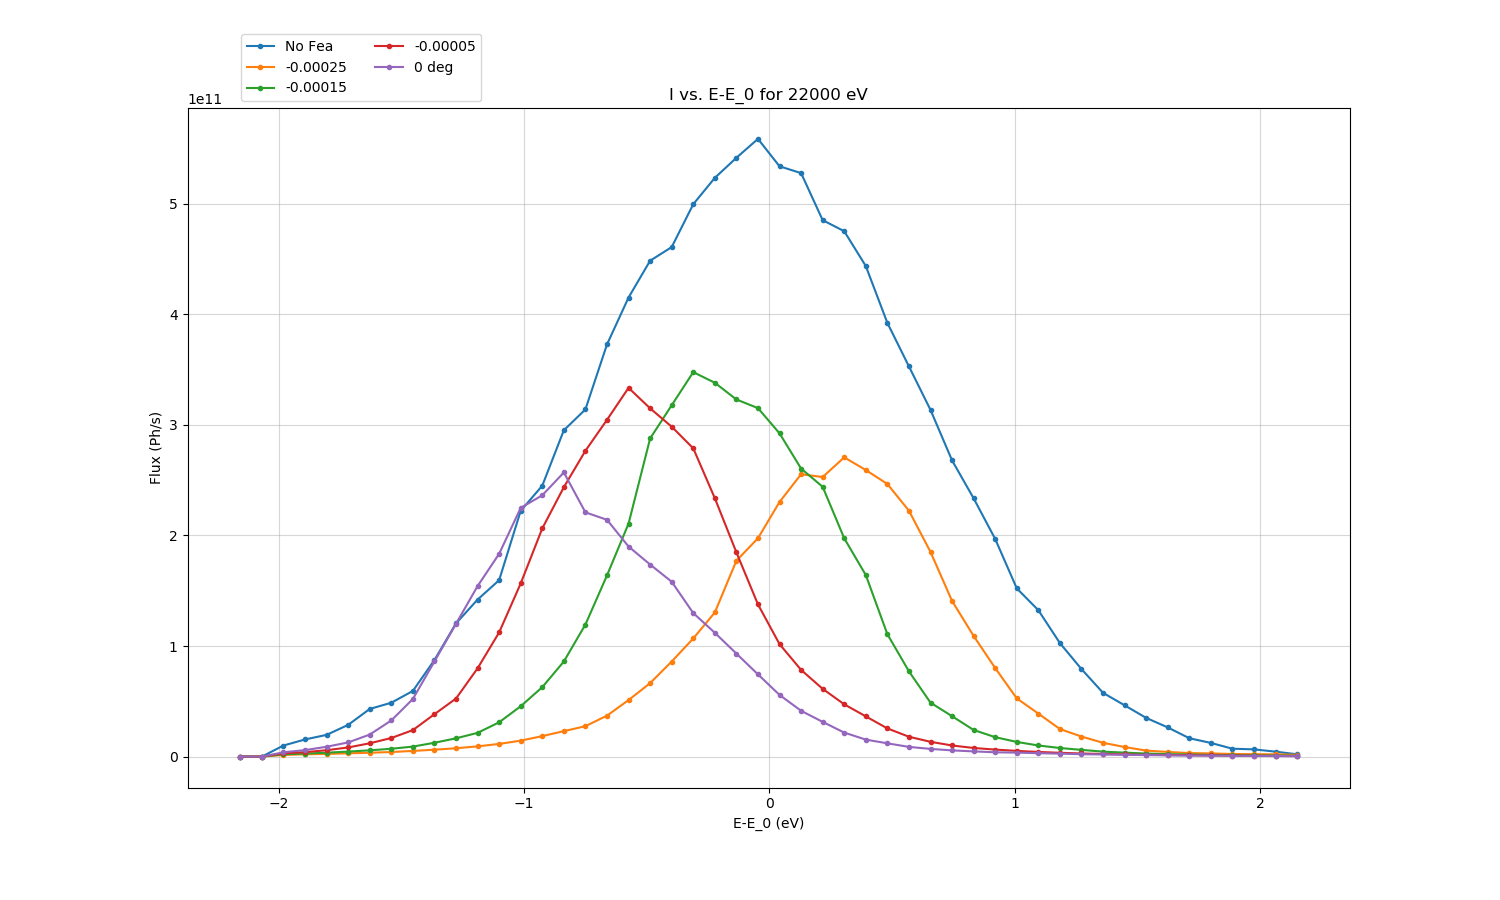
\includegraphics{images/22kevangle.png}
\label{fig:22kevangle}
\end{figure}

\begin{figure}
\caption{HI}
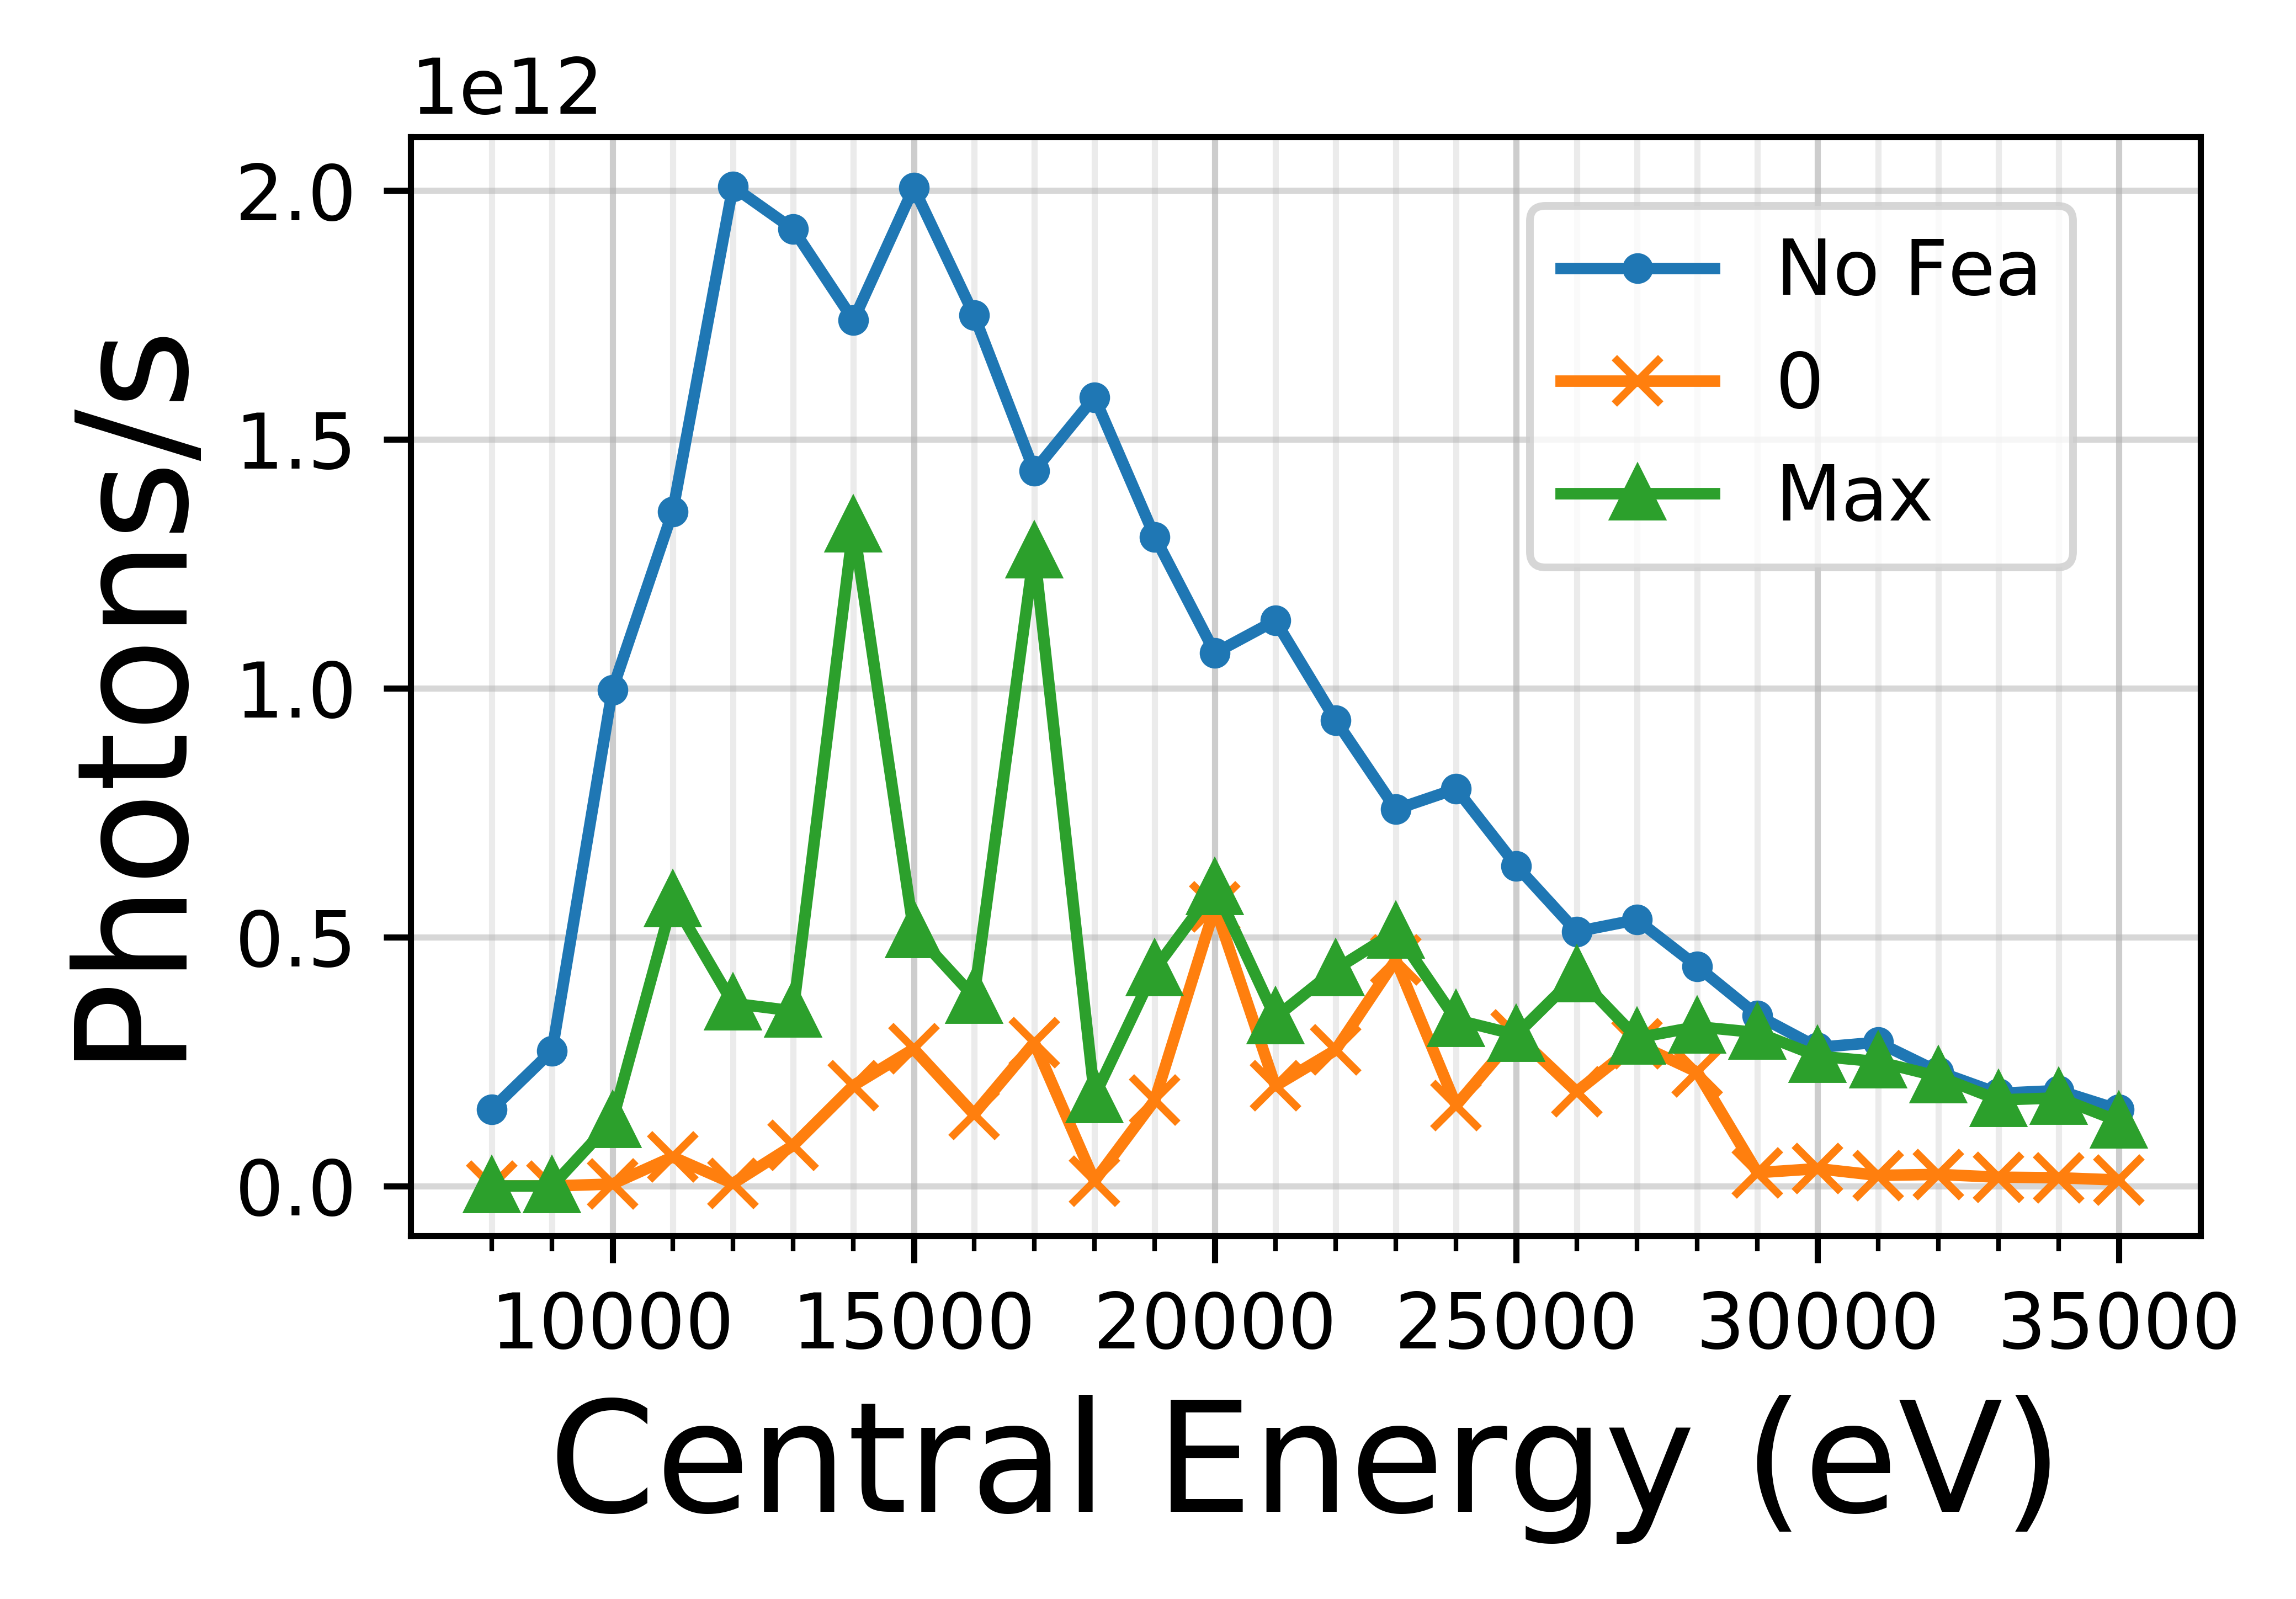
\includegraphics{images/maxangleflux.png}
\label{fig:maxangleflux}
\end{figure}

\begin{table}

\caption{Silicon FEA Parameters}
\begin{tabular}{@{}llll@{}}
Parameter   & Value                   & Units                     & Description                        \\
\hline
$h$           & 0.3                     & W/cm$^2$ $\cdot$K          & Heat transfer coefficient          \\
$T_{cool}$  & 77                      & K                         & Side cooling temperature           \\
$C_{11}$    & $1.6772\times 10^{11}$  & Pa                        & Stiffness tensor 11 component      \\
$C_{12}$    & $6.4980\times 10^{10}$  & Pa                        & Stiffness tensor 12 component      \\
$C_{44}$    & $8.0360\times 10^{10}$  & Pa                        & Stiffness tensor 44 component      \\
$C_p$       & 0.2                     & J/g$\cdot$K               & Heat capacity at constant pressure \\
$\rho$      &  2329                   & kg/m$^3$                  & Density                            \\
\end{tabular}
\label{siliconFEA}
\end{table}


\begin{table}

\caption{Copper FEA Parameters}
\begin{tabular}{@{}llll@{}}
Parameter    & Value                  & Units                      & Description                        \\
\hline
$C_p$        & 385                    & J/kg$\cdot$K               & Heat capacity at constant pressure \\
$\kappa$     & 400                    & W/m$\cdot$K                & Thermal conductivity               \\ 
$\rho$       & 8960                   & kg/m$^3$                   & Density                            \\
\end{tabular}
\label{copperFEA}
\end{table}


\begin{table}
\caption{Indium FEA Parameters}
\begin{tabular}{@{}llll@{}}
Parameter    & Value                  & Units                      & Description                        \\
\hline
$C_p$        & 233                    & J/kg$\cdot$K               & Heat capacity at constant pressure \\
$\kappa$     & 81.6                   & W/m$\cdot$K                & Thermal conductivity               \\
$\rho$       & 7290                   & kg/m$^3$                   & Density                            \\
\end{tabular}
\label{indiumFEA}
\end{table}


\begin{table}
\caption{Liquid Nitrogen FEA Parameters}
\begin{tabular}{@{}llll@{}}
Parameter    & Value                  & Units                       & Description                        \\
\hline
$\mu$        & $157.9\times 10^{-6}$  & Pa$\cdot$s                  & Dynamic viscosity                  \\ 
$\gamma$     & 1.47                   & 1				            & Ratio of specific heats            \\
$C_p$        & 2.04                   & kJ/kg$\cdot$K               & Heat capacity at constant pressure \\
$\kappa$     & 139.6                  & mW/m$\cdot$K                & Thermal conductivity               \\
$\rho$       & 0.807                  & g/ml                        & Density                            \\
\end{tabular}
\label{nitogrenFEA}
\end{table}


\end{document}                    % DO NOT DELETE THIS LINE
%%%%%%%%%%%%%%%%%%%%%%%%%%%%%%%%%%%%%%%%%%%%%%%%%%%%%%%%%%%%%%%%%%%%%%%%%%%%%%
